\renewcommand{\chaptername}{BAB}
%-----------------------------------------------------------------------------%
\chapter{HASIL DAN PEMBAHASAN}
%-----------------------------------------------------------------------------%
\vspace{4.5pt}
\setlength{\parskip}{0.5em}
\section{Perancangan (Design)}\label{sec:bab4_perancangan}
Pada tahan pertama ini peneliti akan melakukan perancangan sebuah infrastruktur
dimana sistem Kubernetes dan ArgoCD akan dijalankan lalu microservice untuk
dilakukan simulasi implementasi pada ArgoCD. Semua rancangan akan menggunakan
visualisasi diagram secara garis besar (high-level) agar mudah dipahami.

\subsection{Perancangan Sistem Arsitektur Infrastruktur Mesin}
Sebelum dilakukan penelitian lebih lanjut pada implementasi ArgoCD pada
Kubernetes Cluster perlu dirancang terlebih dahulu arsitektur infrastruktur
mesin yang akan menjadi tempat instlasi Kubernetes Cluster. Peneliti
menggunakan Proxmox VE (Virtual Environment) yang didalam nya terdapat Virtual
Machine berupa Talos OS Linux yang siap dilakukan instalasi Kubernetes Cluster.
\begin{figure}[H]
  \centering
  \fcolorbox{black}{white}{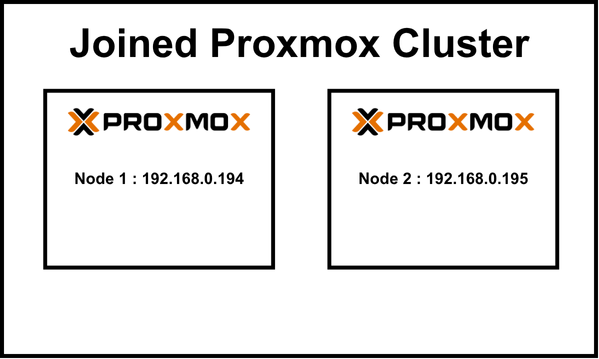
\includegraphics[width=0.9\textwidth]{figures/proxmox-cluster-design-1.png}}
  \caption{Arsitektur Infrastruktur High Level}
  \label{fig:arsitektur_infrastruktur_mesin}
\end{figure}
Pada \textbf{Gambar \ref{fig:arsitektur_infrastruktur_mesin}} menunjukan
arsitektur infrastruktur mesin secara high level dimana terdapat 2 cluster
proxmox yang di \textit{joined} agar bisa saling terhubung satu sama lain.
Akses terhadap proxmox tersebut dapat dilakukan menggunakan port 8006 dengan
menggunakan browser atau dengan kata lain bisa diakses dari
https://192.168.0.194:8006/ atau https://192.168.0.195:8006/
\begin{figure}[H]
  \centering
  \fcolorbox{black}{white}{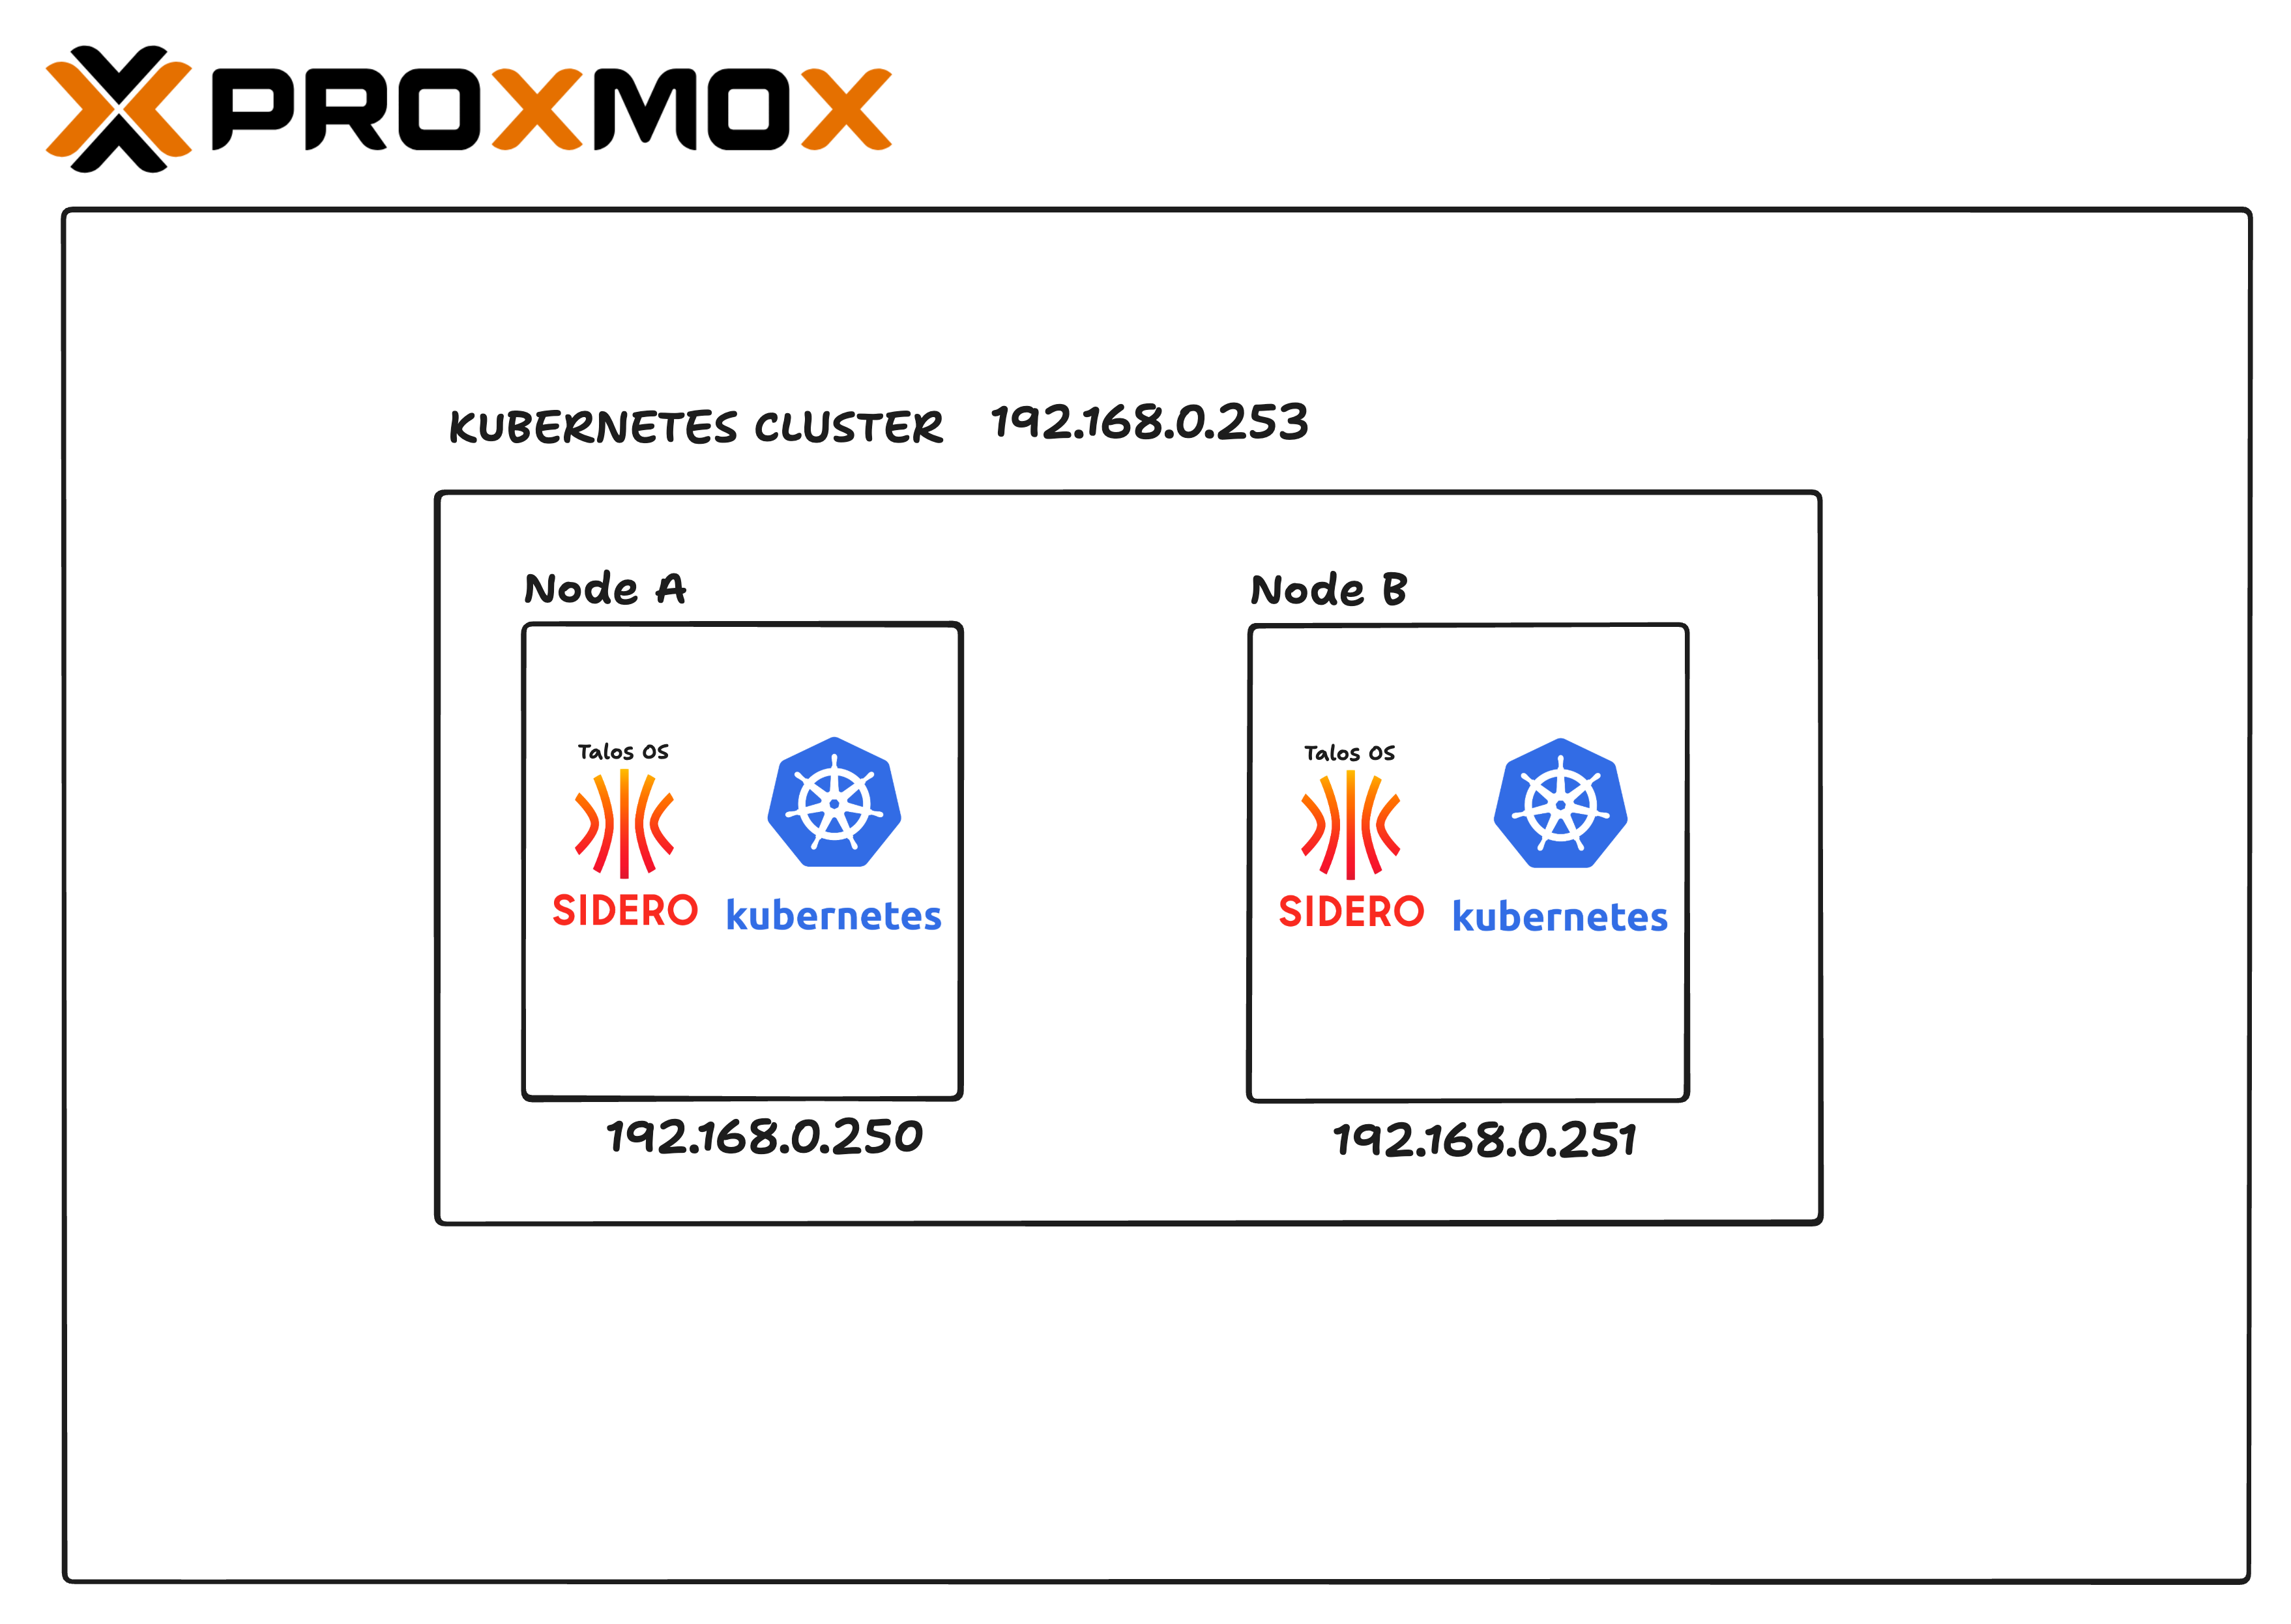
\includegraphics[width=0.9\textwidth]{figures/proxmox-cluster.png}}
  \caption{Arsitektur Virtual Machine Talos OS pada Proxmox Cluster}
  \label{fig:arsitektur_virtual_machine_talos_os}
\end{figure}

Setelah dilakukan \textit{provisioning} pada proxmox tersebut akan dilakukan
instalasi Talos OS pada node tersebut menggunakan dengan memanfaatkan
\textit{virtual machine} yang ada pada proxmox. Pada \textbf{Gambar
  \ref{fig:arsitektur_virtual_machine_talos_os}} merupakan arsitektur pada
kubernetes cluster itu sendiri dimana sistem virtual machine yang didalamnya
terdapat komponen Talos OS dan komponen kubernetes. Kubernetes Cluster dapat
diakses menggunakan address 192.168.0.253:6443 menggunakan kubectl didalam
address tersebut terdapat 2 node Talos OS yang masing-masing memiliki komponen
kubernetes node.

\subsection{Perancangan Arsitektur ArgoCD pada Kubernetes Cluster}
Pada bagian sebelumnya peneliti sudah memaparkan arsitektur infrastruktur mesin
dimana Kubernetes cluster akan berjalan. Pada tahap ini peneliti akan
memaparkan arsitektur pada kubernetes cluster nya itu sendiri dimana ArgoCD
akan berjalan.
\begin{figure}[H]
  \centering
  \fcolorbox{black}{white}{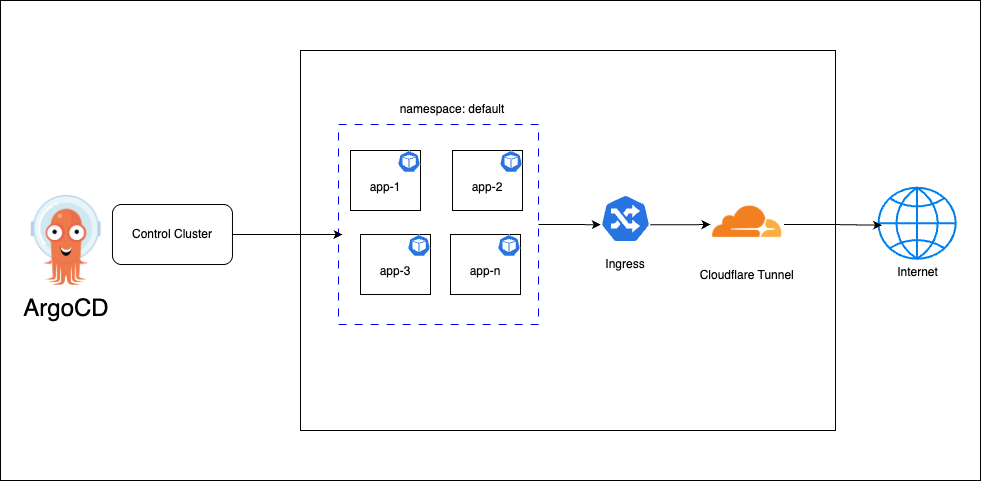
\includegraphics[width=0.9\textwidth]{figures/kubernetes-cluster-1-new.png}}
  \caption{Arsitektur Kubernetes High Level}
  \label{fig:arsitektur_kubernetes_inside_proxmox}
\end{figure}

Pada \textbf{Gambar \ref{fig:arsitektur_kubernetes_inside_proxmox}}
mengambarkan arsitektur kubernetes nya secara high level dimana terdapat
komponen ArgoCD dan Cloudflare Tunnel yang bertujuan agar server microservice
bisa diakses pada world wide web (internet). Secara garis besar sebuah service
digambarkan sebagai app yang terdeploy pada sebuah namespace yang terdapat pada
kubernetes cluster. Lalu \textit{ingress} akan digunakan untuk mengakses
service tersebut dari luar cluster dengan menggunakan domain yang sudah
terdaftar pada cloudflare.

\subsection{Perancangan Arsitektur Microservice pada Kubernetes Cluster}
Pada bagian ini peneliti akan memaparkan contoh design arsitektur microservice
yang akan dijadikan acuan untuk dilakukan implementasi pada kubernetes cluster.
Nantinya service service ini akan berdiri sendiri dan mempunya deployment
sendiri pada kubernetes cluster. Deployment service tersebut akan dideploy
menggunakan ArgoCD agar bisa terdeploy kedalam kubernetes cluster.
\begin{figure}[H]
  \centering
  \fcolorbox{black}{white}{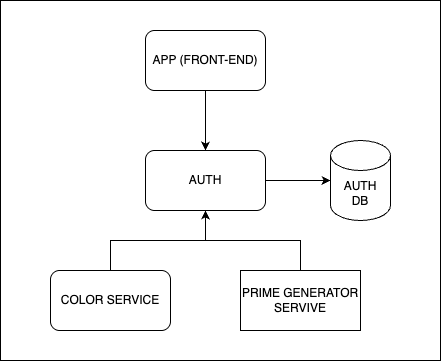
\includegraphics[width=0.9\textwidth]{figures/microservice-arsitektur.drawio.png}}
  \caption{Arsitektur Microservice High Level}
  \label{fig:arsitektur_microservice_high_level}
\end{figure}

Pada \textbf{Gambar \ref{fig:arsitektur_microservice_high_level}} menggambarkan
arsitektur microservice yang akan dideploy pada kubernetes cluster menggunakan
Argo CD. Microservice tersebut terdiri dari beberapa service yaitu service
frontend yang akan berfungsi sebagai interface untuk user dan service backend
yang akan diakses. Terdapat juga service auth yang akan berfungsi sebagai
autentikasi dan otorisasi user sebelum bisa mengakses service backend yaitu
color service dan prime generator service. Auth service sendiri bersifat
stateless komponen auth db pada arsitektur digambarkan untuk menyimpan data
user yang akan diakses oleh service auth. Color service dan prime generator
service sendiri juga bersifat stateless untuk mempermudah implementasi
microservice tersebut.

\section{Pengkodean (Coding) / Implementasi}\label{sec:bab4_implementasi}
Tahap ini peneliti akan menjabarkan secara rinci pengkodean/implementasi
rancangan sistem yang sudah dirancang sebelumnya pada bagian
\textbf{\ref{sec:bab4_perancangan} Perancangan (Design)}. Tahap implementasi
akan dijelaskan secara berurutan sesuai dengan urutan yang dijabarkan
sebelumnya pada bagian \textbf{\ref{sec:bab4_perancangan} Perancangan
  (Design)}.

\subsection{Implementasi Sistem Infrastruktur Mesin}\label{sec:bab4_instalasi_infrastruktur_mesin}
Untuk implementasi infrastruktur mesin. Peneliti akan melakukan instalasi
proxmox pada 2 mesin dengan arsitektur CPU X86. \textbf{Tabel
  \ref{tab:node-kubernetes}} merupakan spesifikasi node yang akan digunakan pada
penelitian ini.

\begin{table}[H]
  \centering
  \begin{tabular}{|l|l|l|c|c|c|}
    \hline
    \textbf{Node} & \textbf{Host} & \textbf{OS}    & \textbf{CPU (Core)} & \textbf{RAM} & \textbf{Kubernetes Version} \\
    \hline
    master-1      & 192.168.0.194 & Talos OS 1.9.5 & 4                   & 12 GB        & v1.28.0                     \\
    \hline
    worker-1      & 192.168.0.195 & Talos OS 1.9.5 & 4                   & 12 GB        & v1.28.0                     \\
    \hline
  \end{tabular}
  \caption{Spesifikasi Node Kubernetes}
  \label{tab:node-kubernetes}
\end{table}
\begin{figure}[H]
  \centering
  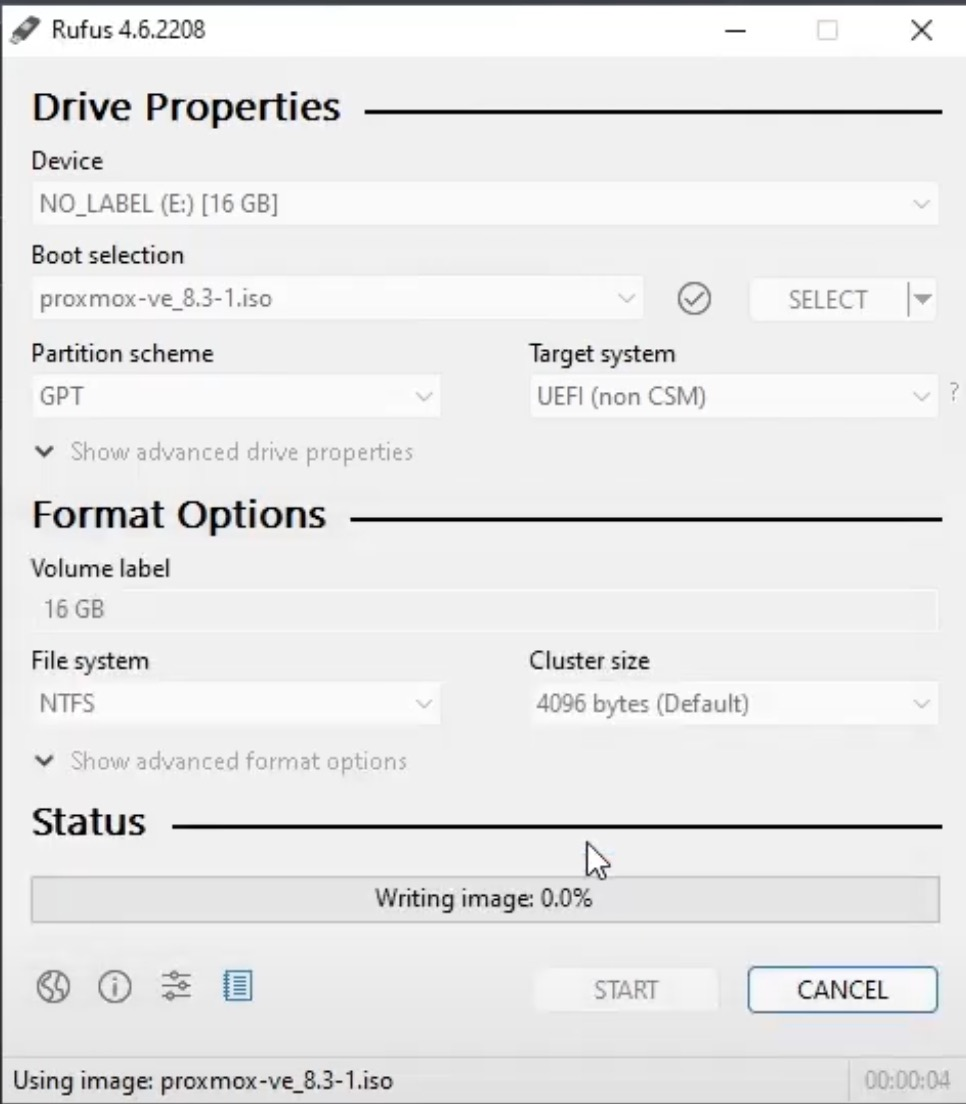
\includegraphics[width=0.8\textwidth]{figures/proxmox-install-rufus-1.jpg}
  \caption{Pembuatan Bootable Proxmox Menggunakan Rufus}
  \label{fig:proxmox_rufus}
\end{figure}
Pertama peneliti akan download ISO file atau installer proxmox yang terdapat di
link ini \verb|https://enterprise.proxmox.com/iso/proxmox-ve_8.4-1.iso|. Setelah
itu peneliti memerlukan sebuah Flashdisk atau media untuk bootable ISO
tersebut disini peneliti menggunakan tools yang bernama Rufus seperti pada \textbf{Gambar \ref{fig:proxmox_rufus}}. Setelah itu kita perlu mengganti bootable menu yang mengarah pada flashdisk
atau media yang kita gunakan untuk instalasi proxmox ketika booting BIOS pada
mesin yang digunakan. Setelah itu mesin akan restart dan akan masuk pada tampilan
seperti pada \textbf{Gambar \ref{fig:proxmox_install_ui}}.

\begin{figure}[H]
  \centering
  \fcolorbox{black}{white}{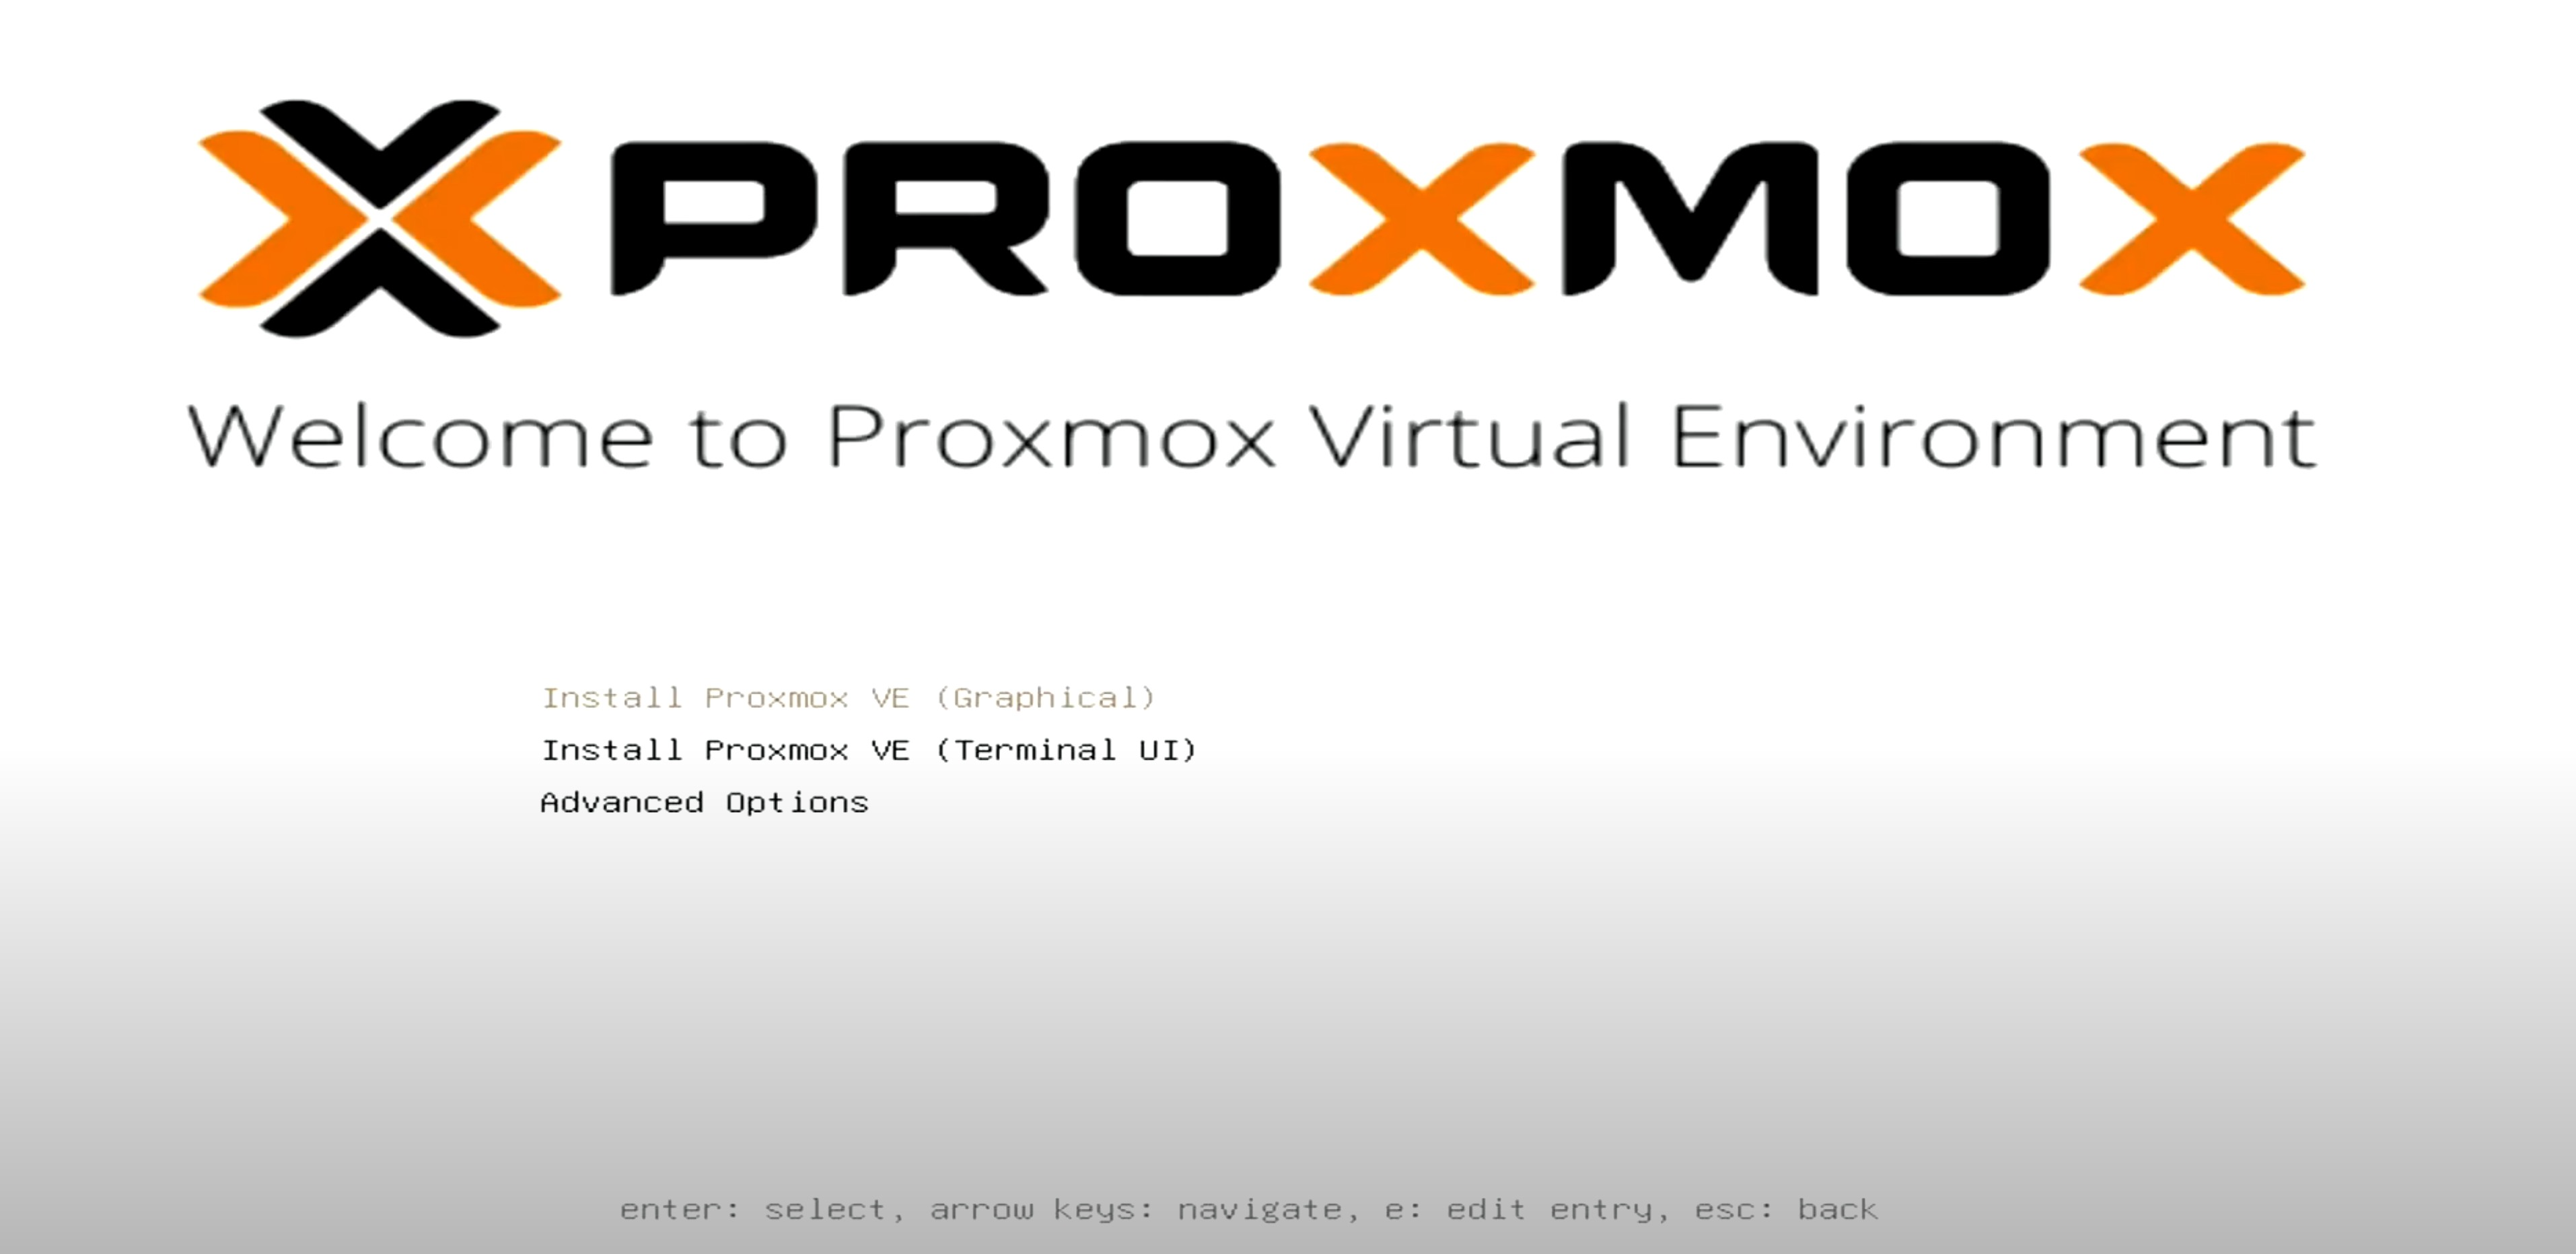
\includegraphics[width=0.8\textwidth]{figures/proxmox-install-ui-2.jpg}}
  \caption{Tampilan Awal Instalasi Proxmox VE}
  \label{fig:proxmox_install_ui}
\end{figure}

Selanjutnya kita tinggal mengikuti apa yang diarahkan secara default oleh user
interface yang ditampilkan hingga mesin akan restart dan berada pada tampilan
seperti pada \textbf{Gambar \ref{fig:proxmox_terminal}}. Pada tampilan layar
tersebut terdapat alamat server yang bisa kita gunakan untuk akses user
interface melalui browser.
\begin{figure}[H]
  \centering
  \fcolorbox{black}{white}{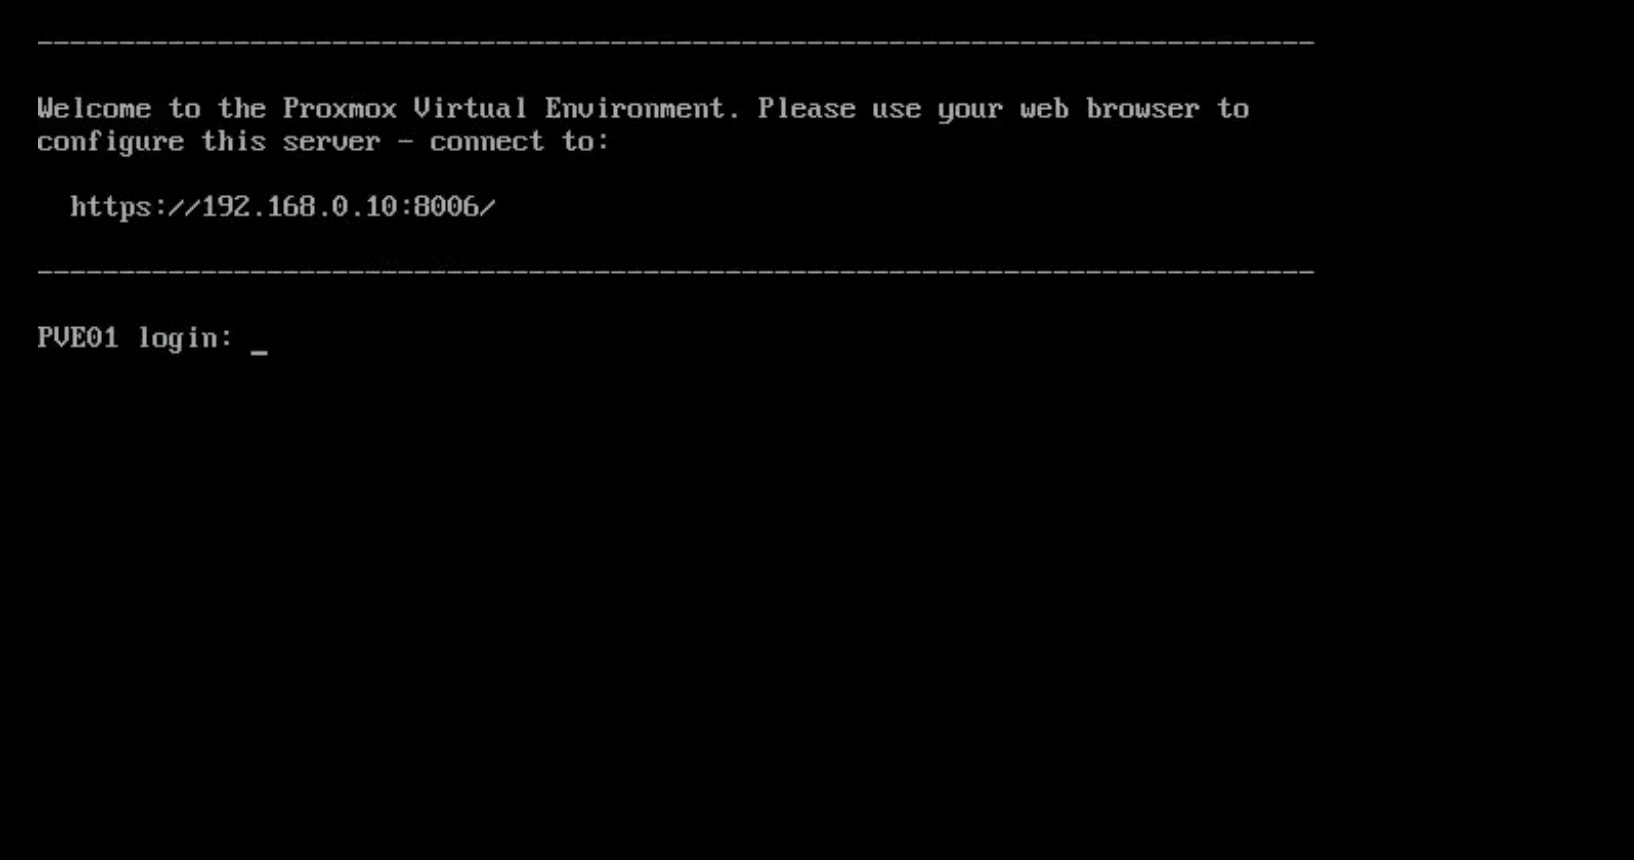
\includegraphics[width=0.8\textwidth]{figures/proxmox-install-terminal-3.jpg}}
  \caption{Tampilan Terminal Setelah Instalasi Proxmox Selesai}
  \label{fig:proxmox_terminal}
\end{figure}

Akses UI pada komputer yang ada pada network yang sama dengan Proxmox melalui
web alamat server yang terlihat pada gambar \textbf{Gambar
  \ref{fig:proxmox_terminal}} maka akan muncul tampilan seperti pada
\textbf{Gambar \ref{fig:proxmox_webui}}. Peneliti akan mengulang implementasi
ini untuk mesin kedua dengan step yang sama seperti pada mesin pertama.
\begin{figure}[H]
  \centering
  \fcolorbox{black}{white}{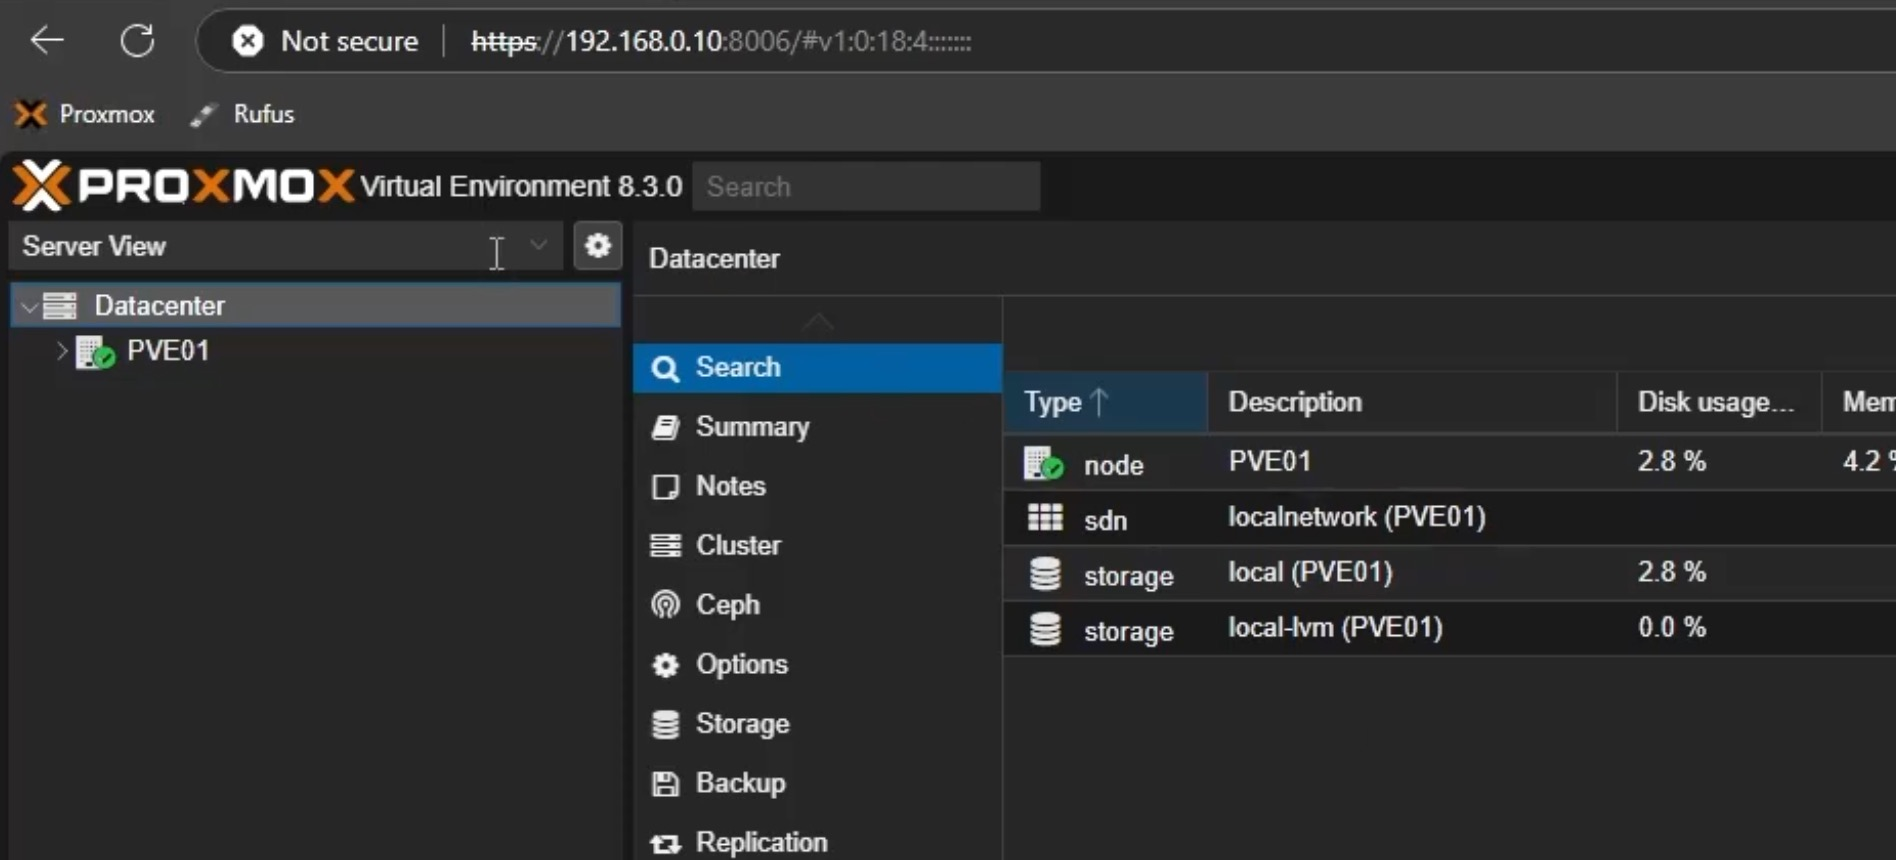
\includegraphics[width=0.9\textwidth]{figures/proxmox-install-web-ui-4.jpg}}
  \caption{Tampilan Web Interface Proxmox VE}
  \label{fig:proxmox_webui}
\end{figure}

Pada tahap selanjutnya akan dilakukan instalasi Talos OS yang akan di-install
menggunakan VM yang ada pada Proxmox VE. Pertama yang dilakukan adalah
mengunduh ISO file Talos OS di sini.

\url{https://github.com/siderolabs/talos/releases/download/v1.9.5/metal-amd64.iso}

\begin{figure}[H]
  \centering
  \fcolorbox{black}{white}{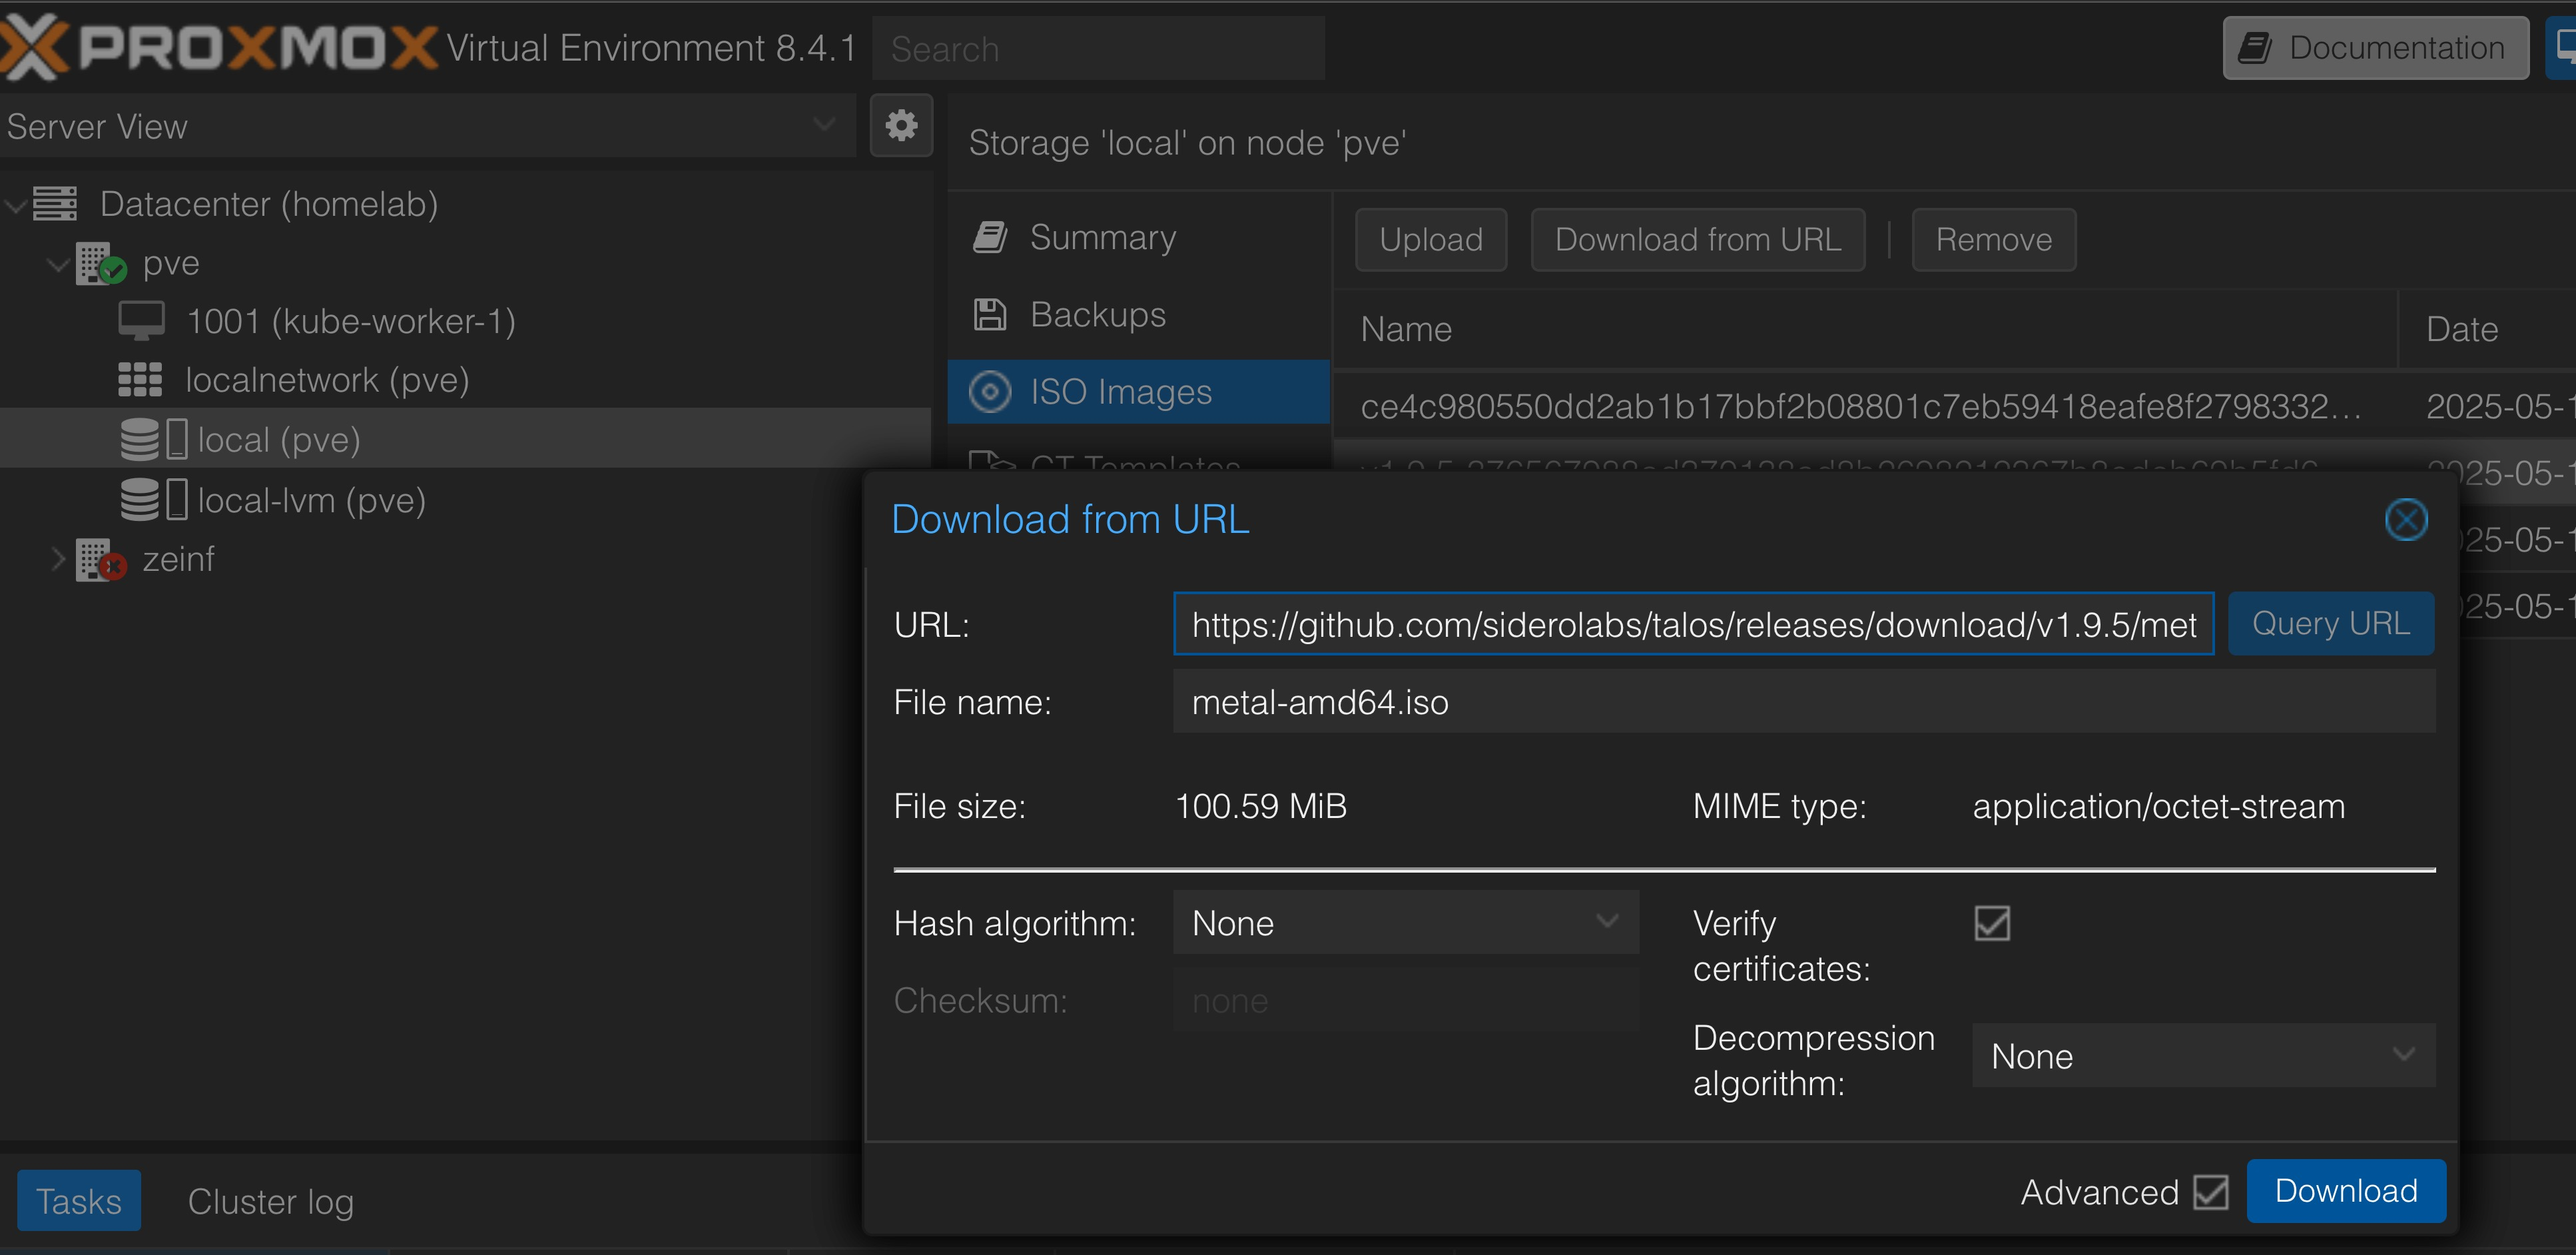
\includegraphics[width=0.8\textwidth]{figures/talos-install-1.jpg}}
  \caption{Proses Download ISO Talos OS}
  \label{fig:talos_download}
\end{figure}

Url tersebut lalu didownload melalui proxmox agar tersimpan didalam proxmox
seperti pada \textbf{Gambar \ref{fig:talos_download}}. Lalu tahap selanjutnya
adalah melakukan instalasi VM Talos OS pada proxmox. Tahap ini adalah bagian
instalasi VM Talos OS. Peneliti melakukan instalasi pada proxmox VE melalui
interface web. Tahap ini akan dilakukan pada 2 mesin berbeda pada proxmox.
Tahap-tahap instalasi Talos OS tersebut dijabarkan secara berurutan yang
ditunjukkan pada \textbf{Gambar \ref{fig:talos_install_1} -
  \ref{fig:talos_install_9}}

\begin{figure}[!htbp]
  1. Klik Create VM lalu isikan VM ID dan Name untuk VM Talos OS
  \centering
  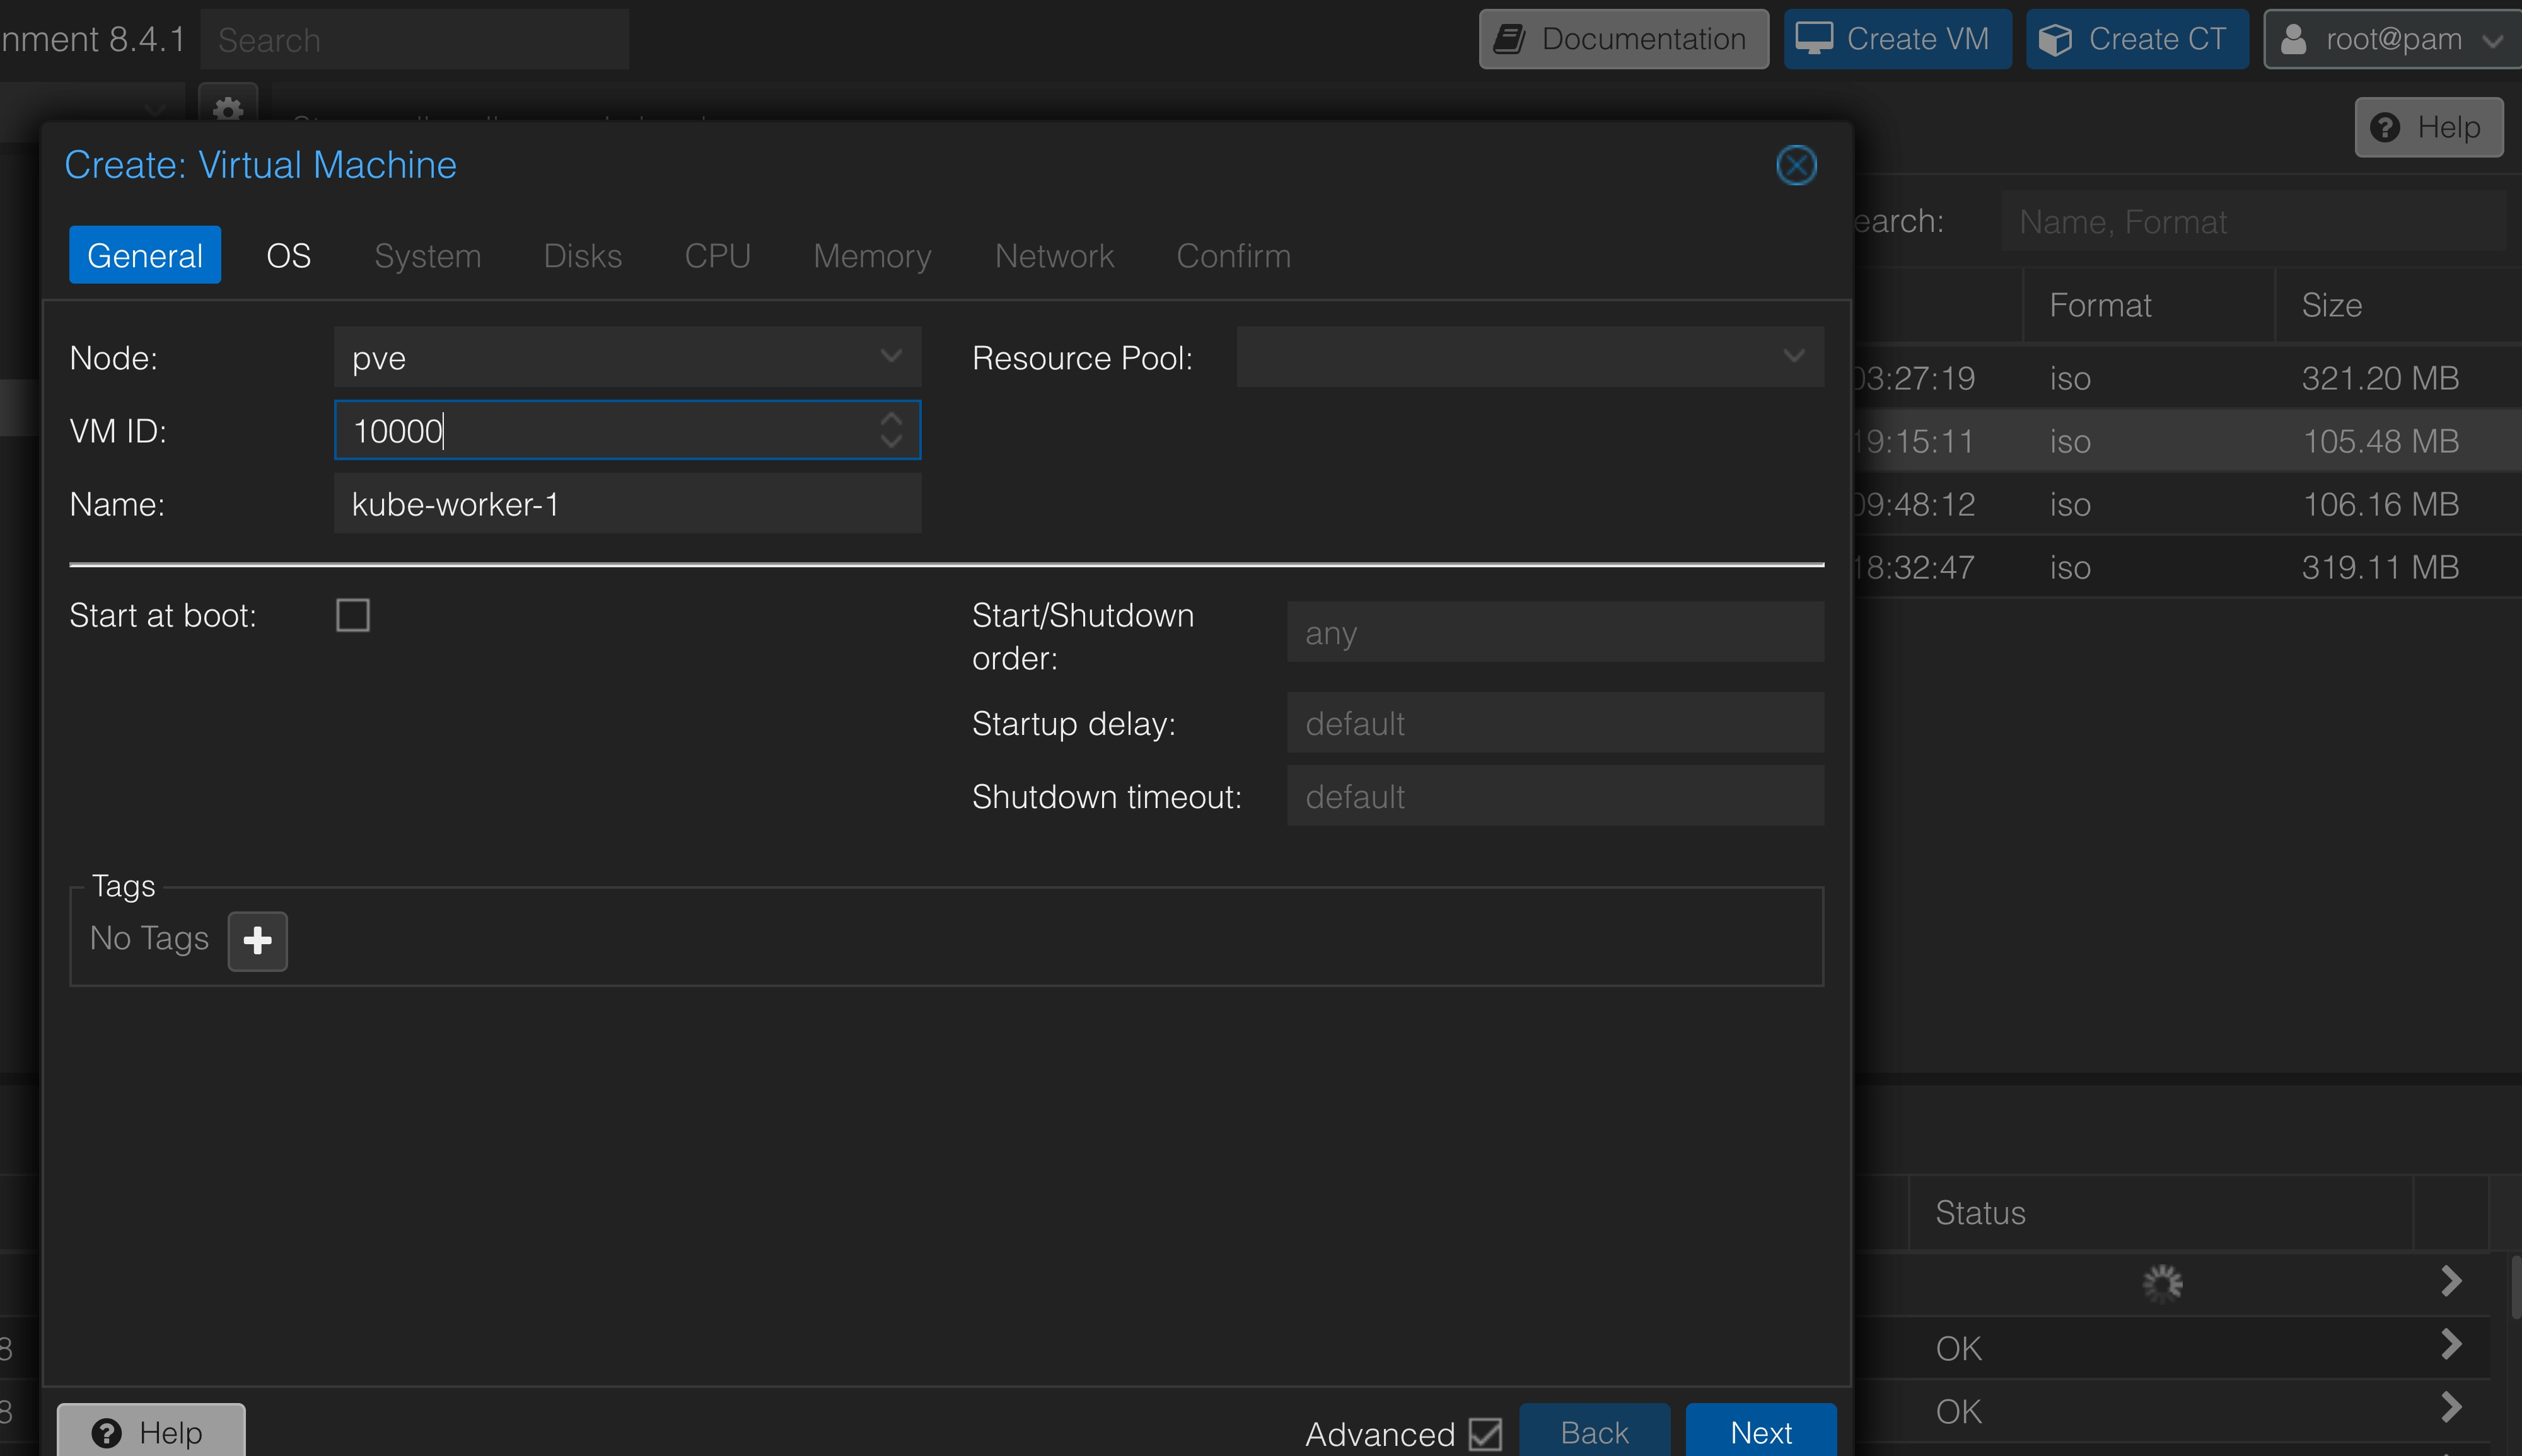
\includegraphics[width=1\textwidth]{figures/talos-install-2.jpg}
  \caption{Instalasi Talos OS 1}
  \label{fig:talos_install_1}
\end{figure}
\begin{figure}[!htbp]
  2. Pada bagian OS. Pilih ISO Talos OS yang baru saja diunduh sebelum nya
  \centering
  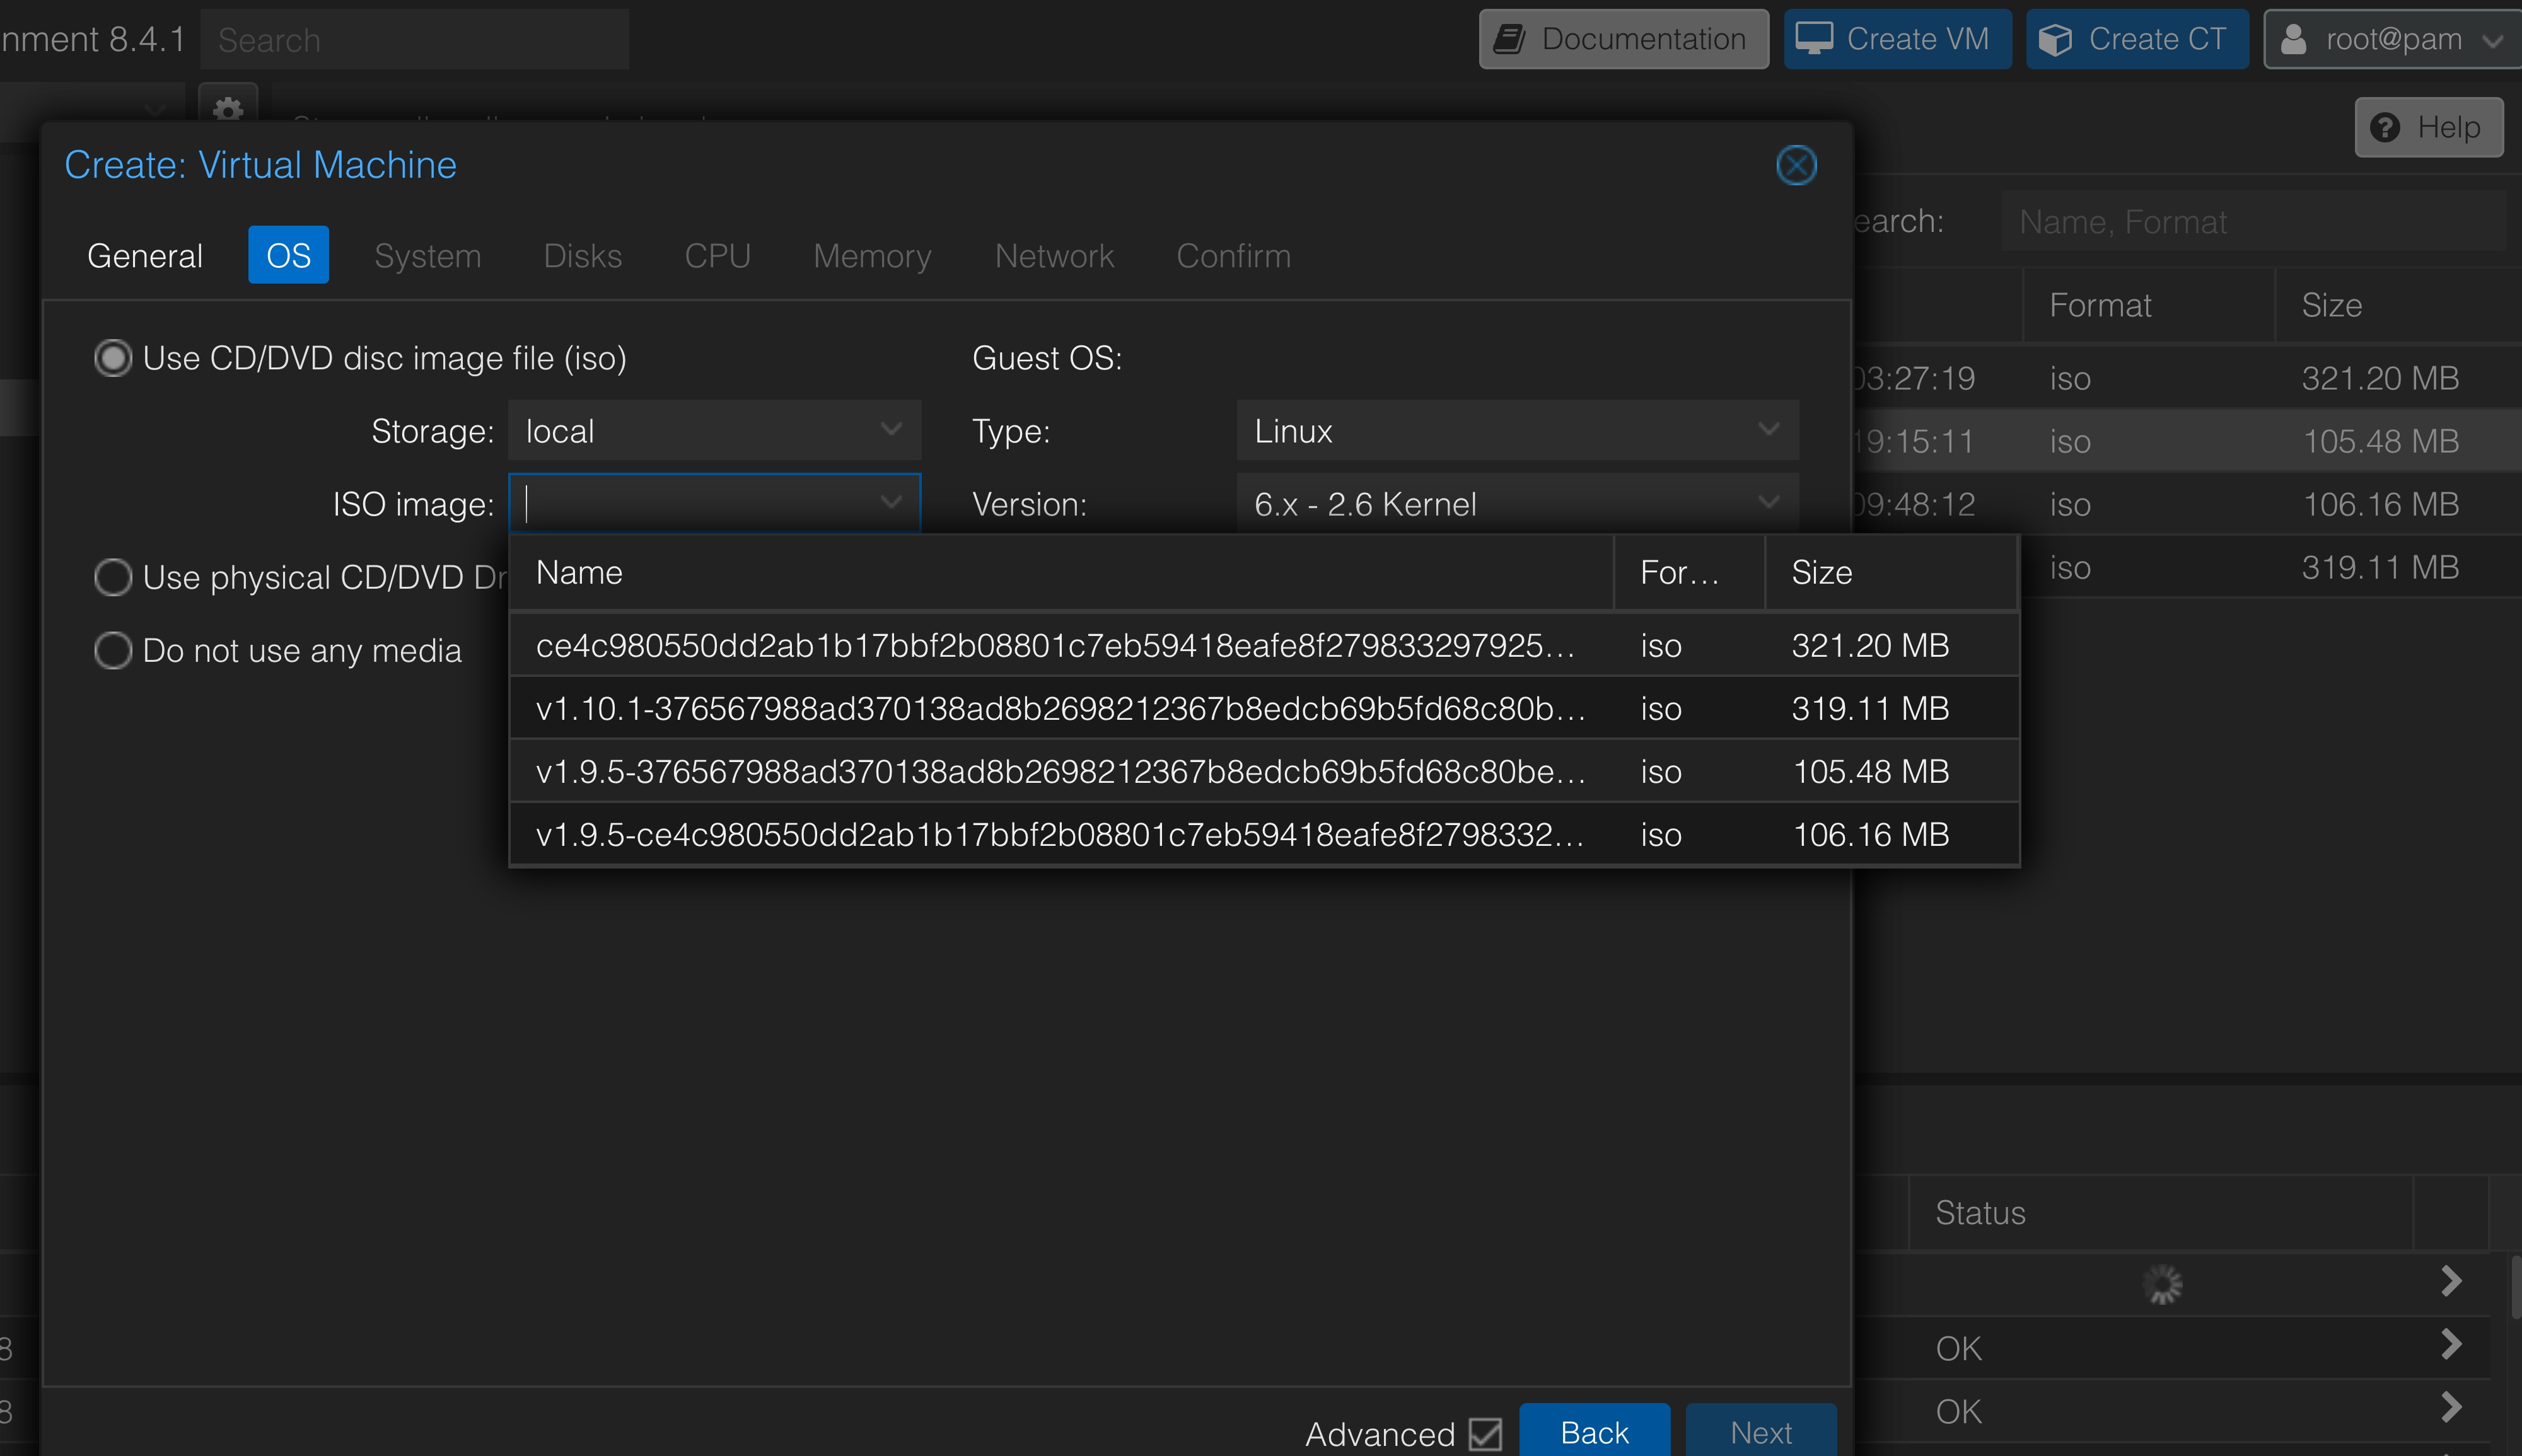
\includegraphics[width=1\textwidth]{figures/talos-install-3.jpg}
  \caption{Instalasi Talos OS 2}
  \label{fig:talos_install_2}
\end{figure}
\begin{figure}[!htbp]
  3. Pada bagian System. cukup next
  \centering
  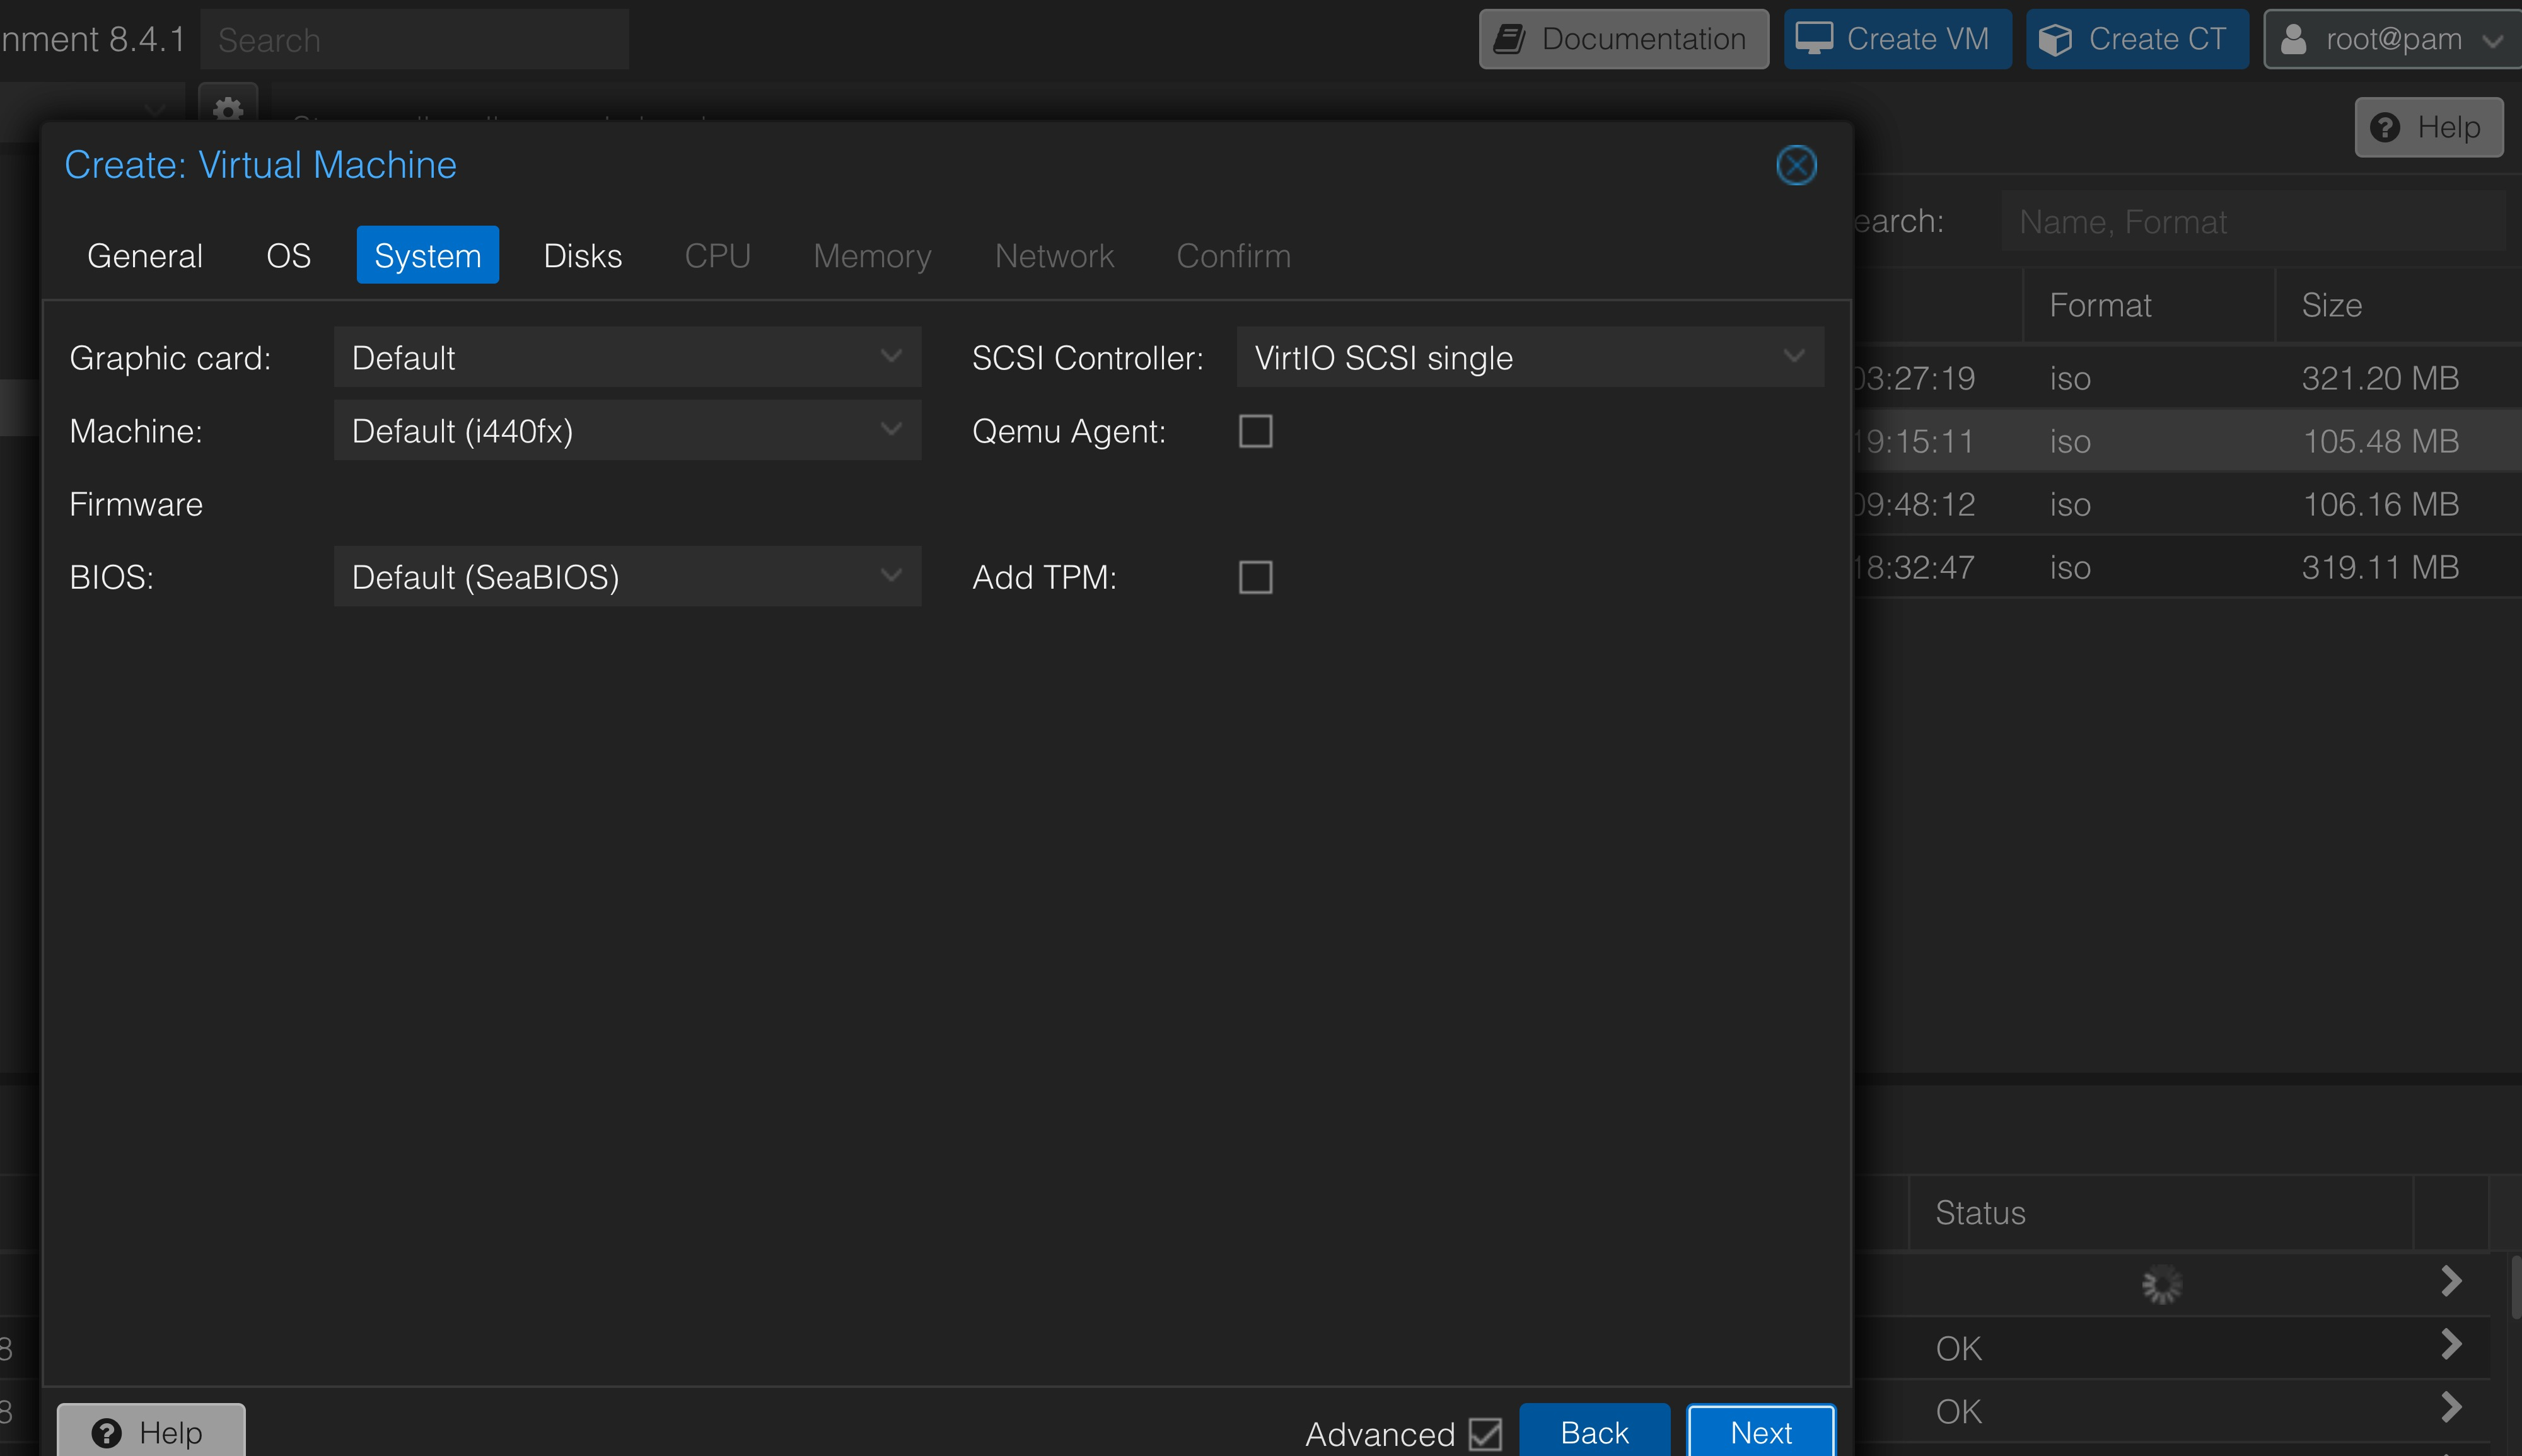
\includegraphics[width=1\textwidth]{figures/talos-install-4.jpg}
  \caption{Instalasi Talos OS 3}
  \label{fig:talos_install_3}
\end{figure}
\begin{figure}[!htbp]
  4. Pada bagian Disk. Cuku merubah bagian Disk size menjadi 100
  \centering
  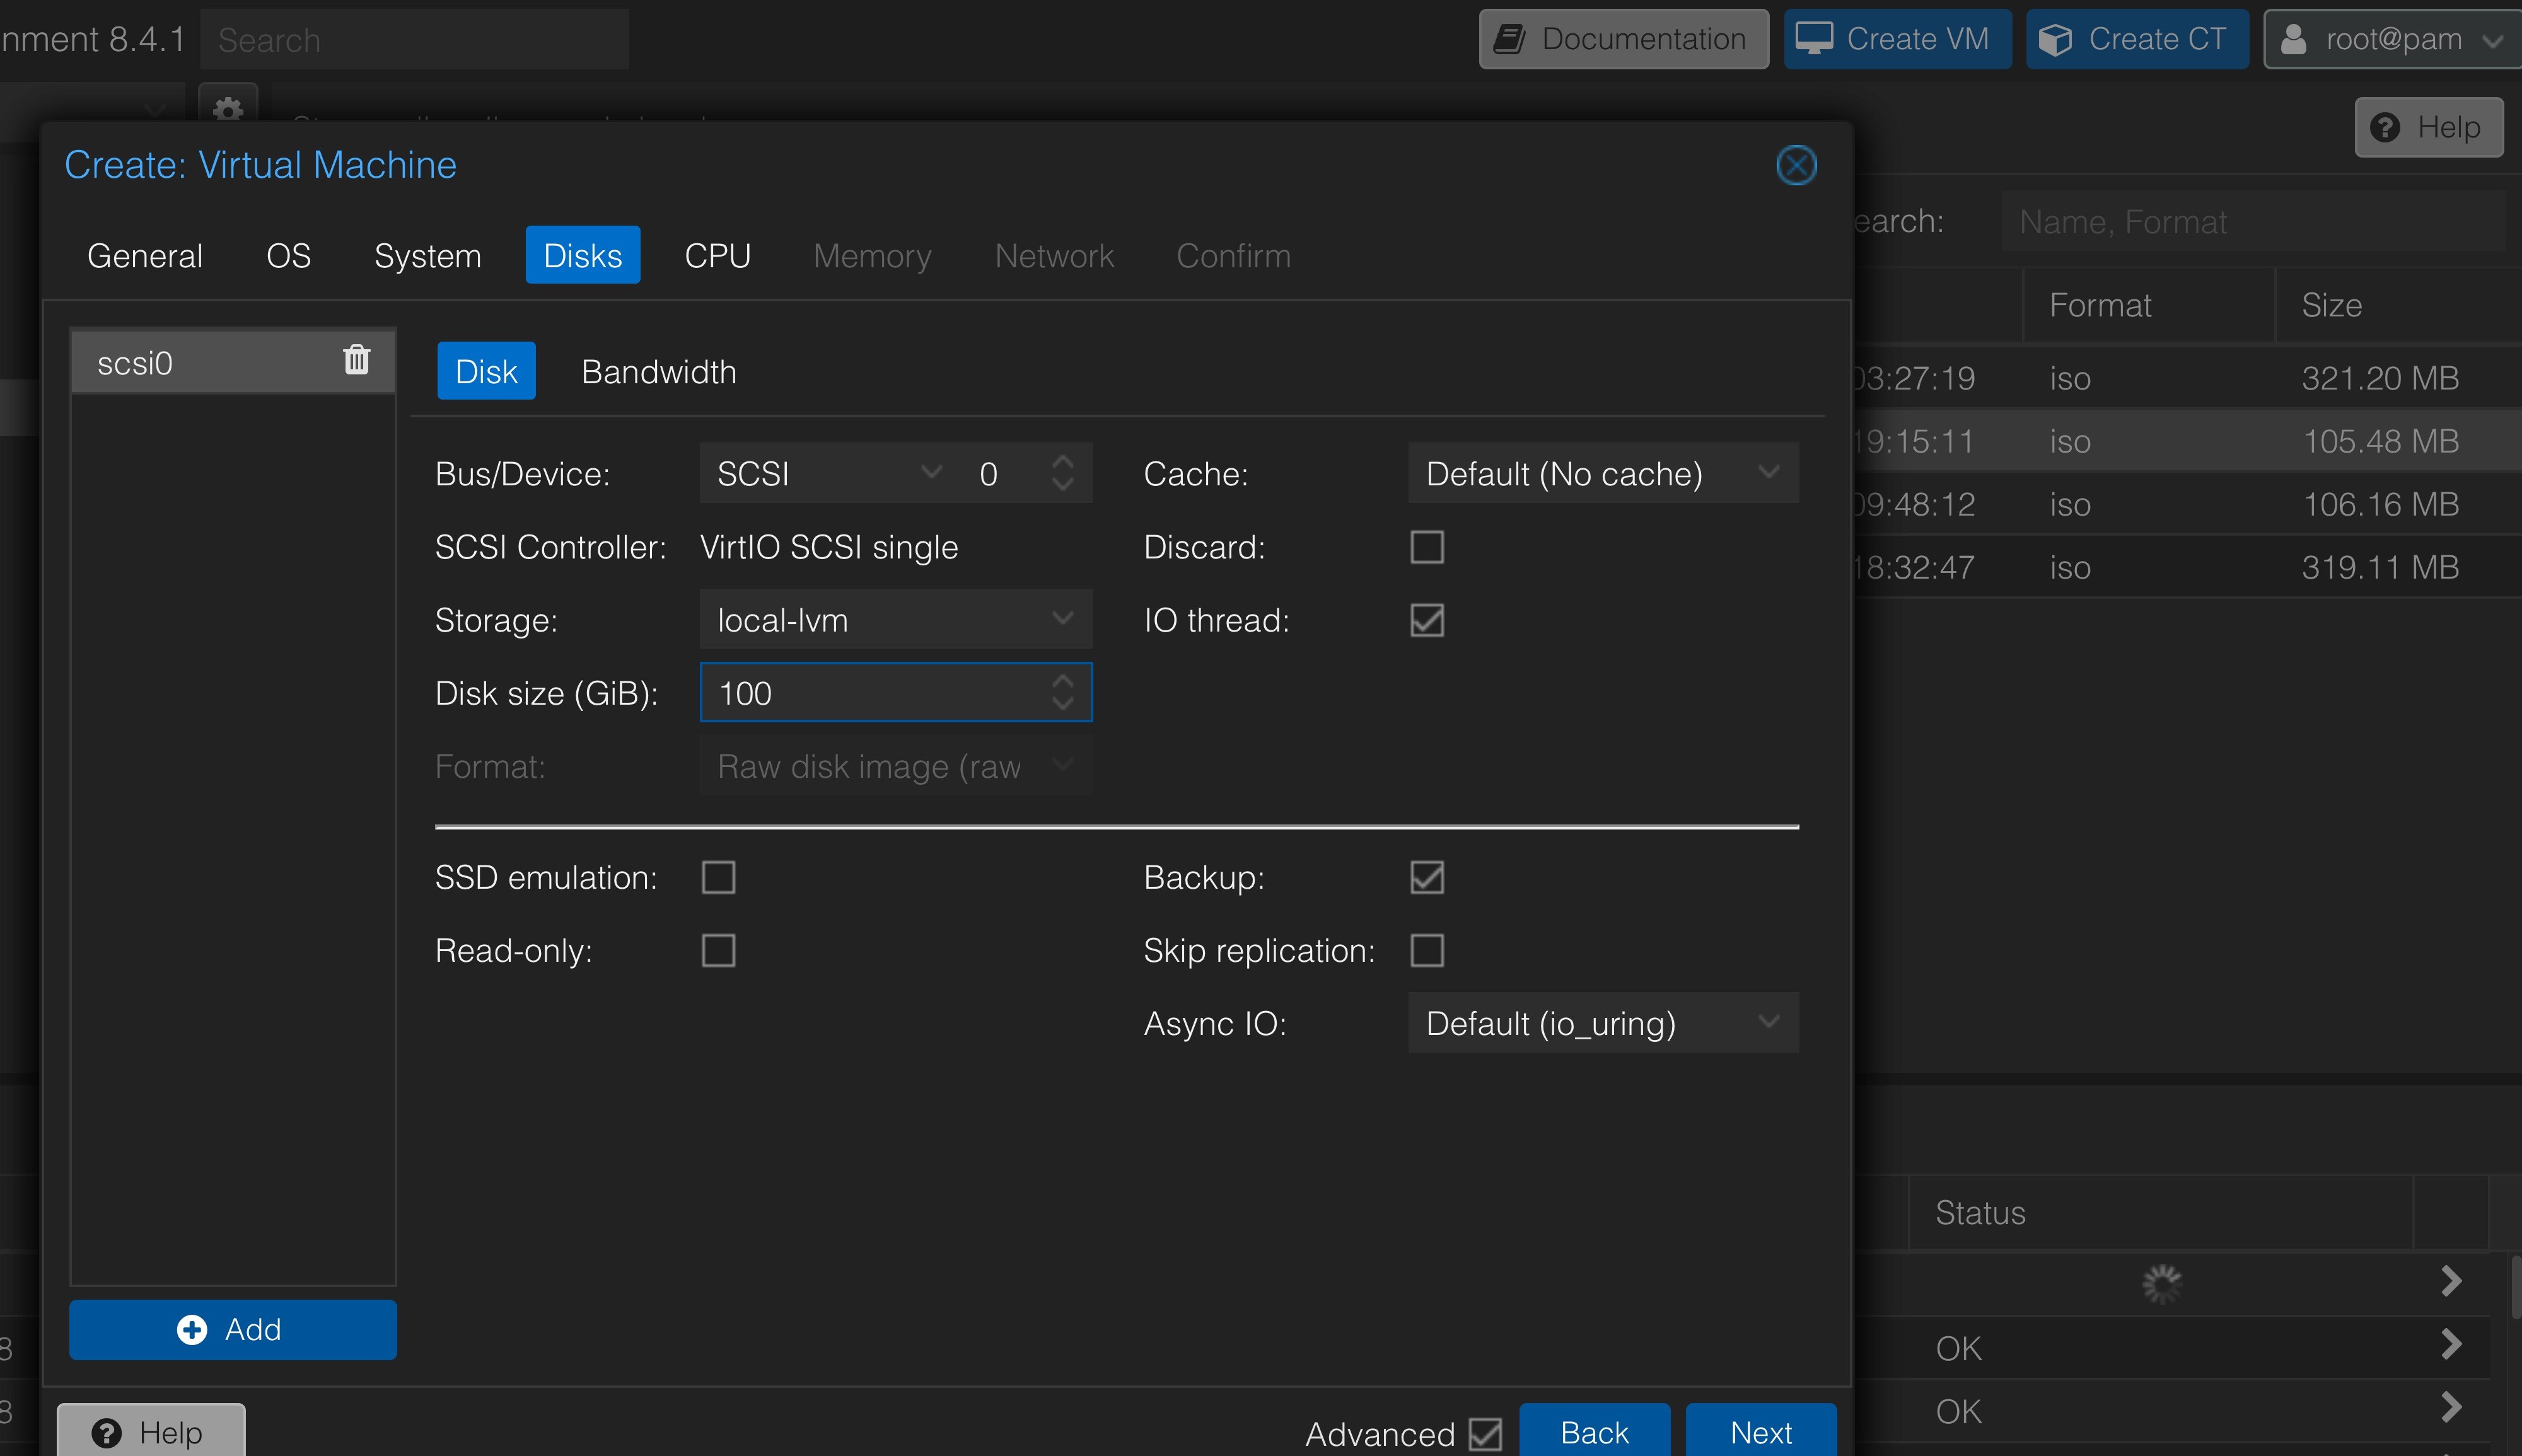
\includegraphics[width=1\textwidth]{figures/talos-install-5.jpg}
  \caption{Instalasi Talos OS 4}
  \label{fig:talos_install_4}
\end{figure}
\begin{figure}[!htbp]
  5. Pada bagian CPU. Cukup merubah cores menjadi 2 atau 4 sesuai spesifikasi mesin yang diinginkan
  \centering
  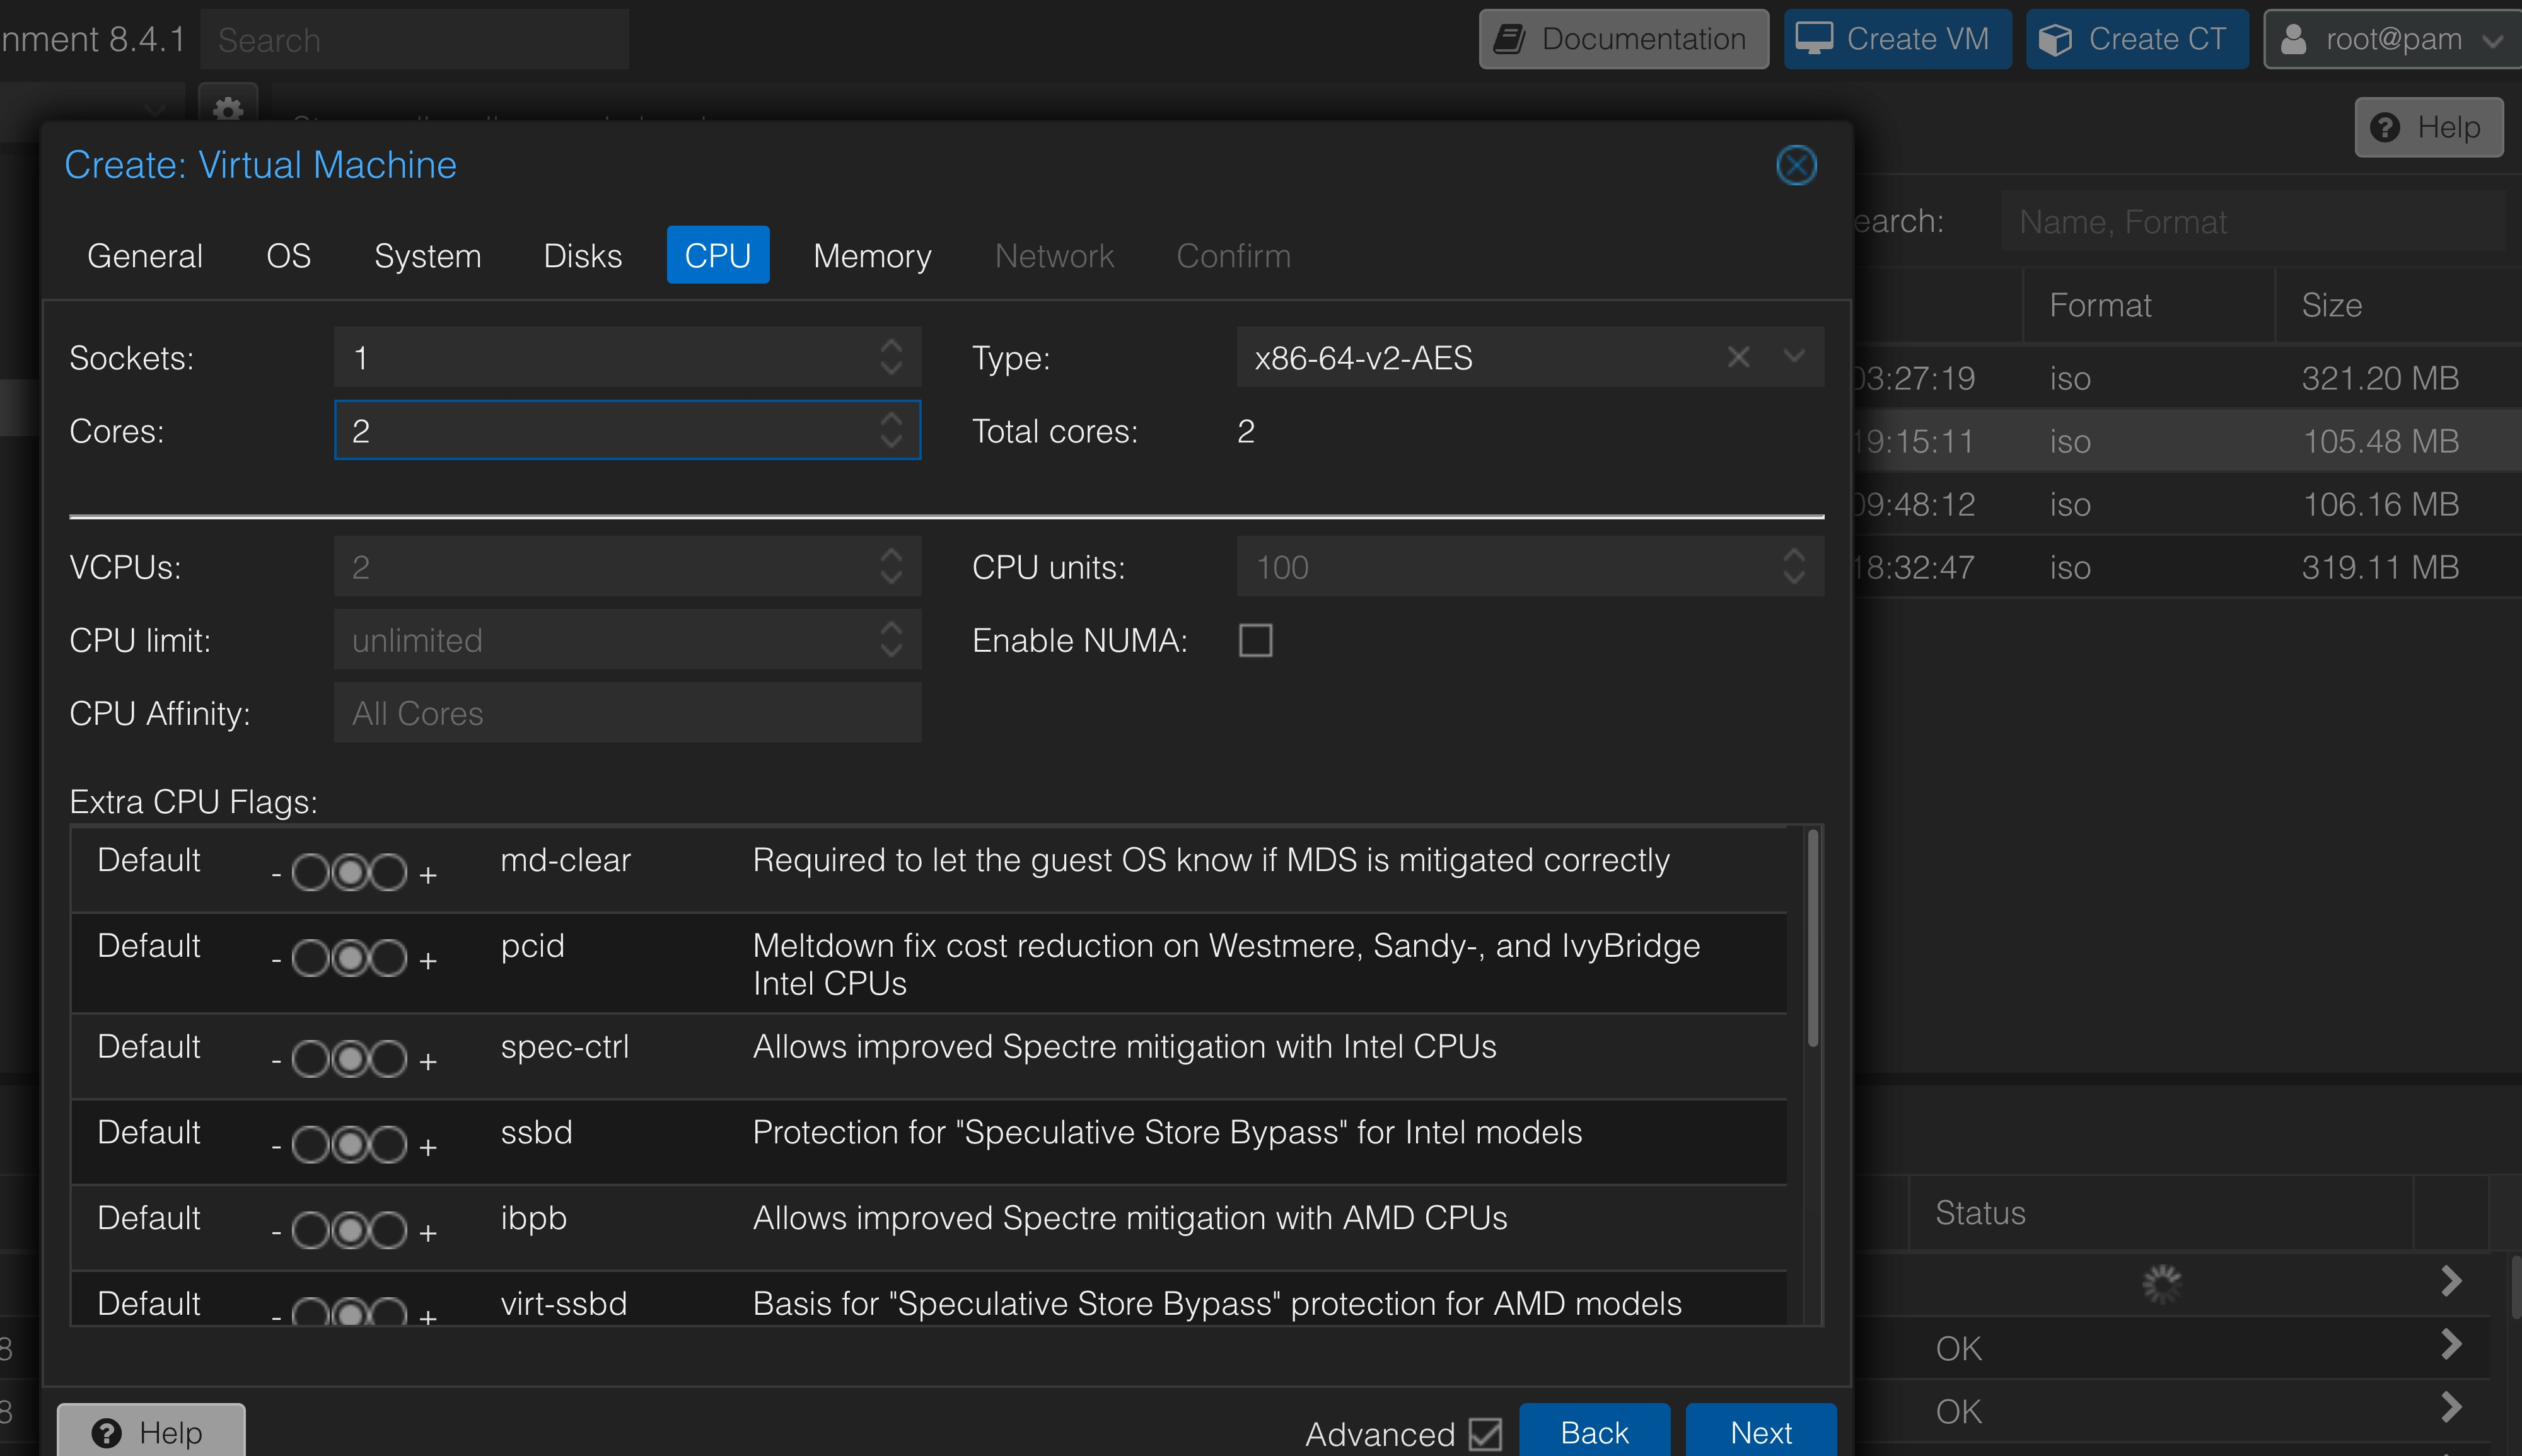
\includegraphics[width=1\textwidth]{figures/talos-install-6.jpg}
  \caption{Instalasi Talos OS 5}
  \label{fig:talos_install_5}
\end{figure}
\begin{figure}[!htbp]
  6. Pada bagian memory. Isikan memory sesuai yang dinginkan dengan minimal 8192 MiB
  \centering
  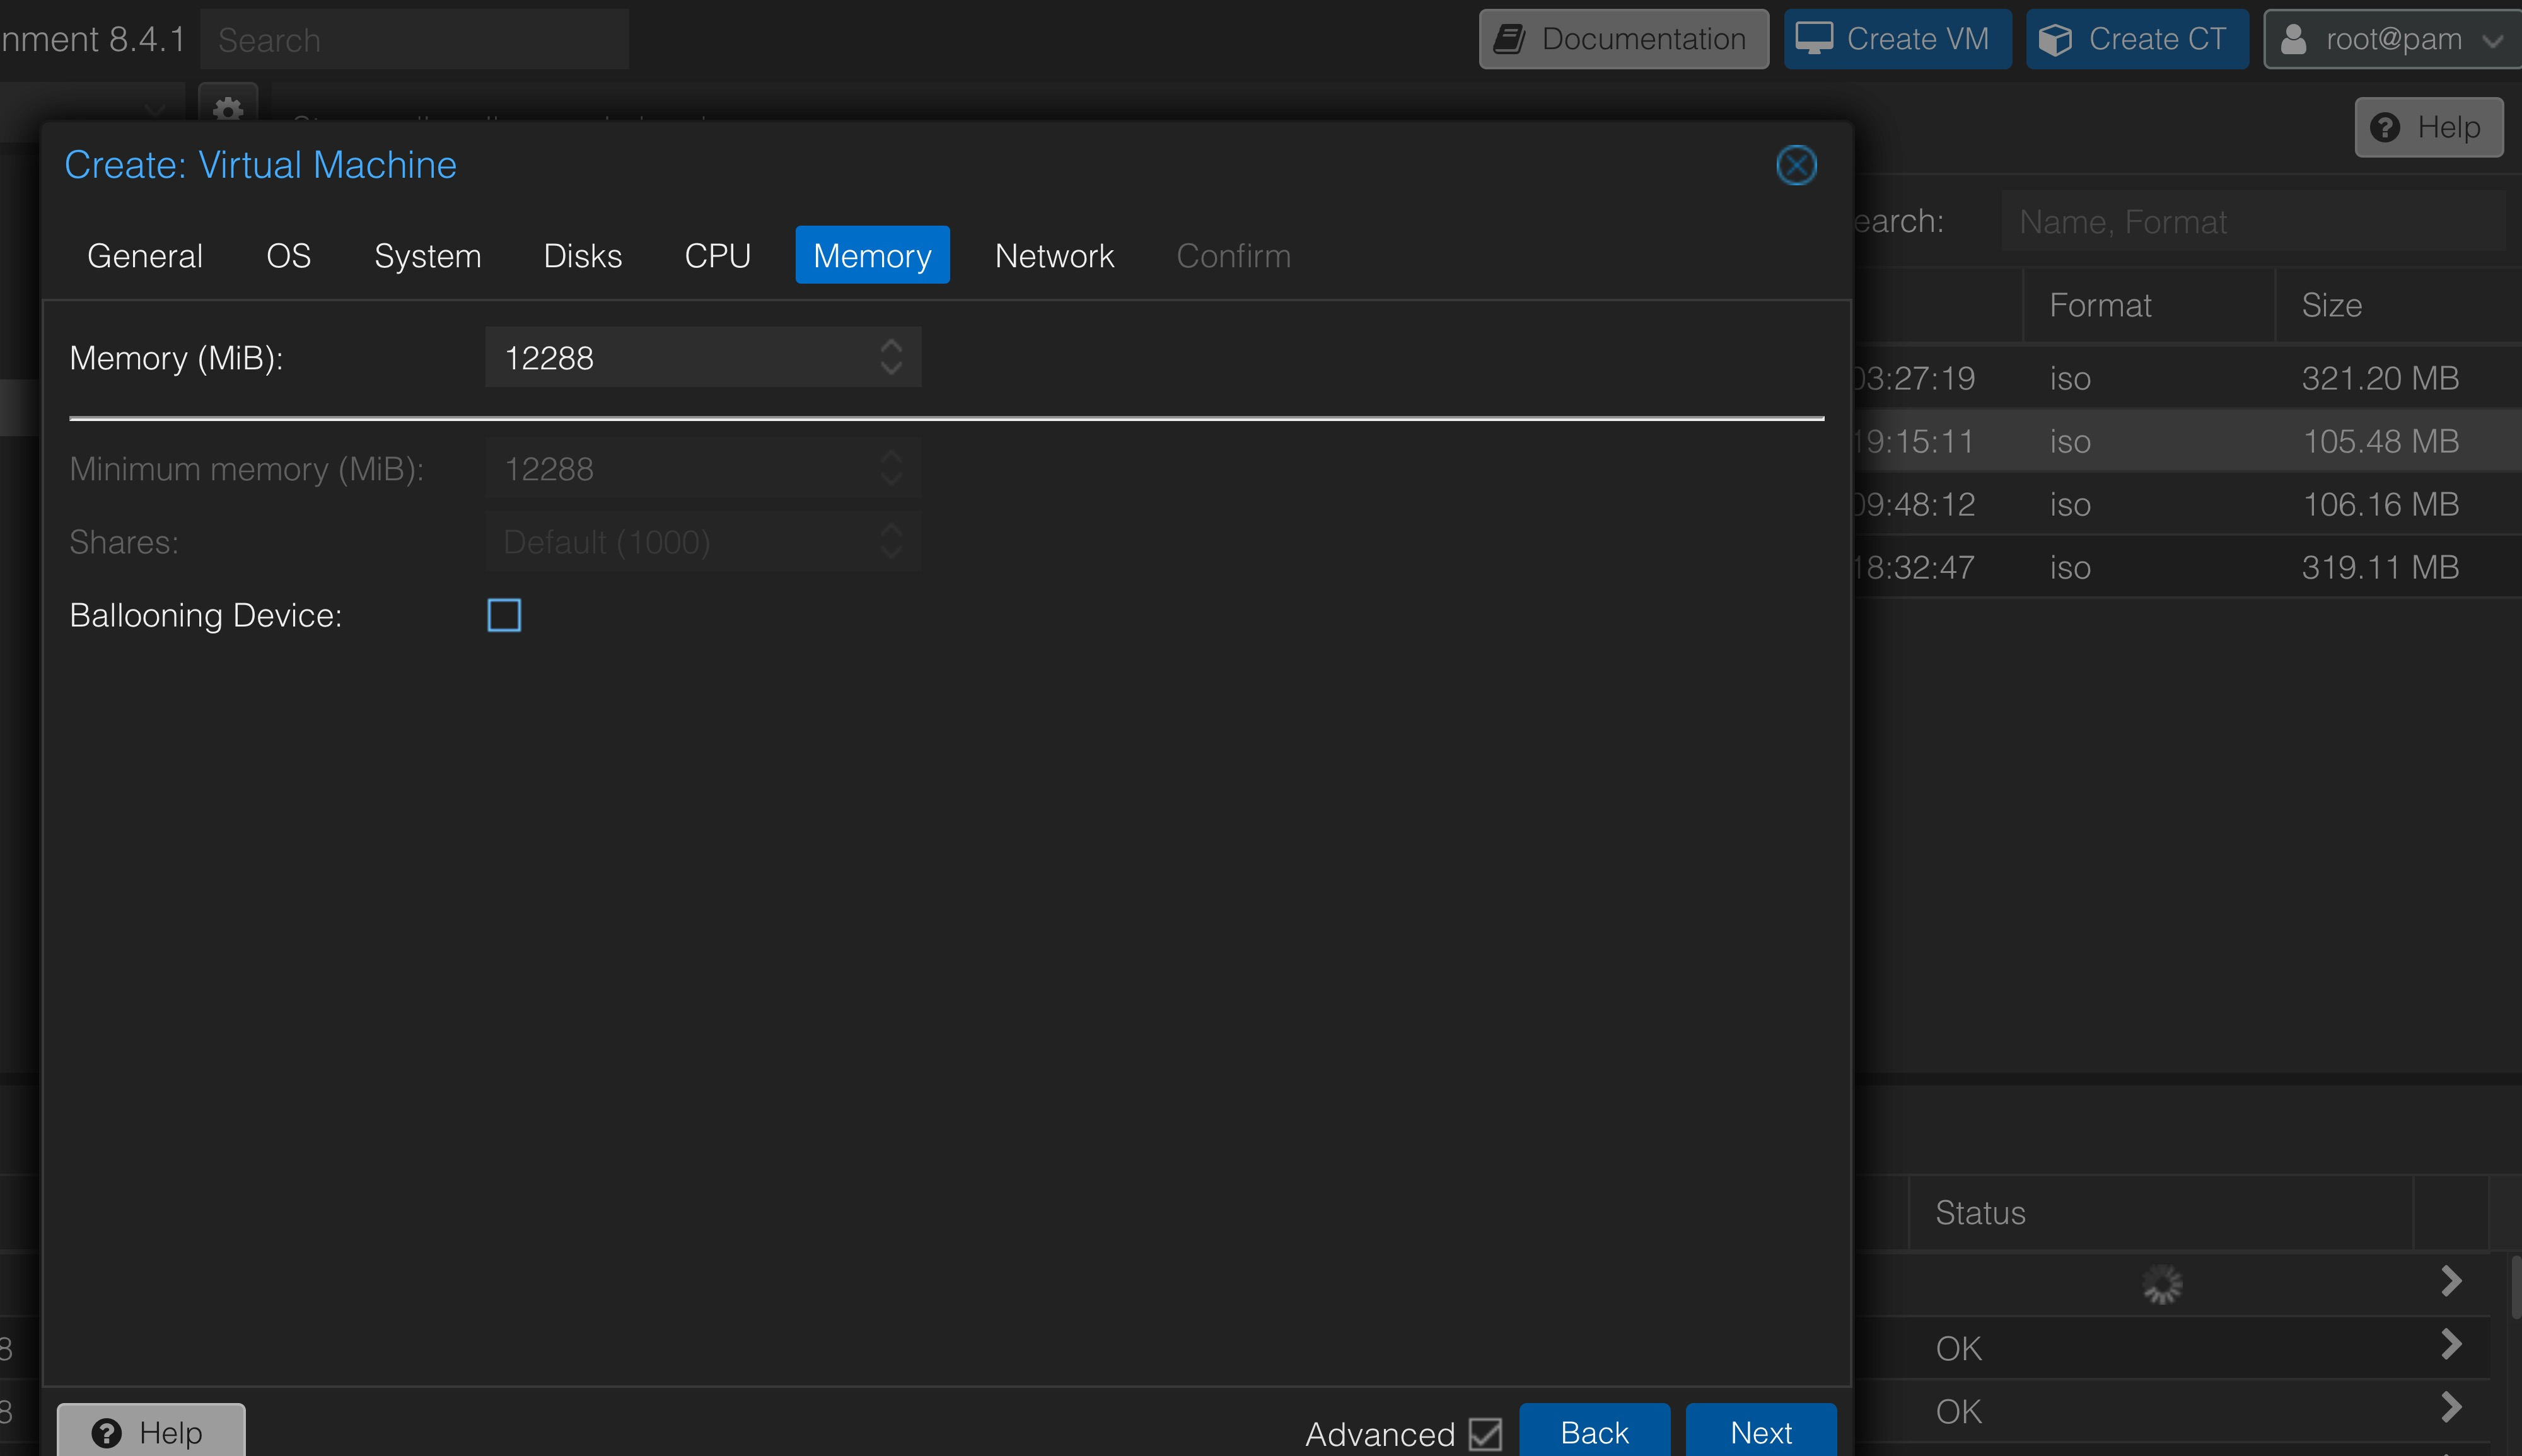
\includegraphics[width=1\textwidth]{figures/talos-install-7.jpg}
  \caption{Instalasi Talos OS 6}
  \label{fig:talos_install_6}
\end{figure}
\begin{figure}[!htbp]
  7. Pada bagian Network. Silahkan klik next
  \centering
  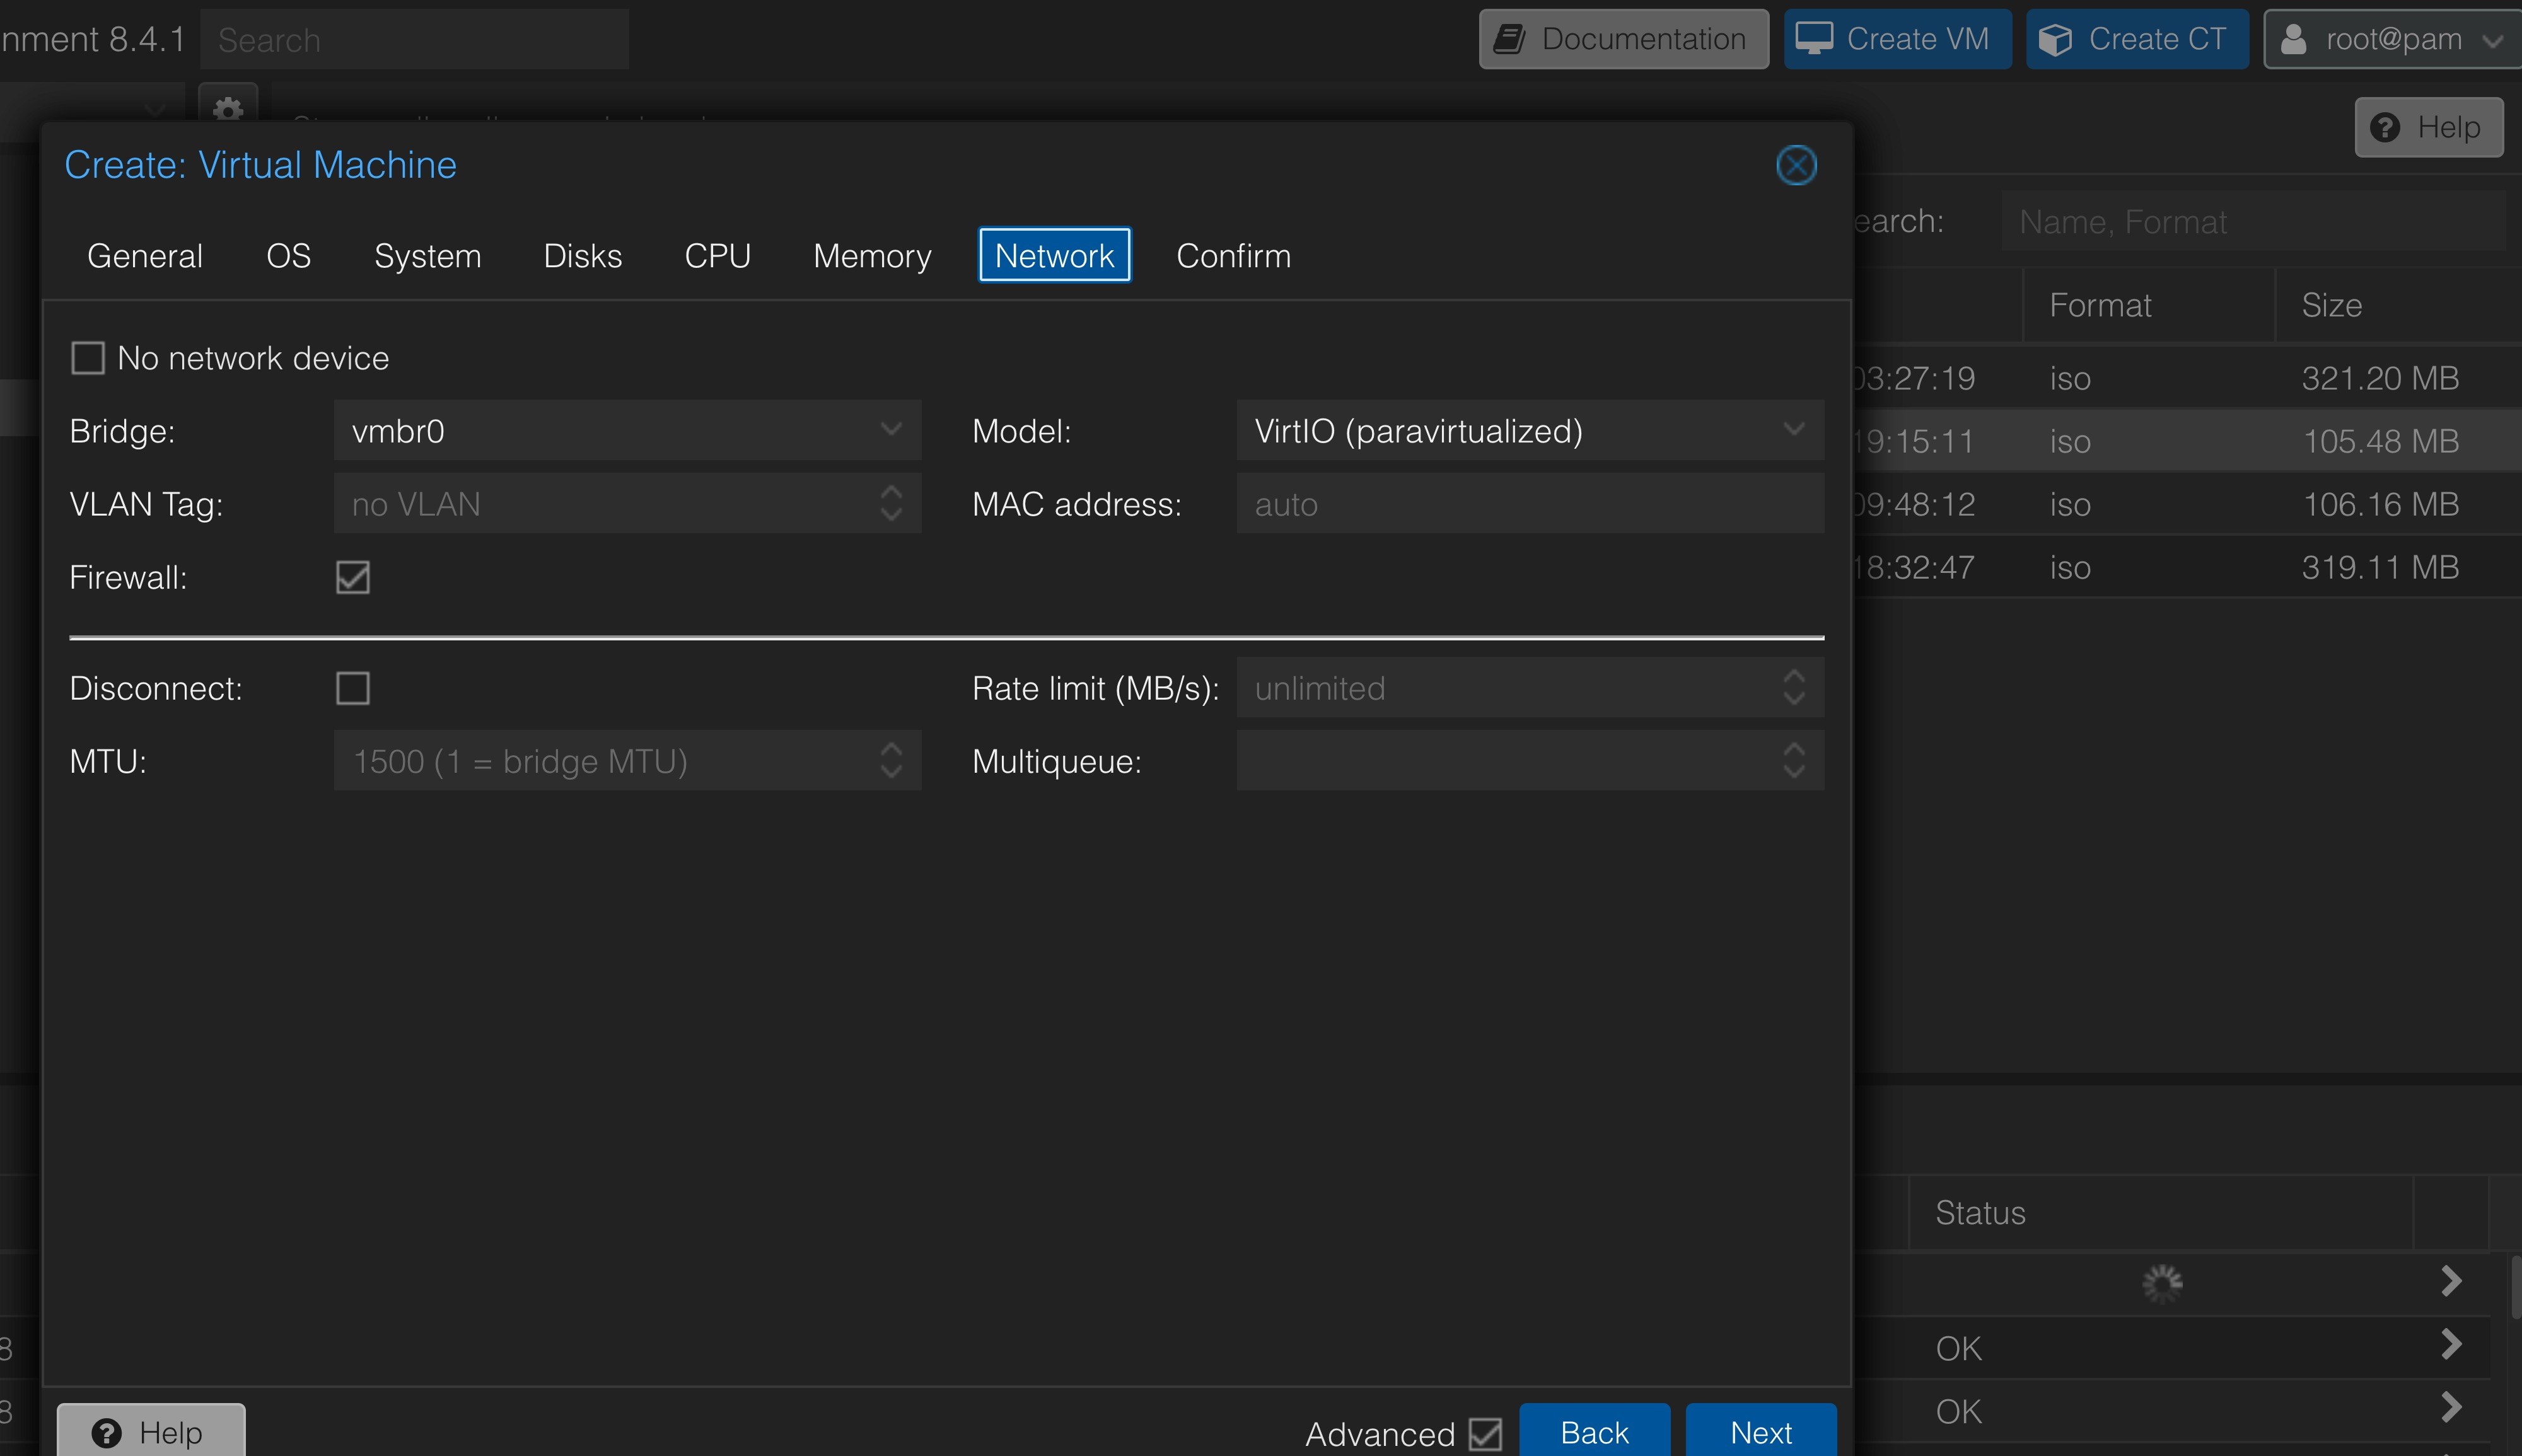
\includegraphics[width=1\textwidth]{figures/talos-install-8.jpg}
  \caption{Instalasi Talos OS 7}
  \label{fig:talos_install_7}
\end{figure}
\begin{figure}[!htbp]
  8. Pada bagian confirm. Centang "Start After Created" lalu Finish
  \centering
  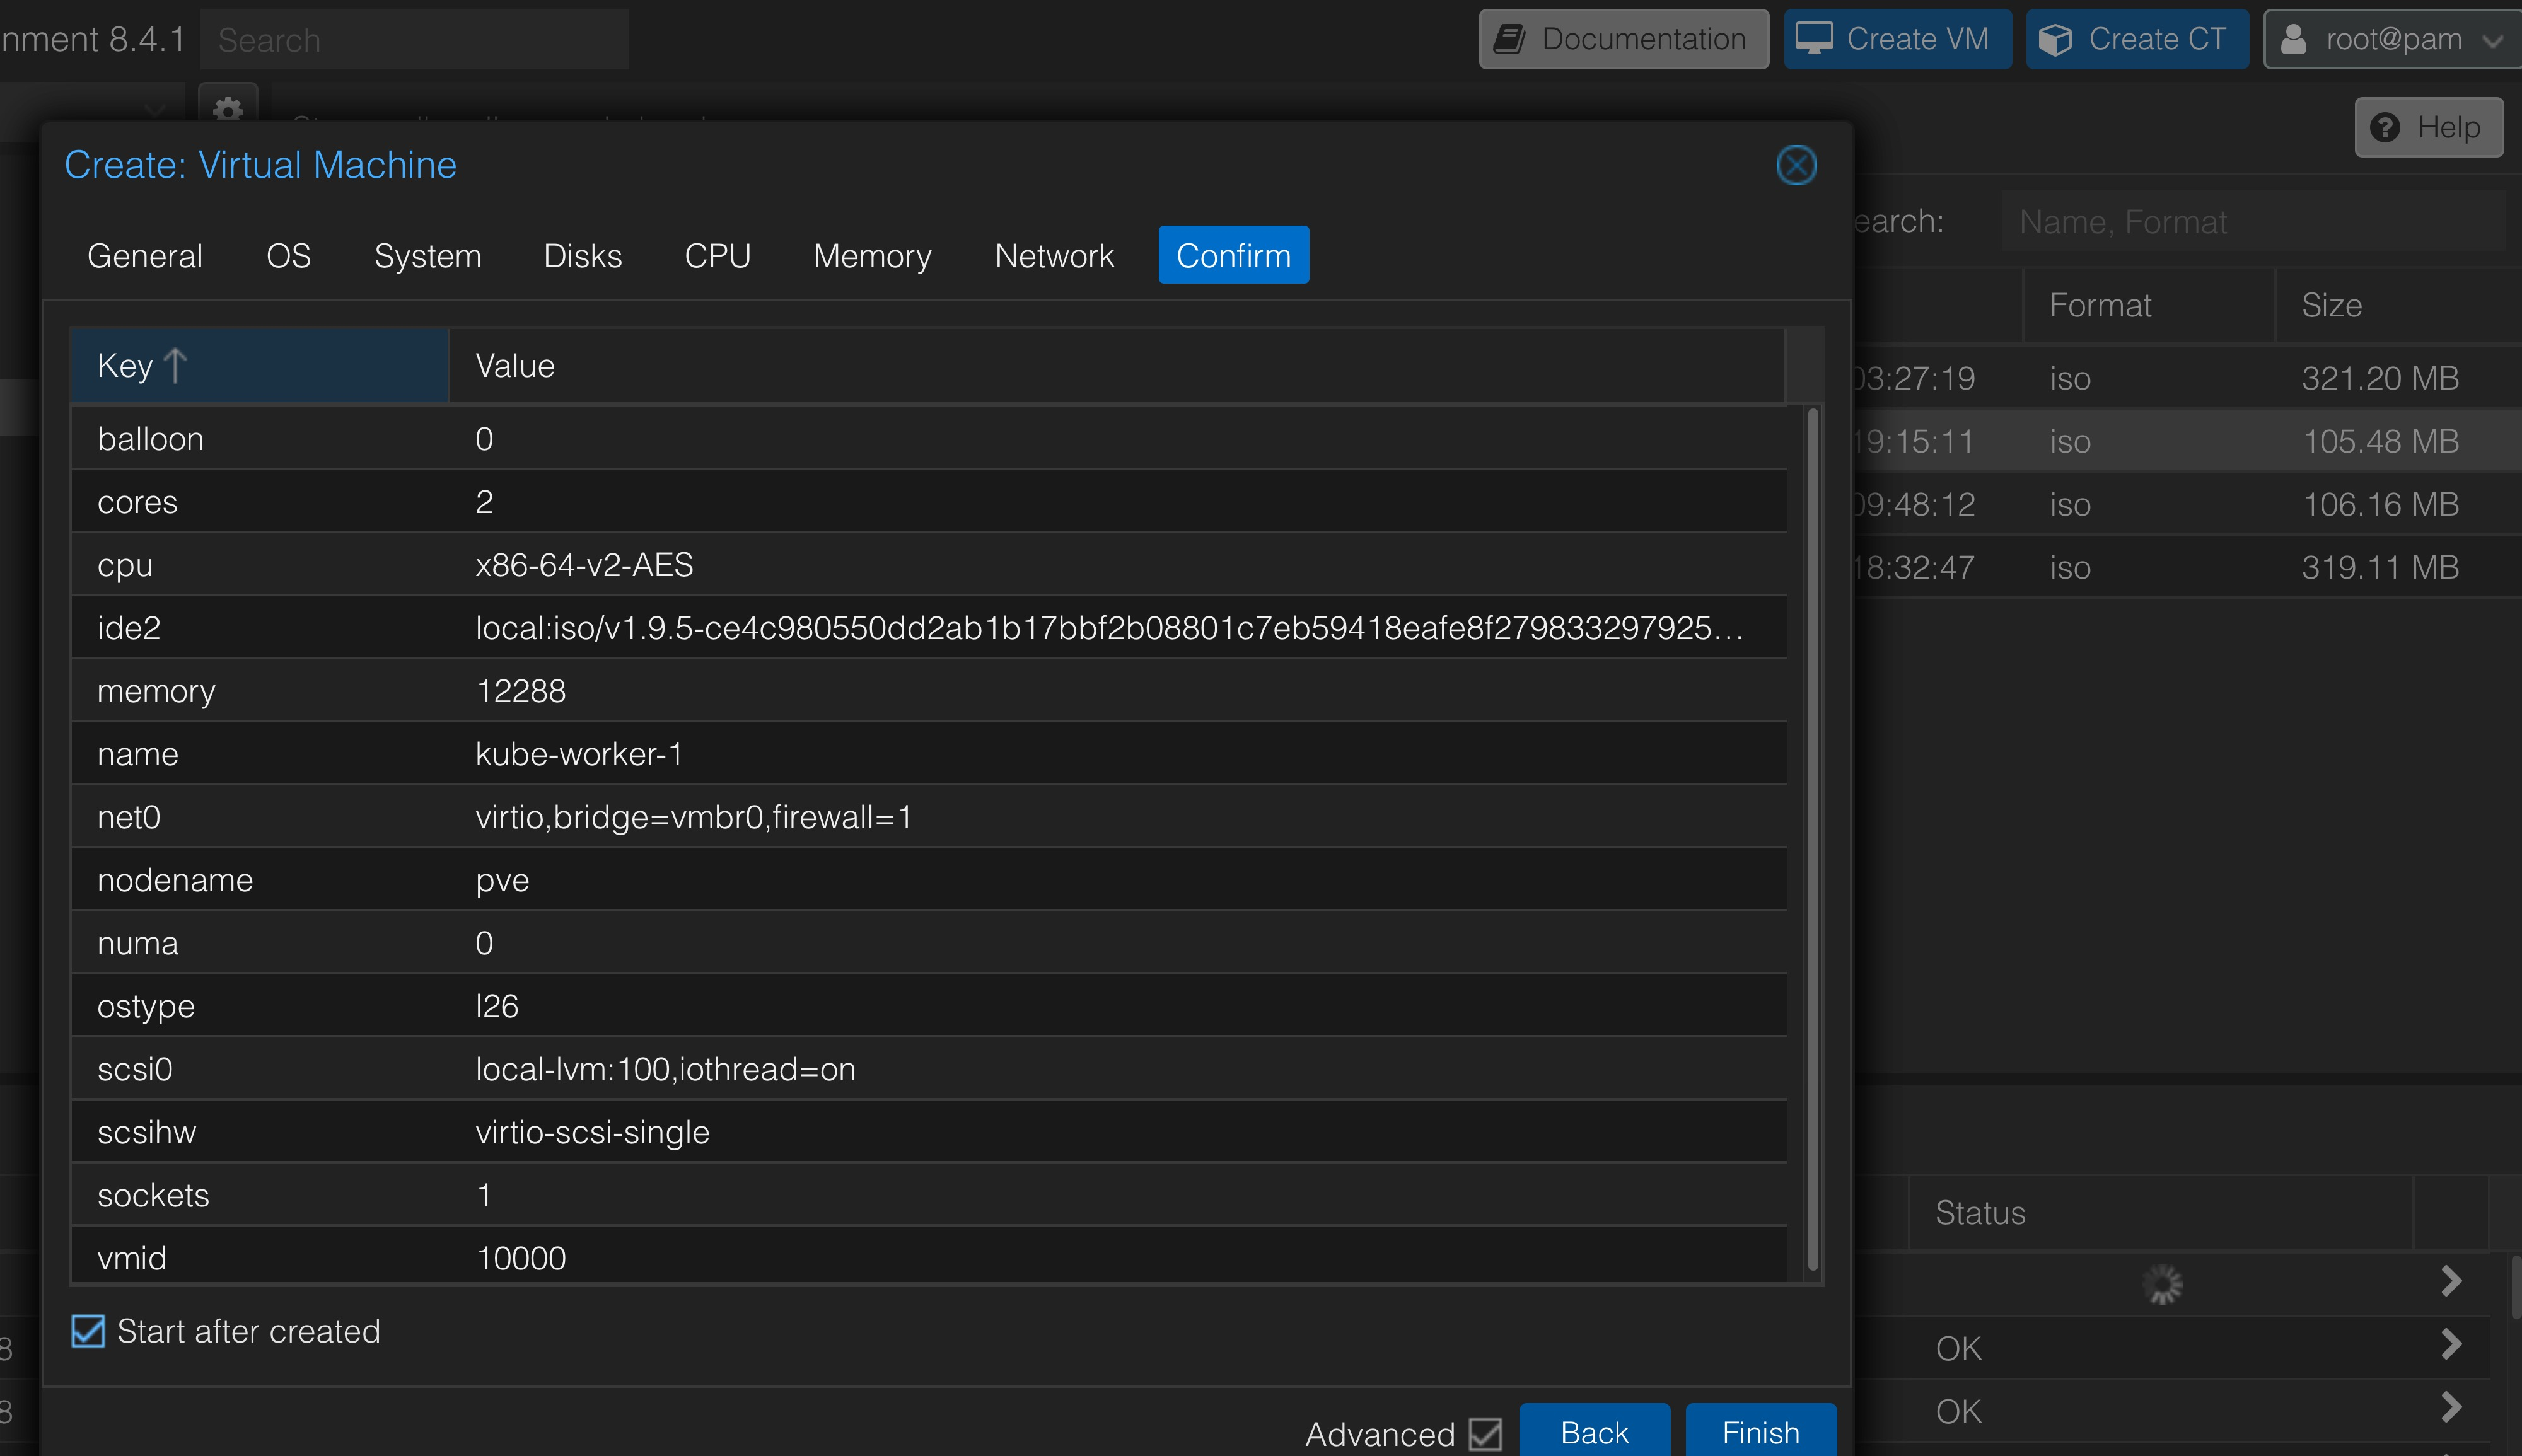
\includegraphics[width=1\textwidth]{figures/talos-install-9.jpg}
  \caption{Instalasi Talos OS 8}
  \label{fig:talos_install_8}
\end{figure}
\begin{figure}[!htbp]
  10. Ketika Talos OS Sudah berjalan terminal Talos OS akan tampak seperti ini
  \centering
  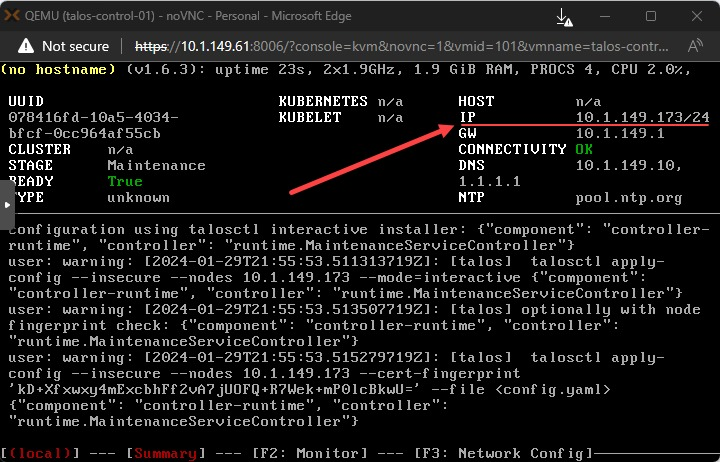
\includegraphics[width=1\textwidth]{figures/talos-install-10.jpg}
  \caption{Instalasi Talos OS 9}
  \label{fig:talos_install_9}
\end{figure}
\newpage
\subsubsection{Implementasi Instalasi Kubernetes pada Talos OS}
Tahap ini adalah tahap untuk instalasi Kubernetes pada Talos OS. Disini
peneliti akan menggunakan deklaratif yaml yang akan mengautomatisasi instalasi
kubernetes pada Talos OS. Instalasi Kubernetes pada Talos OS sendiri mengikuti
panduan dari pedoman yang terdapat pada website Talos OS
\url{https://www.talos.dev/v1.9.5/introduction/getting-started/}. \textbf{Kode
  Program \ref{lst:talos-cluster-config}} menunjukkan konfigurasi script
instalasi Kubernetes cluster pada Talos OS terdapat beberapa langkah yang akan
dijalankan yaitu dengan melakukan generate secret, generate config, generate
command apply, generate command bootstrap, dan generate command kubeconfig yang
akan digunakan sebagai konfigurasi dasar untuk instalasi Kubernetes cluster
pada Talos OS hasil dari generate config tersebut ditunjukan pada \textbf{Kode
  Program \ref{lst:talos-node-config}}.

\begin{lstlisting}[language=yaml, 
  basicstyle=\footnotesize\ttfamily, 
  caption={Konfigurasi script instalasi Kubernetes cluster pada Talos OS}, 
  label={lst:talos-cluster-config}]
version: '3'
tasks:
  talos:
    desc: Bootstrap the Talos cluster
    dir: '{{.TALOS_DIR}}'
    cmds:
      - '[ -f talsecret.sops.yaml ] || talhelper gensecret | sops --filename-override talos/talsecret.sops.yaml --encrypt /dev/stdin > talsecret.sops.yaml'
      - talhelper genconfig
      - talhelper gencommand apply --extra-flags="--insecure" | bash
      - until talhelper gencommand bootstrap | bash; do sleep 10; done
      - until talhelper gencommand kubeconfig --extra-flags="{{.ROOT_DIR}} --force" | bash; do sleep 10; done
\end{lstlisting}
\begin{lstlisting}[language=yaml, 
  basicstyle=\footnotesize\ttfamily, 
  caption={Konfigurasi node Kubernetes cluster pada Talos OS}, 
  label={lst:talos-node-config}]
clusterName: kubernetes
endpoint: https://192.168.0.250:6443
...
nodes:
  - hostname: "kube-cp-1"
    ipAddress: "192.168.0.200"
    installDisk: "/dev/sda"
    machineSpec:
    controlPlane: true
    networkInterfaces:
      - deviceSelector:
          hardwareAddr: "de:ad:be:ef:00:01"
        addresses:
          - "192.168.0.200/24"
        routes:
          - network: "0.0.0.0/0"
            gateway: "192.168.0.1"
        mtu: 1500
        vip:
          ip: "192.168.0.250"
  - hostname: "kube-worker-1"
    ipAddress: "192.168.0.201"
    installDisk: "/dev/sda"
    machineSpec:
    controlPlane: false
    networkInterfaces:
      - deviceSelector:
          hardwareAddr: "de:ad:be:ef:00:02"
        dhcp: false
        addresses:
          - "192.168.0.201/24"
        routes:
          - network: "0.0.0.0/0"
            gateway: "192.168.0.1"
        mtu: 1500
\end{lstlisting}

Setelah dilakukan instalasi Kubernetes cluster pada Talos OS tampilan terminal
akan menampilkan nama cluster dan juga sudah tidak menampilan status Stage:
Maintenance melainkan sudah menampilkan Kubelet: Healthy seperti \textbf{Gambar
  \ref{fig:talos_install_11}}.

\begin{figure}[!ht]
  \centering
  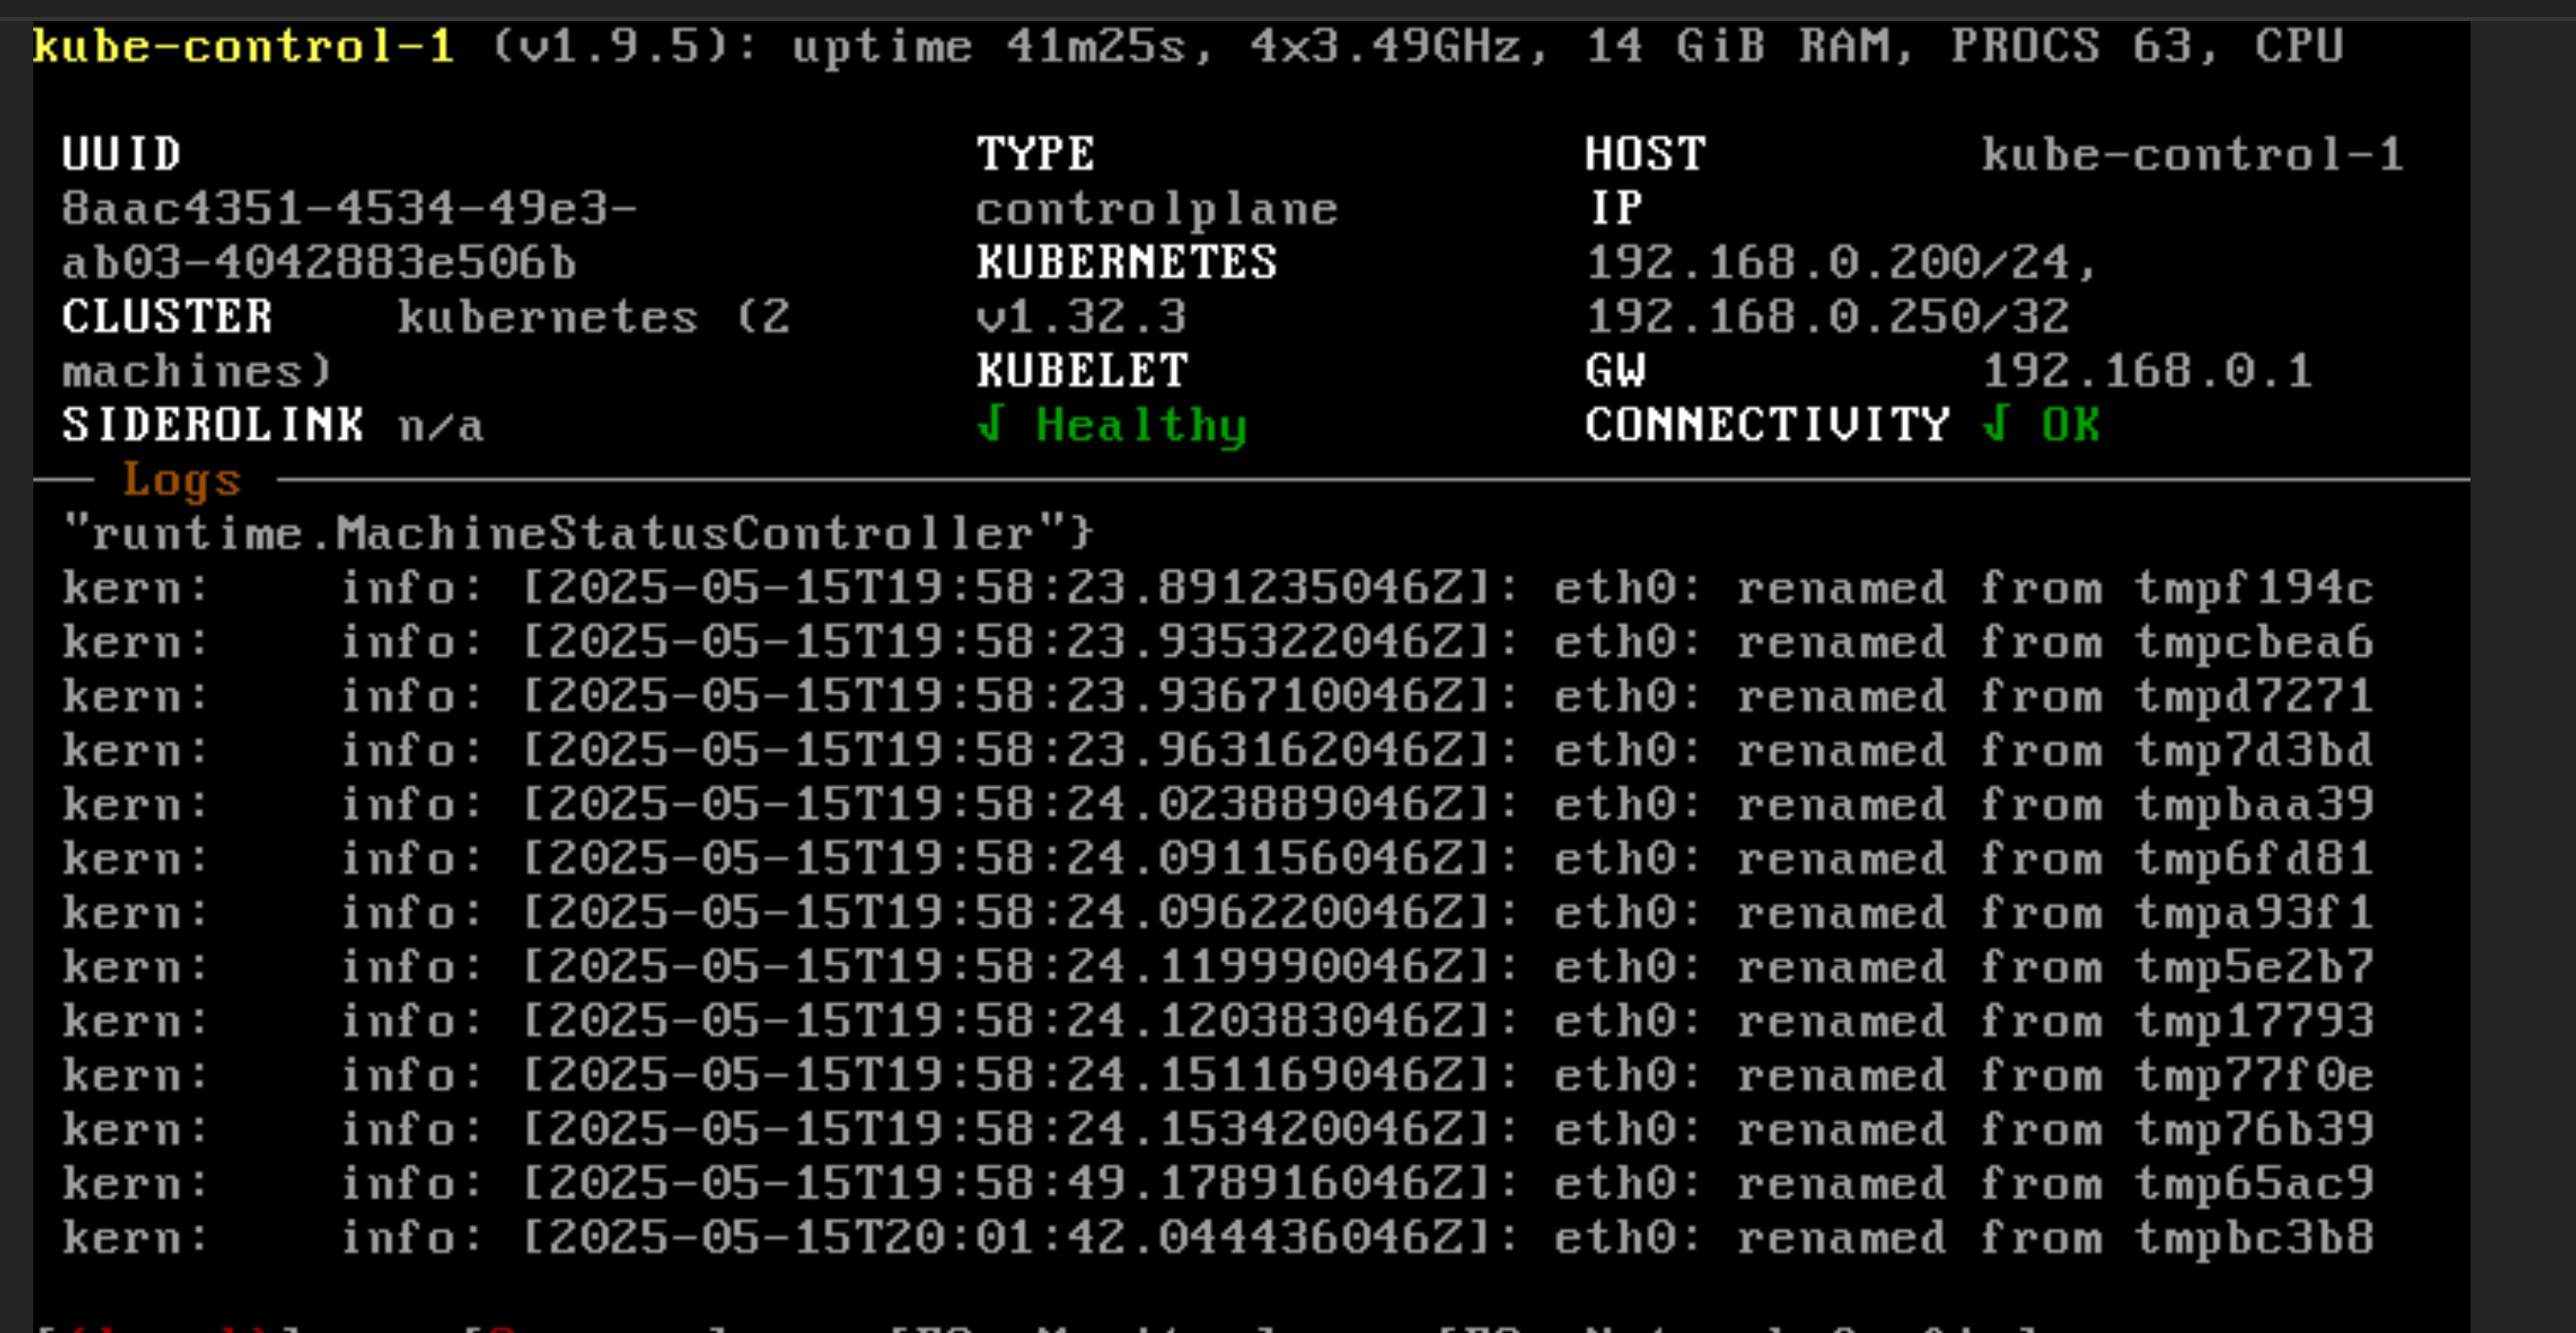
\includegraphics[width=1\textwidth]{figures/talos-install-11.jpg}
  \caption{Tampilan Talos OS setelah instalasi kubernetes cluster}
  \label{fig:talos_install_11}
\end{figure}

Setelah instalasi kubernetes pada Talos OS dilakukan maka kita dapat mengakses
kubernetes cluster tersebut menggunakan cli kubectl. Sebagai contoh
\textbf{Gambar \ref{fig:echo_web}} adalah aplikasi dummy yang menampilkan
informasi header pada browser pada \url{echo.zeinfahrozi.my.id}.

\newpage
\begin{figure}[h]
  \centering
  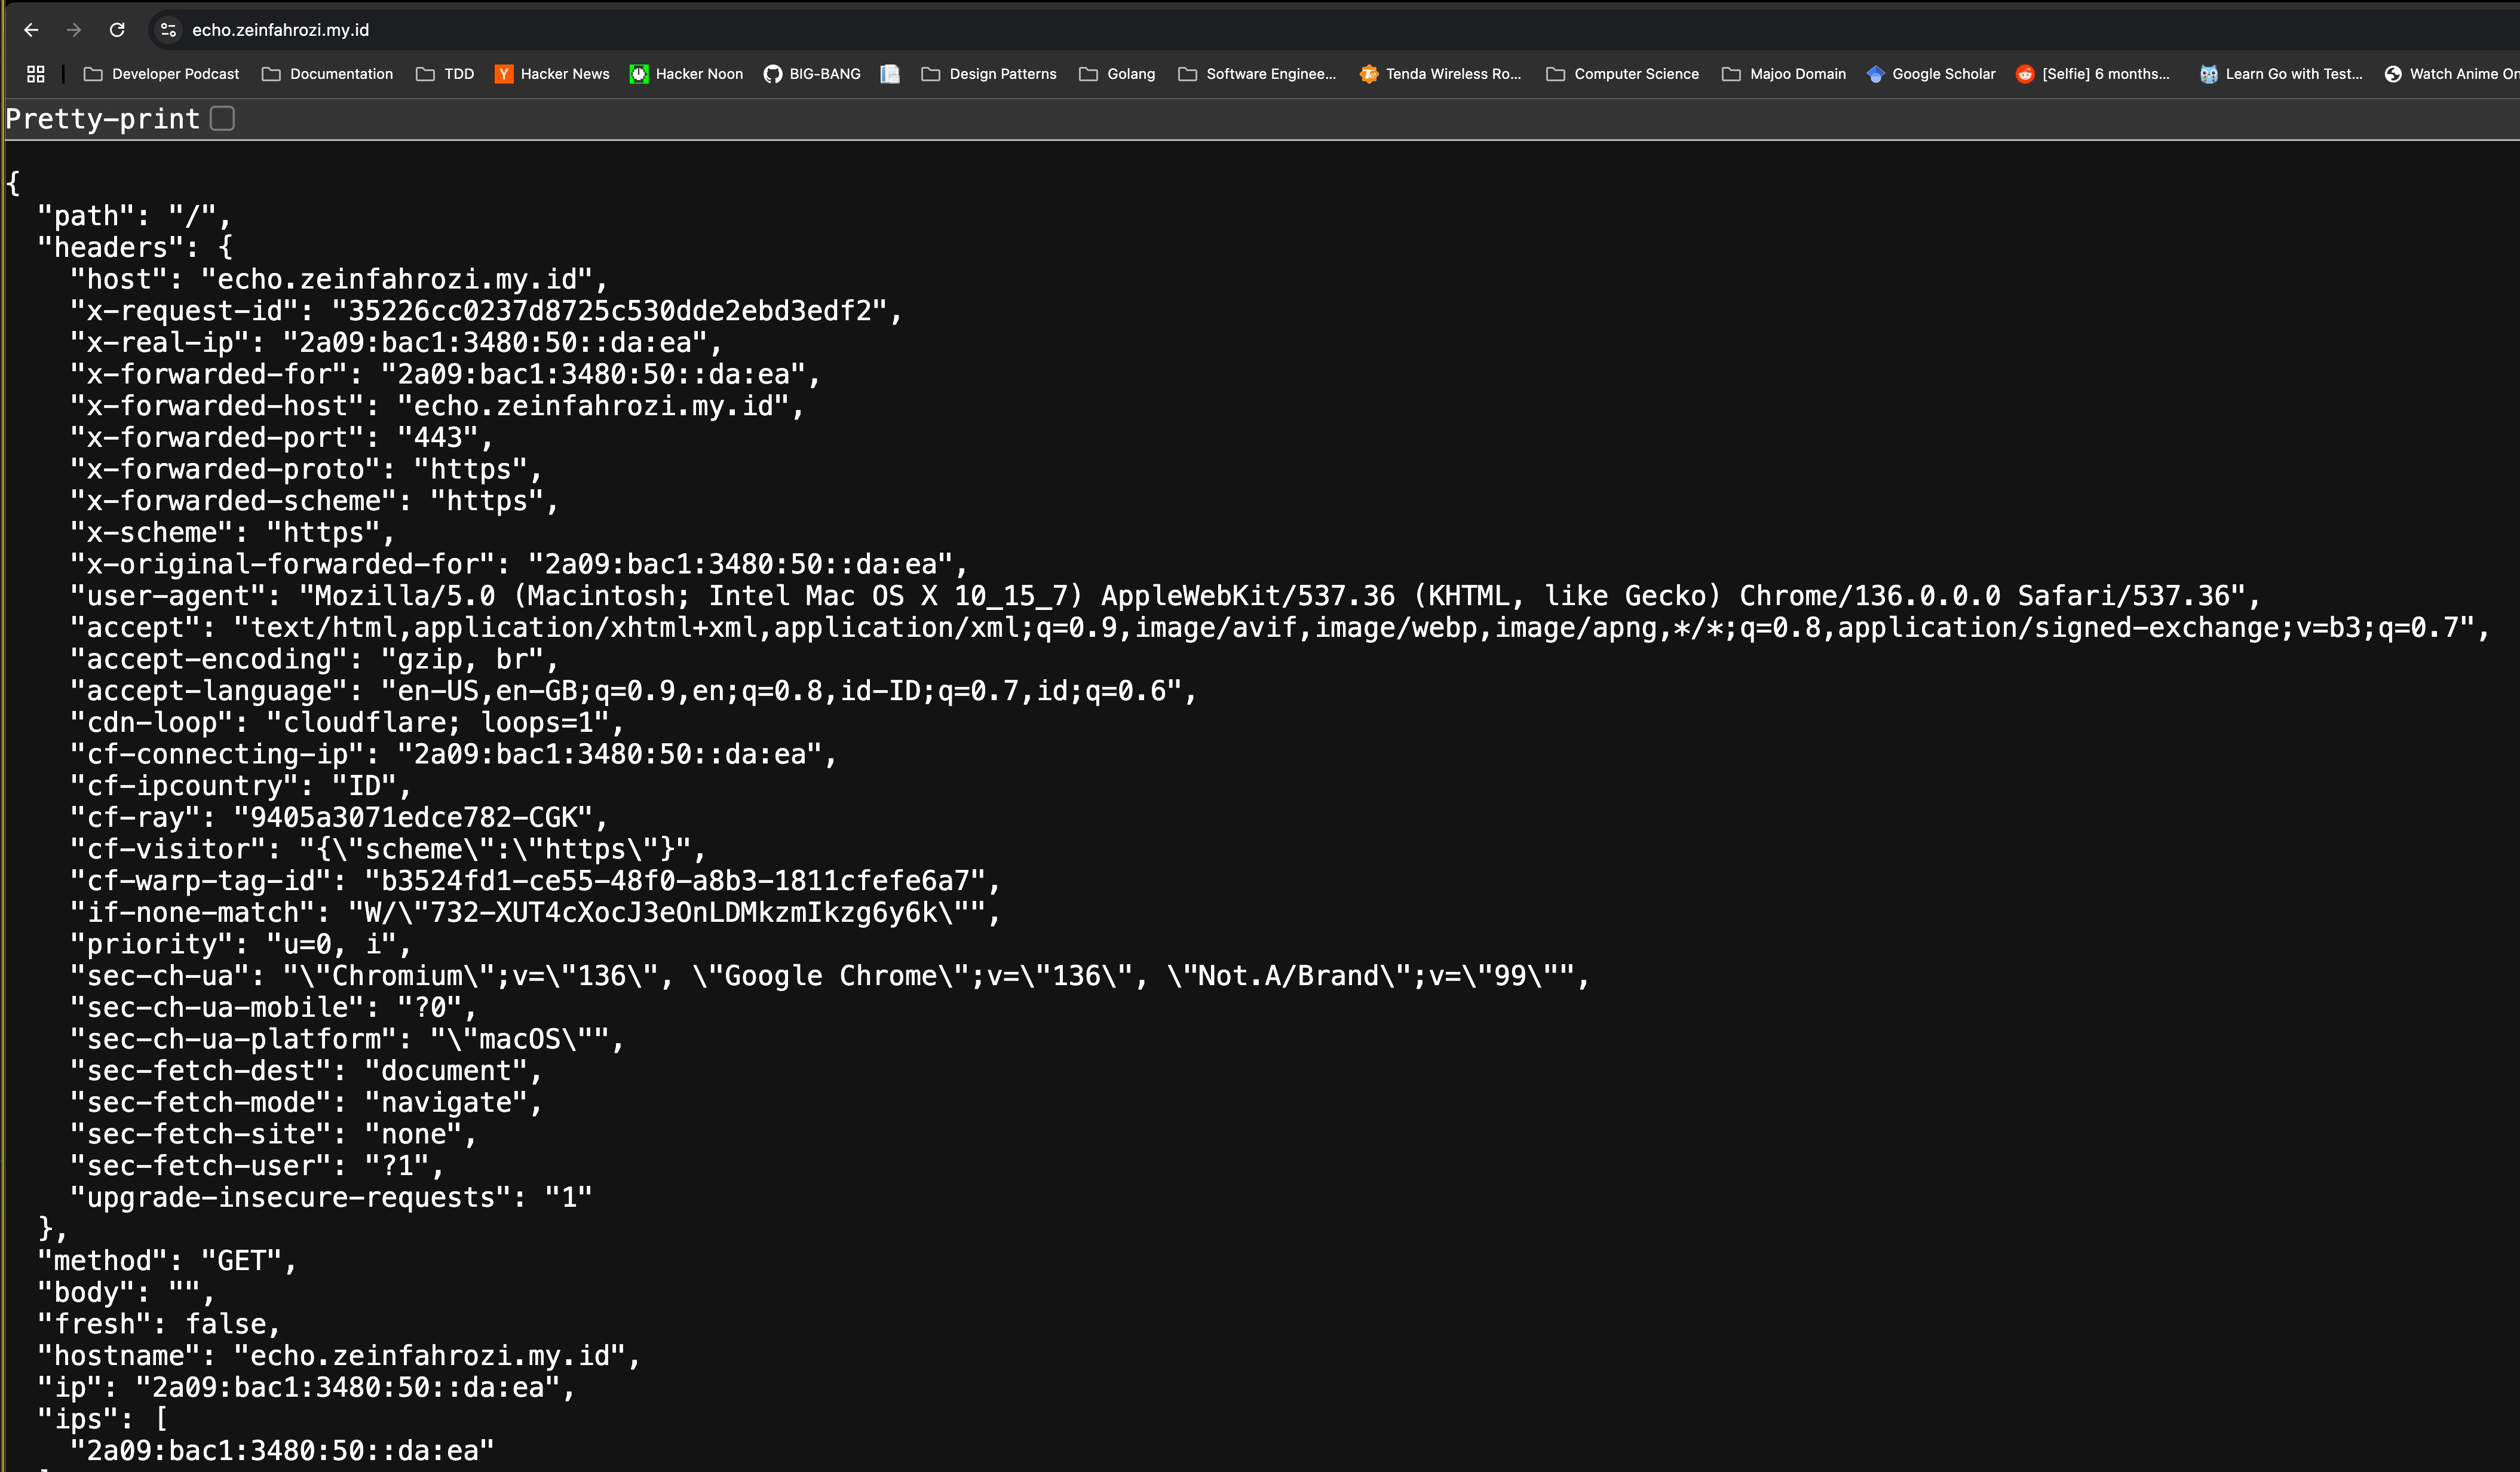
\includegraphics[width=1\textwidth]{figures/echo-web.jpg}
  \caption{Tampilan echo.zeinfahrozi.my.id pada browser}
  \label{fig:echo_web}
\end{figure}

\subsection{Implementasi ArgoCD pada Kubernetes Cluster}\label{sec:bab4_implementasi_argocd}
Tahap ini merupakan instalasi instance ArgoCD itu sendiri pada kubernetes
cluster yang sudah dibuat sebelumnya. ArgoCD dipasang menggunakan Helm chart
dengan konfigurasi kustom yang disesuaikan dengan kebutuhan lingkungan
produksi. Berikut adalah contoh perintah untuk menginstal ArgoCD menggunakan
Helm:

\begin{lstlisting}[language=bash, 
  basicstyle=\footnotesize\ttfamily,
  caption={Perintah Instalasi ArgoCD menggunakan Helm},
  label={lst:install-argocd}]
# Menambahkan repo ArgoCD
helm repo add argo https://argoproj.github.io/argo-helm
helm repo update

# Membuat namespace untuk ArgoCD
kubectl create namespace argocd

# Menginstal ArgoCD dengan Helm
helm upgrade --install argocd argo/argo-cd \
  --namespace argocd \
  --values values.sops.yaml \
  --wait
\end{lstlisting}

Pada \textbf{Kode Program \ref{lst:install-argocd}} menunjukkan perintah
instalasi ArgoCD menggunakan Helm charts dengan nilai-nilai kustom yang
didefinisikan dalam file \texttt{values.sops.yaml} yang ada pada \textbf{Kode
  Program \ref{lst:values-sops-yaml}}. Beberapa konfigurasi penting yang
diterapkan:

\begin{enumerate}[label=\alph*.]
  \item ArgoCD diakses melalui domain \texttt{argo.zeinfahrozi.my.id}
  \item Mode \texttt{insecure} diaktifkan untuk pengembangan
  \item Fitur status badge diaktifkan untuk memantau status aplikasi
  \item Dukungan untuk multiple value files dengan skema yang berbeda
  \item Eksklusi sumber daya tertentu seperti CiliumIdentity dari manajemen ArgoCD
\end{enumerate}

\begin{lstlisting}[language=yaml, 
  basicstyle=\footnotesize\ttfamily,
  caption={Contoh konfigurasi \texttt{values.sops.yaml} untuk ArgoCD},
  label={lst:values-sops-yaml}]
# values.sops.yaml
crds:
  install: true

global:
  domain: argo.zeinfahrozi.my.id

configs:
  params:
    server.insecure: true
  cm:
    statusbadge.enabled: true
    kustomize.buildOptions: --enable-alpha-plugins --enable-exec
    helm.valuesFileSchemes: >-
      secrets+gpg-import,secrets+gpg-import-kubernetes,
      secrets+age-import,secrets+age-import-kubernetes,
      secrets,secrets+literal,https
    resource.exclusions: |
      - apiGroups:
          - cilium.io
        kinds:
          - CiliumIdentity
        clusters:
          - "*"
\end{lstlisting}

Setelah ArgoCD terinstal, aplikasi-aplikasi dapat dikelola menggunakan GitOps.
Setiap aplikasi didefinisikan sebagai kustom resource Kubernetes yang
mereferensikan repositori Git yang berisi manifest Kubernetes. ArgoCD akan
secara otomatis melakukan sinkronisasi antara status yang diinginkan (yang
didefinisikan di Git) dengan status aktual di cluster. Beberapa aspek keamanan
yang diterapkan pada instalasi ArgoCD ini antara lain:

\begin{enumerate}[label=\alph*.]
  \item Penggunaan HTTPS untuk akses web UI
  \item Integrasi dengan Dex untuk autentikasi
  \item Pembatasan akses berbasis peran (RBAC)
  \item Penyimpanan rahasia yang aman menggunakan SOPS
\end{enumerate}

Dengan konfigurasi ini, ArgoCD siap digunakan untuk mengelola aplikasi secara
deklaratif menggunakan prinsip GitOps, di mana semua perubahan konfigurasi
dilakukan melalui pull request dan version control system.

\subsubsection{Implementasi Cloudflare Tunnel}
Cloudflare Tunnel digunakan untuk mengekspos layanan dalam cluster ke internet
dengan aman tanpa perlu membuka port firewall. Berikut adalah langkah-langkah
implementasinya:

Sebelum memulai implementasi, pastikan beberapa hal berikut sudah disiapkan:
\begin{itemize}
  \item Memiliki akun Cloudflare
  \item Mendaftarkan domain yang akan digunakan
  \item Mengatur DNS di Cloudflare
\end{itemize}

Cloudflare Tunnel diinstal menggunakan ArgoCD dengan konfigurasi seperti yang
ditunjukkan pada \textbf{Kode Program \ref{lst:cloudflared-argocd}}. Beberapa
konfigurasi penting dalam tabel tersebut antara lain:

\begin{itemize}
  \item \texttt{apiVersion} dan \texttt{kind}: Menentukan jenis resource Kubernetes yang akan dibuat, dalam hal ini adalah ArgoCD Application
  \item \texttt{metadata.name} dan \texttt{metadata.namespace}: Menentukan nama aplikasi (\texttt{cloudflared}) dan namespace tempat aplikasi akan di-deploy (\texttt{argo-system})
  \item \texttt{spec.project}: Menentukan project ArgoCD yang akan digunakan (\texttt{kubernetes})
  \item \texttt{spec.sources}: Mendefinisikan sumber konfigurasi aplikasi dari repository Git
        \begin{itemize}
          \item \texttt{repoURL}: URL repository Git yang berisi konfigurasi Cloudflare Tunnel
          \item \texttt{path}: Lokasi file konfigurasi dalam repository (\texttt{kubernetes/apps/network/cloudflared})
          \item \texttt{targetRevision}: Branch atau tag Git yang akan digunakan (\texttt{main})
        \end{itemize}
  \item \texttt{spec.destination}: Menentukan cluster dan namespace target untuk deployment
  \item \texttt{spec.syncPolicy.automated}: Mengaktifkan sinkronisasi otomatis dengan opsi:
        \begin{itemize}
          \item \texttt{prune: true}: Secara otomatis menghapus resource yang tidak lagi ada di Git
          \item \texttt{selfHeal: true}: Secara otomatis memperbaiki perubahan yang dibuat di luar ArgoCD
        \end{itemize}
\end{itemize}

\begin{lstlisting}[language=yaml, 
  basicstyle=\footnotesize\ttfamily,
  caption={Konfigurasi ArgoCD untuk instalasi Cloudflare Tunnel},
  label={lst:cloudflared-argocd}]
apiVersion: argoproj.io/v1alpha1
kind: Application
metadata:
  name: cloudflared
  namespace: argo-system
spec:
  project: kubernetes
  sources:
    - repoURL: "https://github.com/mozarik/zein-home-lab.git"
      path: kubernetes/apps/network/cloudflared
      targetRevision: main
  destination:
    name: in-cluster
    namespace: network
  syncPolicy:
    automated:
      prune: true
      selfHeal: true
\end{lstlisting}

Setelah terinstal, Cloudflare Tunnel perlu dikonfigurasi untuk meneruskan lalu
lintas ke layanan dalam cluster. Konfigurasi dasar untuk mengekspos ArgoCD
melalui Cloudflare Tunnel dapat dilihat pada \textbf{Kode Program
  \ref{lst:cloudflared-config}}. Berikut penjelasan konfigurasi utamanya:

\begin{itemize}
  \item \texttt{tunnel}: ID unik yang mengidentifikasi tunnel Cloudflare. Nilai \texttt{<tunnel-id>} diganti dengan ID tunnel yang didapat dari Cloudflare.
  \item \texttt{credentials-file}: Lokasi file kredensial yang berisi token otentikasi untuk mengakses akun Cloudflare.
  \item \texttt{ingress}: Mendefinisikan aturan routing untuk lalu lintas yang masuk:
        \begin{itemize}
          \item Aturan pertama mengarahkan permintaan dengan hostname
                \texttt{argo.zeinfahrozi.my.id} ke service ArgoCD di dalam cluster
                (\texttt{http://argocd-server.argocd.svc.cluster.local:80})
          \item Aturan terakhir (\texttt{http\_status:404}) berfungsi sebagai fallback untuk
                menampilkan error 404 jika tidak ada aturan yang cocok
        \end{itemize}
\end{itemize}

\begin{lstlisting}[language=yaml, 
  basicstyle=\footnotesize\ttfamily,
  caption={Konfigurasi dasar Cloudflare Tunnel untuk ArgoCD},
  label={lst:cloudflared-config}]
# config.yaml
tunnel: <tunnel-id>
credentials-file: /etc/cloudflared/credentials.json
ingress:
  - hostname: argo.zeinfahrozi.my.id
    service: http://argocd-server.argocd.svc.cluster.local:80
  - service: http_status:404
\end{lstlisting}

Setelah konfigurasi di atas diterapkan, Cloudflare Tunnel akan secara otomatis
membuat koneksi aman dari jaringan Cloudflare ke cluster Kubernetes. Layanan
ArgoCD dapat diakses melalui domain \texttt{argo.zeinfahrozi.my.id} dengan
enkripsi TLS end-to-end. Semua lalu lintas akan melewati jaringan Cloudflare
sehingga meningkatkan keamanan dan performa akses.

\subsubsection{Konfigurasi Git Repository}
Git repository digunakan sebagai sumber kebenaran (source of truth) untuk
konfigurasi infrastruktur. Repository yang digunakan adalah
\url{https://github.com/mozarik/zein-home-lab}.

\begin{figure}[H]
  \centering
  \fcolorbox{black}{white}{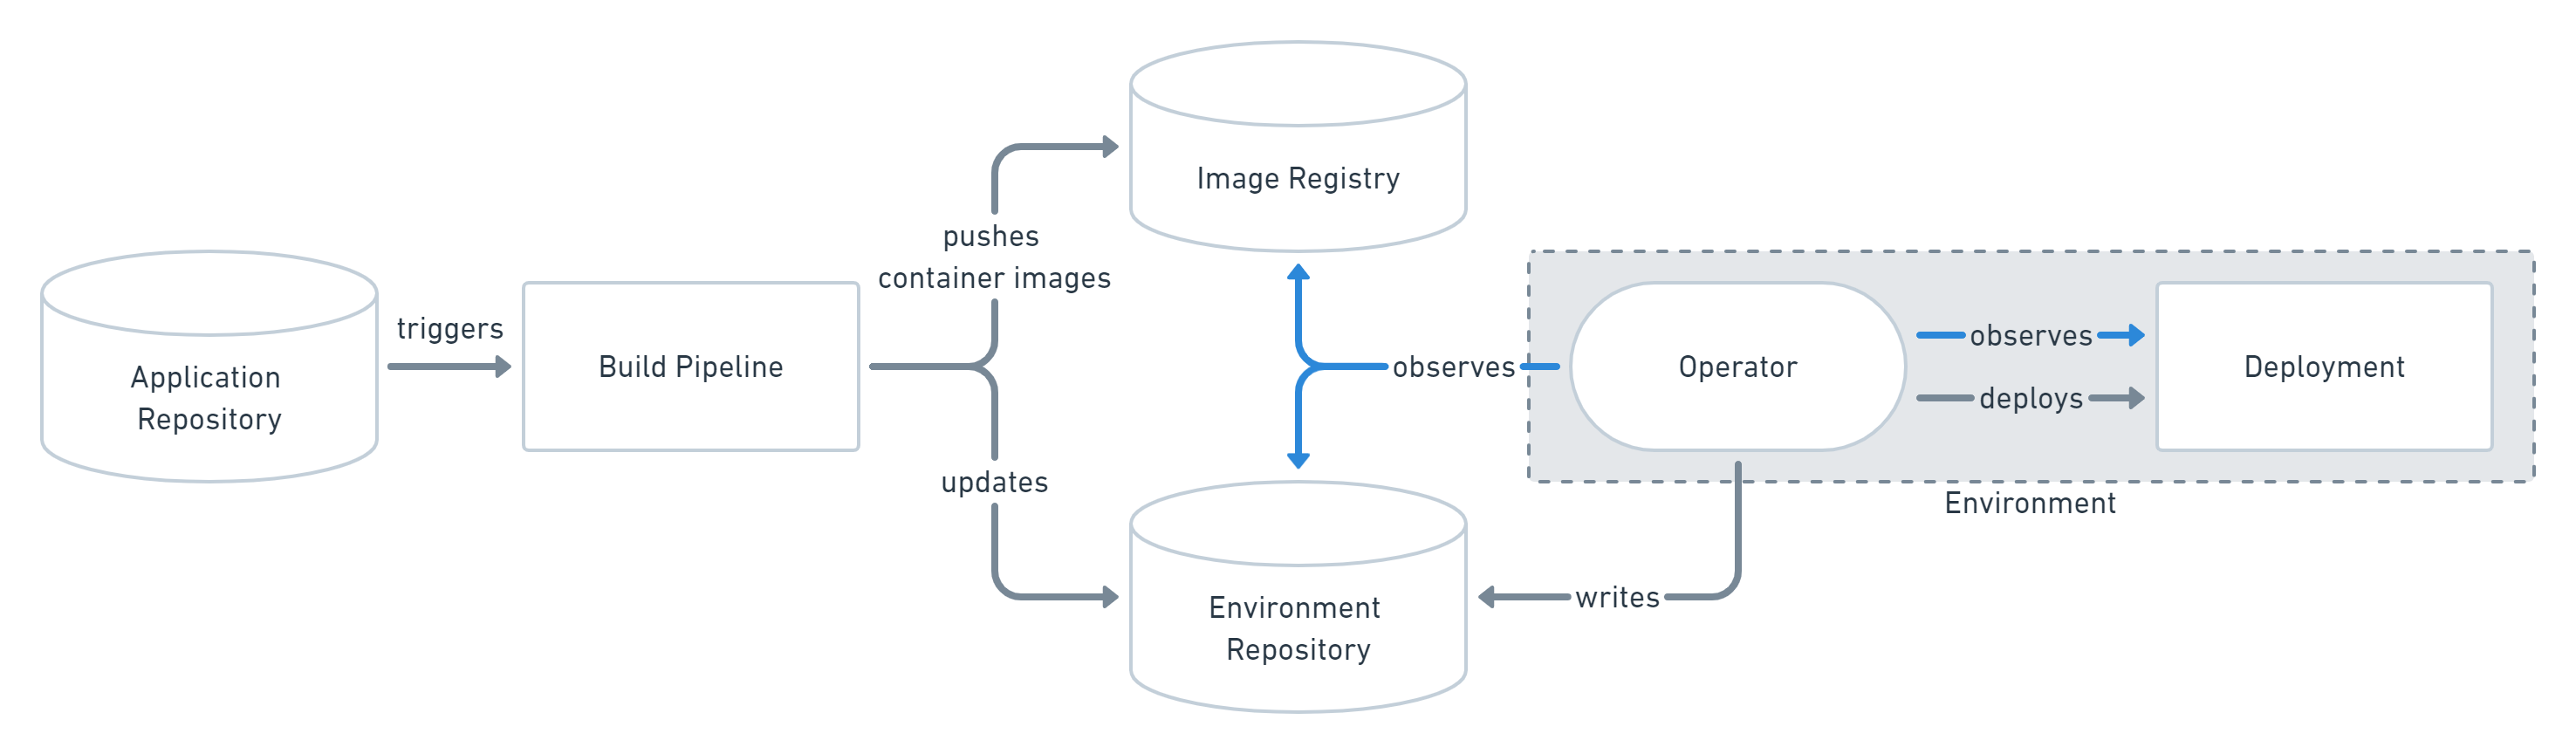
\includegraphics[width=0.9\textwidth]{figures/pull-based-deployments.png}}
  \caption{Flow Pull Based Deployments}
  \label{fig:flow_pull_based_deployments}
\end{figure}

Pada \textbf{Gambar \ref{fig:flow_pull_based_deployments}} mengambarkan flow
pull based deployments yang akan digunakan pada penelitian ini. Pada flow ini
setiap perubahan yang terjadi pada repository akan di-sync dengan kubernetes
cluster melalui ArgoCD sebagai operator yang menjadi observer dan melakukan
sinkronisasi antara status yang diinginkan (yang didefinisikan di Git) dengan
status aktual di cluster.

\section{Implementasi Microservice}\label{sec:bab4_implementasi_microservice}
Implementasi microservice pada penelitian ini terdiri dari beberapa service
yang ditulis menggunakan bahasa pemrograman Go/Golang. Service yang dibuat akan
dilakukan containerization menggunakan Docker agar dapat digunakan sebagai
image pada kubernetes cluster. Setelah containerization selesai, image tersebut
akan dideploy pada kubernetes cluster menggunakan ArgoCD.

Terdapat 4 Service yang akan diimplementasikan yaitu UI Service (Entrypoint),
Auth Service, Color Service, dan Prime Generator Service. UI Service akan
berfungsi sebagai entrypoint untuk user dan akan memanggil service lainnya
berdasarkan permintaan user. Auth Service akan berfungsi sebagai autentikasi
dan otorisasi user sebelum bisa mengakses service lainnya. Color Service akan
berfungsi sebagai service yang akan menghasilkan warna acak berdasarkan
permintaan user. Prime Generator Service akan berfungsi sebagai service yang
akan menghasilkan bilangan prima berdasarkan permintaan user dimana user
menginput batas digit bilangan prima yang diinginkan.

\subsection{Implementasi UI Service}
UI Service atau Frontend service akan menjadi entrypoint dari User agar dapat
mengakses service lainnya. UI Service akan menggunakan bahasa pemrograman
Go/Golang dengan menggunakan HTMX sebagai library untuk pengembangan UI. UI
Service terdiri dari beberapa halaman yaitu halaman login dan halaman dashboard
service yang digunakan untuk menampilkan data dari service lainnya.

\begin{lstlisting}[language=go, 
  basicstyle=\footnotesize\ttfamily,
  caption={Implementasi UI Service Halaman Login},
  label={lst:ui-service-login}]
func serveHome(w http.ResponseWriter, r *http.Request) {
    html := fmt.Sprintf(`<!DOCTYPE html>
<html>
<head>
    <title>HTMX Frontend (Created By Zein)</title>
    <script src="https://unpkg.com/htmx.org@1.9.2"></script>
</head>
<body>
    <h1>Welcome</h1>
    <p><em>Version: %s</em></p>
    <a href="/login">Login to access protected page</a>
</body>
</html>`, version)
    w.Header().Set("Content-Type", "text/html")
    fmt.Fprint(w, html)
}

func serveLogin(w http.ResponseWriter, r *http.Request) {
    html := fmt.Sprintf(`<!DOCTYPE html>
<html>
<head>
    <title>Login</title>
    <script src="https://unpkg.com/htmx.org@1.9.2"></script>
</head>
<body>
    <h2>Login</h2>
    <p><em>Version: %s</em></p>
    <form hx-post="/do_login" hx-target="#login_result" hx-swap="innerHTML">
        <input type="text" name="username" placeholder="Username" required><br>
        <input type="password" name="password" placeholder="Password" required><br>
        <button type="submit">Login</button>
    </form>
    <div id="login_result"></div>
</body>
</html>`, version)
    w.Header().Set("Content-Type", "text/html")
    fmt.Fprint(w, html)
}
\end{lstlisting}
Pada \textbf{Kode Program \ref{lst:ui-service-login}} menampilkan bagian code
untuk halaman login UI Service. Halaman ini akan tampil juga menjadi halama
home UI Service. Pada Gambarxxx menampilkan halaman home sekaligus login page
pada UI Service dimana user dapat login menggunakan username dan password yang
telah diatur pada service Auth Service.
% TODO: Masukan gambar UI service login lalu jelaskan

\begin{lstlisting}[language=go, 
  basicstyle=\footnotesize\ttfamily,
  caption={Implementasi Algoritma Login UI Service},
  label={lst:ui-service-login-handler}]
func handleLogin(w http.ResponseWriter, r *http.Request) {
  username := r.FormValue("username")
  password := r.FormValue("password")

  req, err := http.NewRequest("POST", authServiceURL, nil)
  if err != nil {
      http.Error(w, "Internal error", http.StatusInternalServerError)
      return
  }
  req.SetBasicAuth(username, password)
  resp, err := http.DefaultClient.Do(req)
  if err != nil || resp.StatusCode != http.StatusOK {
      fmt.Fprint(w, "<span style='color:red'>Login failed</span>")
      return
  }

  http.SetCookie(w, &http.Cookie{
      Name:  "session_user",
      Value: username,
      Path:  "/",
  })
  fmt.Fprintf(w, `<span style="color:green">Login successful! <a href="/protected">Go to protected page</a></span><br><em>Version: %s</em>`, version)
}
\end{lstlisting}
Pada \textbf{Kode Program \ref{lst:ui-service-login-handler}} menampilkan
bagian code untuk algoritma login UI Service. Algoritma ini akan melakukan
autentikasi user menggunakan username dan password yang diinputkan oleh user
dan akan mengirimkan request ke service Auth Service untuk memverifikasi
autentikasi user.

\begin{lstlisting}[language=go, 
  basicstyle=\footnotesize\ttfamily,
  caption={Implementasi Dashboard Service},
  label={lst:dashboard-service}]
func serveProtected(w http.ResponseWriter, r *http.Request) {
  cookie, err := r.Cookie("session_user")
  if err != nil || cookie.Value == "" {
    http.Redirect(w, r, "/login", http.StatusFound)
    return
  }

  html := fmt.Sprintf(`<!DOCTYPE html>
<html>
<head>
    <title>Protected Page</title>
    <script src="https://unpkg.com/htmx.org@1.9.2"></script>
</head>
<body>
    <h2>Protected Page</h2>
    <p><em>Version: %s</em></p>
    <p>Welcome, %s!</p>
    <button hx-get="/get_color" hx-target="#color_result" hx-swap="innerHTML">Get Random Color</button>
    <div id="color_result"></div>
    <br>
    <a href="/">Back to Home</a>
</body>
</html>`, version, cookie.Value)
  w.Header().Set("Content-Type", "text/html")
  fmt.Fprint(w, html)
}

func handleGetColor(w http.ResponseWriter, r *http.Request) {
  resp, err := http.Get(colorServiceURL)
  if err != nil {
    http.Error(w, "Failed to get color", http.StatusInternalServerError)
    return
  }
  defer resp.Body.Close()
  color, _ := io.ReadAll(resp.Body)
  fmt.Fprintf(w, "<div style='color:%s'>Random Color: %s<br><em>Version: %s</em></div>", color, color, version)
}
\end{lstlisting}

Pada \textbf{Kode Program \ref{lst:dashboard-service}} menampilkan implementasi
halaman dashboard yang dilindungi (protected page) beserta fungsionalitas untuk
mendapatkan warna acak dari Color Service. Halaman ini hanya dapat diakses oleh
pengguna yang sudah login, yang ditandai dengan adanya session cookie. Fungsi
\texttt{serveProtected} akan mengecek keberadaan cookie session dan menampilkan
halaman dashboard jika valid, sementara \texttt{handleGetColor} akan memanggil
Color Service untuk mendapatkan warna acak yang akan ditampilkan ke pengguna.
cookie session dan menampilkan halaman dashboard jika valid, sementara
\texttt{handleGetColor} akan memanggil Color Service untuk mendapatkan warna
acak yang akan ditampilkan ke pengguna.

\subsection{Implementasi Auth Service}
Auth service sendiri mempunyai fungsionalitas untuk melakukan autentikasi user
agar dapat mengakses dashboard dari UI Service. Auth service akan memvalidasi
username dan password yang diinputkan oleh user dan akan mengirimkan response
ke UI Service untuk menampilkan halaman dashboard.

\begin{lstlisting}[language=go, 
  basicstyle=\footnotesize\ttfamily, 
  caption={Implementasi Auth Service}, 
  label={lst:implementasi-auth-service}]
func main() {
    http.HandleFunc("/auth", func(w http.ResponseWriter, r *http.Request) {
        auth := r.Header.Get("Authorization")
        if !strings.HasPrefix(auth, "Basic ") {
            http.Error(w, "Unauthorized", http.StatusUnauthorized)
            return
        }
        payload, _ := base64.StdEncoding.DecodeString(
          strings.TrimPrefix(auth, "Basic ")
        )
        pair := strings.SplitN(string(payload), ":", 2)
        if len(pair) != 2 || pair[0] != validUser || pair[1] != validPass {
            http.Error(w, "Unauthorized", http.StatusUnauthorized)
            return
        }
        w.WriteHeader(http.StatusOK)
        w.Write([]byte("OK"))
    })
    http.ListenAndServe(":8080", nil)
}
\end{lstlisting}

Pada \textbf{Kode Program \ref{lst:implementasi-auth-service}} menampilkan
bagian code untuk algoritma autentikasi user. Algoritma ini akan melakukan
autentikasi user menggunakan username dan password yang diinputkan oleh user
dan akan mengirimkan response ke UI Service untuk menampilkan halaman
dashboard.

\subsection{Implementasi Color Service}
Color service sendiri mempunyai fungsionalitas untuk mendapatkan warna acak
yang akan ditampilkan ke pengguna. Pada \textbf{Kode Program
  \ref{lst:color-service}} menampilkan bagian code untuk algoritma color service.
Algoritma ini akan mendapatkan warna acak yang akan menjadi response dari Color
Service. Color Service akan mengirimkan response tersebut ke UI Service yang
akan menampilkan warna acak tersebut ke pengguna.

\begin{lstlisting}[language=go, 
  basicstyle=\footnotesize\ttfamily,
  caption={Implementasi Color Service},
  label={lst:color-service}]
func main() {
  http.HandleFunc("/get_color", func(w http.ResponseWriter, r *http.Request) {
      colors := []string{"red", "green", "blue", "yellow", "purple", "orange"}
      color := colors[rand.Intn(len(colors))]
      fmt.Fprint(w, color)
  })
  http.ListenAndServe(":8080", nil)
}
\end{lstlisting}

\subsection{Implementasi Prime Generator Service}
Prime generator service sendiri mempunyai fungsionalitas untuk mendapatkan
bilangan prima berdasarkan input dari user. User akan melalukan input berupa
jumlah digit bilangan prima yang diinginkan dan akan mendapatkan response
berupa bilangan prima yang diinginkan. Pada \textbf{Table
  \ref{tab:implementasi-prime-generator-service}} menampilkan bagian code untuk
algoritma prime generator service. Algoritma ini akan mendapatkan bilangan
prima berdasarkan input dari user dan akan mengirimkan response tersebut ke UI
Service yang akan menampilkan bilangan prima tersebut ke pengguna.

\begin{table}[H]
  \centering
  \begin{minipage}{0.95\linewidth}
    \begin{lstlisting}[language=go, basicstyle=\footnotesize\ttfamily]
func generatePrimes(digit int) ([]int, error) {
  if digit < 1 || digit > 6 {
    return nil, fmt.Errorf("digit must be between 1 and 6")
  }
  min := 1
  for i := 1; i < digit; i++ {
    min *= 10
  }
  max := min*10 - 1

  primes := []int{}
  rand.Seed(time.Now().UnixNano())
  attempts := 0
  for len(primes) < 3 && attempts < 10000 {
    num := rand.Intn(max-min+1) + min
    if isPrime(num) {
      already := false
      for _, p := range primes {
        if p == num {
          already = true
          break
        }
      }
      if !already {
        primes = append(primes, num)
      }
    }
    attempts++
  }
  if len(primes) < 3 {
    return nil, fmt.Errorf("could not find 3 prime numbers with %d digits", digit)
  }
  return primes, nil
}
    \end{lstlisting}
  \end{minipage}
  \caption{Implementasi Prime Generator Service}
  \label{tab:implementasi-prime-generator-service}
\end{table}

\section{Testing}
Setelah menyelesaikan tahap implementasi pada bagian
\textbf{\ref{sec:bab4_instalasi_infrastruktur_mesin} Instalasi Infrastruktur
  Mesin} serta \textbf{\ref{sec:bab4_implementasi_argocd} Instalasi ArgoCD}, dan
juga \textbf{\ref{sec:bab4_implementasi_microservice} Implementasi
  Microservice}. Selanjutnya perlu dilakukan pengujian untuk memastikan seluruh
komponen berfungsi seperti yang diharapkan. Pengujian ini mencakup beberapa
aspek penting termasuk fungsionalitas Kubernetes cluster, integrasi ArgoCD,
fungsionalitas microservice, serta alur kerja GitOps yang telah diterapkan.
Melalui pengujian menyeluruh ini, diharapkan dapat dievaluasi sejauh mana
solusi yang dibangun mampu memenuhi kebutuhan pengembangan dan operasional
aplikasi secara efisien.

Pengujian yang dilakukan pada tahap ini adalah pengujian black-box testing pada
flow automatic deployment, serta komponen ArgoCD. Testing akan dilakukan secara
manual mengikuti flow pull based deployments dimana testing ini dikategorikan
sebagai Black-box testing dikarenakan tidak ada perubahan pada kode ArgoCD.
Untuk pengujian pada microservice nya sendiri dilakukan unit testing yang
dilakukan pada internal khusus nya algoritma yang ada pada microservice
tersebut.

\subsection{Pengujian (Testing) Pada Microservice}\label{subsec:bab4_pengujian_microservice}
Pengujian testing yang dilakukan terhadap sistem microservice pada tahap ini
menggunakan metode unit testing dan fungsional testing secara keseluruhan
melalui UI. Terdapat 4 Service yang akan diuji pada tahap ini yaitu Auth
Service, Color Service, Prime Generator Service, dan UI Service. Khusus untuk
UI Service sendiri hanya akan dilakukan fungsional testing berupa validasi UI.
\begin{table}[H]
  \centering
  \small
  \begin{adjustbox}{width=\textwidth}
    \begin{tabular}{|p{0.8cm}|p{2.6cm}|p{4.5cm}|p{3.8cm}|p{1.2cm}|}
      \hline
      \textbf{Kode Uji}                                                           & \textbf{Nama Uji}                  & \textbf{Kasus Uji} & \textbf{Hasil Yang Diharapkan} & \textbf{Status} \\
      \hline
      FT-001                                                                      & Akses Halaman Utama                &
      \begin{enumerate}[leftmargin=*,noitemsep,topsep=0pt,label=\arabic*.,widest=99]
        \item Buka \texttt{/}
      \end{enumerate}             &
      Halaman selamat datang tampil dengan info versi dan link login              & Valid                                                                                                      \\ \hline

      FT-002                                                                      & Akses Halaman Login                &
      \begin{enumerate}[leftmargin=*,noitemsep,topsep=0pt,label=\arabic*.,widest=99]
        \item Buka \texttt{/login}
      \end{enumerate}            &
      Form login dengan field username, password, dan info versi tampil           & Valid                                                                                                      \\ \hline

      FT-003                                                                      & Login Berhasil                     &
      \begin{enumerate}[leftmargin=*,noitemsep,topsep=0pt,label=\arabic*.,widest=99]
        \item Masukkan username dan password valid
        \item Submit form login
      \end{enumerate}            &
      Cookie session tersimpan, muncul pesan sukses dan link ke halaman protected & Valid                                                                                                      \\ \hline

      FT-004                                                                      & Login Gagal                        &
      \begin{enumerate}[leftmargin=*,noitemsep,topsep=0pt,label=\arabic*.,widest=99]
        \item Masukkan username atau password tidak valid
        \item Submit form login
      \end{enumerate}            &
      Muncul pesan "Login failed" berwarna merah                                  & Valid                                                                                                      \\ \hline

      FT-005                                                                      & Akses Protected (Belum Login)      &
      \begin{enumerate}[leftmargin=*,noitemsep,topsep=0pt,label=\arabic*.,widest=99]
        \item Akses \texttt{/protected} tanpa cookie session
      \end{enumerate}            &
      Dialihkan ke halaman login                                                  & Valid                                                                                                      \\ \hline

      FT-006                                                                      & Akses Protected (Sudah Login)      &
      \begin{enumerate}[leftmargin=*,noitemsep,topsep=0pt,label=\arabic*.,widest=99]
        \item Login dengan kredensial valid
        \item Akses \texttt{/protected}
      \end{enumerate}            &
      Tampil pesan selamat datang, tombol warna, dan form generate prime          & Valid                                                                                                      \\ \hline

      FT-007                                                                      & Generate Warna Acak                &
      \begin{enumerate}[leftmargin=*,noitemsep,topsep=0pt,label=\arabic*.,widest=99]
        \item Klik tombol "Get Random Color" pada halaman protected
      \end{enumerate}            &
      Nama warna acak tampil sesuai warna dan info versi                          & Valid                                                                                                      \\ \hline

      FT-008                                                                      & Generate Prime (Input Valid)       &
      \begin{enumerate}[leftmargin=*,noitemsep,topsep=0pt,label=\arabic*.,widest=99]
        \item Isi digit antara 1-6 pada form generate prime
        \item Submit form
      \end{enumerate}            &
      Bilangan prima tampil dengan info versi                                     & Valid                                                                                                      \\ \hline

      FT-009                                                                      & Generate Prime (Input Tidak Valid) &
      \begin{enumerate}[leftmargin=*,noitemsep,topsep=0pt,label=\arabic*.,widest=99]
        \item Isi digit kurang dari 1 atau lebih dari 6 pada form generate prime
        \item Submit form
      \end{enumerate}    &
      Muncul pesan error berwarna merah                                           & Valid                                                                                                      \\ \hline

    \end{tabular}
  \end{adjustbox}
  \caption{Daftar Test Case Fungsional Frontend Service}
  \label{tab:test-case-frontend}
\end{table}

Pada \textbf{Table \ref{tab:test-case-frontend}} dapat dilihat daftar test case
yang telah dilakukan beserta hasilnya. Test tersebut dilakukan secara manual
dengan pendekatan black-box testing. Setiap test case dirancang untuk
memverifikasi fitur-fitur kunci dari Frontend Service dalam mendukung alur
kerja aplikasi.

% Test case auth service
Berikut adalah table kasus test yang dilakukan uji pada kode Auth Service dan
kode unit test Auth Service.
\begin{table}[H]
  \centering
  \small
  \begin{adjustbox}{width=\textwidth}
    \begin{tabular}{|p{1.5cm}|p{3.2cm}|p{5cm}|p{3.2cm}|p{1.2cm}|}
      \hline
      \textbf{Kode Uji}                                                                & \textbf{Nama Uji}          & \textbf{Kasus Uji} & \textbf{Hasil Yang Diharapkan} & \textbf{Status} \\
      \hline
      TC-AUTH-001                                                                      & Kredensial Valid           &
      \begin{enumerate}[leftmargin=*,noitemsep,topsep=0pt,label=\arabic*.,widest=99]
        \item Kirim request dengan \texttt{Authorization: Basic dXNlcjpwYXNz}
      \end{enumerate}            &
      HTTP 200 OK dengan respons "OK"                                                  & Valid                                                                                              \\ \hline

      TC-AUTH-002                                                                      & Kredensial Tidak Valid     &
      \begin{enumerate}[leftmargin=*,noitemsep,topsep=0pt,label=\arabic*.,widest=99]
        \item Kirim request dengan \texttt{Authorization: Basic d3Jvbmc6cGFzcw==}
      \end{enumerate}        &
      HTTP 401 Unauthorized                                                            & Valid                                                                                              \\ \hline

      TC-AUTH-003                                                                      & Tanpa Header Authorization &
      \begin{enumerate}[leftmargin=*,noitemsep,topsep=0pt,label=\arabic*.,widest=99]
        \item Kirim request tanpa header Authorization
      \end{enumerate}                 &
      HTTP 401 Unauthorized                                                            & Valid                                                                                              \\ \hline

      TC-AUTH-004                                                                      & Header Tidak Sesuai Format &
      \begin{enumerate}[leftmargin=*,noitemsep,topsep=0pt,label=\arabic*.,widest=99]
        \item Kirim request dengan \texttt{Authorization: Bearer token}
      \end{enumerate}                 &
      HTTP 401 Unauthorized                                                            & Valid                                                                                              \\ \hline

      TC-AUTH-005                                                                      & Base64 Tidak Valid         &
      \begin{enumerate}[leftmargin=*,noitemsep,topsep=0pt,label=\arabic*.,widest=99]
        \item Kirim request dengan \texttt{Authorization: Basic invalid\_base64\_string}
      \end{enumerate} &
      HTTP 401 Unauthorized                                                            & Valid                                                                                              \\ \hline

      TC-AUTH-006                                                                      & Tanpa Password             &
      \begin{enumerate}[leftmargin=*,noitemsep,topsep=0pt,label=\arabic*.,widest=99]
        \item Kirim request dengan \texttt{Authorization: Basic dXNlcg==}
      \end{enumerate}                &
      HTTP 401 Unauthorized                                                            & Valid                                                                                              \\ \hline

      TC-AUTH-007                                                                      & Kredensial Kosong          &
      \begin{enumerate}[leftmargin=*,noitemsep,topsep=0pt,label=\arabic*.,widest=99]
        \item Kirim request dengan \texttt{Authorization: Basic}
      \end{enumerate}                 &
      HTTP 401 Unauthorized                                                            & Valid                                                                                              \\ \hline
    \end{tabular}
  \end{adjustbox}
  \caption{Daftar Kasus Uji Fungsional Layanan Autentikasi}
  \label{tab:auth-test-cases}
\end{table}
\begin{lstlisting}[language=go, 
  basicstyle=\footnotesize\ttfamily,
  caption={Kode Unit Testing Pada Auth Service},
  label={lst:unit-test-auth-service}
]
func TestAuthHandler(t *testing.T) {
  tests := []struct {
      name           string
      authHeader     string
      expectedStatus int
      expectedBody   string
  }{
      {"Valid Credentials", "Basic " + base64.StdEncoding.EncodeToString([]byte("user:pass")), http.StatusOK, "OK"},
      {"Invalid Credentials", "Basic " + base64.StdEncoding.EncodeToString([]byte("wrong:pass")), http.StatusUnauthorized, "Unauthorized\n"},
      {"Missing Header", "", http.StatusUnauthorized, "Unauthorized\n"},
      {"Malformed Header", "Bearer token", http.StatusUnauthorized, "Unauthorized\n"},
      {"Invalid Base64", "Basic invalid_base64", http.StatusUnauthorized, "Unauthorized\n"},
      {"Missing Password", "Basic " + base64.StdEncoding.EncodeToString([]byte("user")), http.StatusUnauthorized, "Unauthorized\n"},
      {"Empty Credentials", "Basic ", http.StatusUnauthorized, "Unauthorized\n"},
  }

  for _, tt := range tests {
      t.Run(tt.name, func(t *testing.T) {
          log.Printf("[START] Test case: %s", tt.name)

          req, err := http.NewRequest("GET", "/auth", nil)
          if err != nil {
              t.Fatal(err)
          }

          if tt.authHeader != "" {
              req.Header.Set("Authorization", tt.authHeader)
          }

          rr := httptest.NewRecorder()
          handler := http.HandlerFunc(authHandler)
          handler.ServeHTTP(rr, req)

          status := rr.Code
          body := rr.Body.String()

          if status != tt.expectedStatus {
              t.Errorf("[FAIL] %s: expected status %d, got %d", tt.name, tt.expectedStatus, status)
          } else {
              log.Printf("[PASS] %s: status %d as expected", tt.name, status)
          }

          if body != tt.expectedBody {
              t.Errorf("[FAIL] %s: expected body %q, got %q", tt.name, tt.expectedBody, body)
          } else {
              log.Printf("[PASS] %s: body %q as expected", tt.name, body)
          }

          log.Printf("[END] Test case: %s\n", tt.name)
      })
  }
}
Output:
=== RUN   TestAuthHandler
--- PASS: TestAuthHandler (0.00s)
    --- PASS: TestAuthHandler/Valid_Credentials (0.00s)
    --- PASS: TestAuthHandler/Invalid_Credentials (0.00s)
    --- PASS: TestAuthHandler/Missing_Header (0.00s)
    --- PASS: TestAuthHandler/Malformed_Header (0.00s)
    --- PASS: TestAuthHandler/Invalid_Base64 (0.00s)
    --- PASS: TestAuthHandler/Missing_Password (0.00s)
    --- PASS: TestAuthHandler/Empty_Credentials (0.00s)
PASS
ok      auth-service    0.007s
\end{lstlisting}

Pada \textbf{Table \ref{tab:auth-test-cases}} adalah pengujian yang dilakukan
pada code Auth Service. Test tersebut dilakukan menggunakan unit test dengan
pendekatan validasi fungsionalitas terhadap code Auth Service. Pada
\textbf{Kode Program \ref{lst:unit-test-auth-service}} adalah penerapan pada
code unit testing pada Auth Service.

% Test case Prime Generator
Berikut ini adalah unit test yang dilakukan uji pada kode Prime Generator
Service.
\begin{table}[H]
  \centering
  \small
  \begin{adjustbox}{width=\textwidth}
    \begin{tabular}{|p{0.8cm}|p{2.6cm}|p{4.5cm}|p{3.8cm}|p{1.2cm}|}
      \hline
      \textbf{Kode Uji}                                                             & \textbf{Nama Uji}                  & \textbf{Kasus Uji} & \textbf{Hasil Yang Diharapkan} & \textbf{Status} \\
      \hline
      UT-001                                                                        & Generate Prime (Digit Valid)       &
      \begin{enumerate}[leftmargin=*,noitemsep,topsep=0pt,label=\arabic*.,widest=99]
        \item Kirim POST ke \texttt{/generate\_prime} dengan digit 1, 2, atau 6
      \end{enumerate}       &
      Status 200 OK, respons berisi 3 bilangan prima unik dengan digit sesuai input & Valid                                                                                                      \\ \hline

      UT-002                                                                        & Generate Prime (Digit Tidak Valid) &
      \begin{enumerate}[leftmargin=*,noitemsep,topsep=0pt,label=\arabic*.,widest=99]
        \item Kirim POST ke \texttt{/generate\_prime} dengan digit 0, 7, atau negatif
      \end{enumerate} &
      Status 400 Bad Request, respons berisi pesan error                            & Valid                                                                                                      \\ \hline

      UT-003                                                                        & Method Not Allowed                 &
      \begin{enumerate}[leftmargin=*,noitemsep,topsep=0pt,label=\arabic*.,widest=99]
        \item Kirim GET ke \texttt{/generate\_prime}
      \end{enumerate}              &
      Status 405 Method Not Allowed, respons berisi pesan error                     & Valid                                                                                                      \\ \hline

      UT-004                                                                        & Invalid JSON Payload               &
      \begin{enumerate}[leftmargin=*,noitemsep,topsep=0pt,label=\arabic*.,widest=99]
        \item Kirim POST ke \texttt{/generate\_prime} dengan body bukan JSON
      \end{enumerate}          &
      Status 400 Bad Request, respons berisi pesan error                            & Valid                                                                                                      \\ \hline

    \end{tabular}
  \end{adjustbox}
  \caption{Daftar Unit Test Case Prime Generator Service}
  \label{tab:unit-test-prime-generator}
\end{table}
\begin{lstlisting}[language=go, 
  basicstyle=\footnotesize\ttfamily, 
  caption={Kode Unit Testing Pada Prime Generator Service}, 
  label={lst:unit-test-prime-generator}]
func TestGeneratePrimes(t *testing.T) {
  tests := []struct {
    digit       int
    expectsErr  bool
    description string
  }{
    {1, false, "Valid digit 1"},
    {2, false, "Valid digit 2"},
    {6, false, "Valid digit 6"},
    {0, true, "Invalid digit 0"},
    {7, true, "Invalid digit 7"},
    {-1, true, "Negative digit"},
  }

  for _, tt := range tests {
    reqBody, _ := json.Marshal(requestPayload{Digit: tt.digit})
    req := httptest.NewRequest(http.MethodPost, "/generate_prime", bytes.NewReader(reqBody))
    w := httptest.NewRecorder()

    generatePrimeHandler(w, req)

    resp := w.Result()
    var respPayload responsePayload
    json.NewDecoder(resp.Body).Decode(&respPayload)

    if tt.expectsErr {
      if resp.StatusCode == http.StatusOK {
        t.Errorf("%s: expected error but got success", tt.description)
      }
      if respPayload.Error == "" {
        t.Errorf("%s: expected error message but got none", tt.description)
      }
    } else {
      if resp.StatusCode != http.StatusOK {
        t.Errorf("%s: expected success but got status %d", tt.description, resp.StatusCode)
      } else {
        log.Printf("%s: success with primes %v", tt.description, respPayload.Primes)
      }
      if len(respPayload.Primes) != 3 {
        t.Errorf("%s: expected 3 primes but got %d", tt.description, len(respPayload.Primes))
      }
    }
  }
}
Output: 
=== RUN   TestGeneratePrimes
2025/06/27 20:05:38 Valid digit 1: success with primes [3 5 7]
2025/06/27 20:05:38 Valid digit 2: success with primes [97 31 89]
2025/06/27 20:05:38 Valid digit 6: success with primes [143609 463613 117371]
--- PASS: TestGeneratePrimes (0.00s)
PASS
ok      prime-service   0.006s
\end{lstlisting}
\begin{lstlisting}[language=go, 
  basicstyle=\footnotesize\ttfamily,
  caption={Kode Unit Testing Pada Prime Generator Service 2},
  label={lst:unit-test-prime-generator-output}
]
func TestGeneratePrimeHandler_MethodNotAllowed(t *testing.T) {
  req := httptest.NewRequest(http.MethodGet, "/generate_prime", nil)
  w := httptest.NewRecorder()

  generatePrimeHandler(w, req)

  resp := w.Result()
  if resp.StatusCode != http.StatusMethodNotAllowed {
    t.Errorf("Expected status 405 Method Not Allowed but got %d", resp.StatusCode)
  } else {
    log.Printf("MethodNotAllowed test: success with status %d", resp.StatusCode)
  }
}
Output:
=== RUN   TestGeneratePrimeHandler_MethodNotAllowed
2025/06/28 15:11:02 MethodNotAllowed test: success with status 405
--- PASS: TestGeneratePrimeHandler_MethodNotAllowed (0.00s)
PASS
ok      prime-service   0.007s
\end{lstlisting}

Pada \textbf{Table \ref{tab:unit-test-prime-generator}} adalah pengujian yang
dilakukan pada code Prime Generator Service. Test tersebut dilakukan
menggunakan unit testing dengan pendekatan validasi fungsionalitas terhadap
response yang diharapkan. Setiap test case dirancang untuk memverifikasi
fitur-fitur kunci dari Prime Generator Service dalam mendukung alur kerja
aplikasi. Penerapan code unit testing dan output pada setiap testin tersebut
dapat dilihat pada \textbf{Kode Program \ref{lst:unit-test-prime-generator}}
dan \textbf{Kode Program \ref{lst:unit-test-prime-generator-output}}.

% Test Case Color Service
Pengujian yang dilakukan pada Color Service menggunakan unit testing dengan
pendekatan validasi fungsionalitas terhadap response yang diharapkan. Setiap
test case dirancang untuk memverifikasi fitur-fitur kunci dari Color Service
dalam mendukung alur kerja aplikasi.
\begin{table}[H]
  \centering
  \small
  \begin{adjustbox}{width=\textwidth}
    \begin{tabular}{|p{1.5cm}|p{3.2cm}|p{5cm}|p{3.2cm}|p{1.2cm}|}
      \hline
      \textbf{Kode Uji}                                                                                                                                                               & \textbf{Nama Uji}         & \textbf{Kasus Uji} & \textbf{Hasil Yang Diharapkan} & \textbf{Status} \\
      \hline
      TC-COLOR-001                                                                                                                                                                    & Get Random Color (Normal) &
      \begin{enumerate}[leftmargin=*,noitemsep,topsep=0pt,label=\arabic*.,widest=99]
        \item Kirim request GET ke endpoint \texttt{/color}
      \end{enumerate}                                                                                                                &
      HTTP 200 OK, respons berupa salah satu warna: \texttt{red}, \texttt{green}, \texttt{blue}, \texttt{yellow}, \texttt{purple}, \texttt{orange}, \texttt{pink}, atau \texttt{cyan} & Valid                                                                                             \\ \hline

      TC-COLOR-002                                                                                                                                                                    & Method Not Allowed        &
      \begin{enumerate}[leftmargin=*,noitemsep,topsep=0pt,label=\arabic*.,widest=99]
        \item Kirim request POST ke endpoint \texttt{/color}
      \end{enumerate}                                                                                                                &
      HTTP 405 Method Not Allowed                                                                                                                                                     & Valid                                                                                             \\ \hline

      TC-COLOR-003                                                                                                                                                                    & Endpoint Not Found        &
      \begin{enumerate}[leftmargin=*,noitemsep,topsep=0pt,label=\arabic*.,widest=99]
        \item Kirim request GET ke endpoint yang tidak ada, misal \texttt{/wrong}
      \end{enumerate}                                                                                                       &
      HTTP 404 Not Found                                                                                                                                                              & Valid                                                                                             \\ \hline
    \end{tabular}
  \end{adjustbox}
  \caption{Daftar Kasus Uji Fungsional Layanan Color}
  \label{tab:color-test-cases}
\end{table}

Pada \textbf{Table \ref{tab:color-test-cases}} adalah pengujian yang dilakukan
pada code Color Service. Test tersebut dilakukan menggunakan unit testing
dengan pendekatan validasi fungsionalitas terhadap response yang diharapkan.
Setiap test case dirancang untuk memverifikasi fitur-fitur kunci dari Color
Service dalam mendukung alur kerja aplikasi. Penerapan code unit testing dan
output pada setiap testing tersebut dapat dilihat pada \textbf{Kode Program
  \ref{lst:unit-test-color-service}}.

\begin{lstlisting}[language=go, 
  basicstyle=\footnotesize\ttfamily, 
  caption={Kode Unit Testing Pada Color Service}, 
  label={lst:unit-test-color-service}
]
func TestColorHandler(t *testing.T) {
  t.Run("GET /color returns valid color", func(t *testing.T) {
    req := httptest.NewRequest("GET", "/color", nil)
    w := httptest.NewRecorder()
    colorHandler(w, req)

    resp := w.Result()
    defer resp.Body.Close()

    if resp.StatusCode != http.StatusOK {
      t.Errorf("Expected status 200, got %d", resp.StatusCode)
    }

    validColors := map[string]bool{
      "red": true, "green": true, "blue": true, "yellow": true,
      "purple": true, "orange": true, "pink": true, "cyan": true,
    }

    buf := make([]byte, 16)
    n, _ := resp.Body.Read(buf)
    color := strings.TrimSpace(string(buf[:n]))

    if !validColors[color] {
      t.Errorf("Unexpected color returned: %q", color)
    }
  })

  t.Run("POST /color returns 405", func(t *testing.T) {
    req := httptest.NewRequest("POST", "/color", nil)
    w := httptest.NewRecorder()
    colorHandler(w, req)

    resp := w.Result()
    defer resp.Body.Close()

    if resp.StatusCode != http.StatusMethodNotAllowed {
      t.Errorf("Expected status 405, got %d", resp.StatusCode)
    }
  })

  t.Run("GET /wrong returns 404", func(t *testing.T) {
    req := httptest.NewRequest("GET", "/wrong", nil)
    w := httptest.NewRecorder()

    http.NotFoundHandler().ServeHTTP(w, req)

    resp := w.Result()
    defer resp.Body.Close()

    if resp.StatusCode != http.StatusNotFound {
      t.Errorf("Expected status 404, got %d", resp.StatusCode)
    }
  })
}
Output:
=== RUN   TestColorHandler
=== RUN   TestColorHandler/GET_/color_returns_valid_color
=== RUN   TestColorHandler/POST_/color_returns_405
=== RUN   TestColorHandler/GET_/wrong_returns_404
--- PASS: TestColorHandler (0.00s)
    --- PASS: TestColorHandler/GET_/color_returns_valid_color (0.00s)
    --- PASS: TestColorHandler/POST_/color_returns_405 (0.00s)
    --- PASS: TestColorHandler/GET_/wrong_returns_404 (0.00s)
PASS
ok      color-service   0.007s
\end{lstlisting}

\subsection{Pengujian (Testing) Pada ArgoCD}\label{sec:bab4_pengujian}
Pengujian testing yang dilakukan terhadap sistem ArgoCD pada tahap ini
menggunakan metode validasi (validation). Metode validasi yang digunakan dalam
melakukan pengujian ini berfungsi untuk mengetahui valid atau tidaknya sebuah
fungsi dari sistem yang dibangun. Melakukan pengujian black-box dengan metode
validasi ini juga menentukan apakah sistem telah sesuai seperti apa yang
diinginkan oleh stakeholder pada tahap perencanaan. Pengujian black-box ini
dilakukan dengan jumlah test case sebanyak 15 (lima belas) yang mencakup
berbagai aspek fungsionalitas ArgoCD.

Pengujian dilakukan dengan pendekatan black-box testing yang berfokus pada
fungsionalitas sistem tanpa memperhatikan struktur internal kode. Setiap test
case dirancang untuk memverifikasi fitur-fitur kunci dari ArgoCD dalam
mendukung alur kerja GitOps.Berikut adalah daftar test case yang telah
dilakukan beserta hasilnya:
\begin{table}[h]
  \centering
  \small
  \begin{adjustbox}{width=\textwidth}
    \begin{tabular}{|p{0.8cm}|p{2.2cm}|p{4cm}|p{3.5cm}|p{1.2cm}|}
      \hline
      \textbf{Kode Uji} & \textbf{Nama Uji}         & \textbf{Kasus Uji}                                                & \textbf{Hasil Yang Diharapkan}                                     & \textbf{Status} \\
      \hline
      BT-001            & Login ke Dashboard ArgoCD & \begin{enumerate}[leftmargin=*,noitemsep,topsep=0pt,label=\arabic*.,widest=99]
                                                        \item Buka halaman login ArgoCD
                                                        \item Masukkan kredensial admin
                                                        \item Klik tombol login
                                                      \end{enumerate}  & Pengguna berhasil login dan diarahkan ke dashboard utama           & Valid                                                            \\ \hline
      BT-002            & Tambah Aplikasi Baru      & \begin{enumerate}[leftmargin=*,noitemsep,topsep=0pt,label=\arabic*.,widest=99]
                                                        \item Klik "New App"
                                                        \item Isi form dengan detail aplikasi
                                                        \item Klik "Create"
                                                      \end{enumerate} & Aplikasi baru berhasil dibuat dan muncul di daftar aplikasi        & Valid                                                             \\ \hline
      BT-003            & Sinkronisasi Otomatis     & \begin{enumerate}[leftmargin=*,noitemsep,topsep=0pt,label=\arabic*.,widest=99]
                                                        \item Buat perubahan pada file konfigurasi di repo Git
                                                        \item Push perubahan ke branch yang dimonitor
                                                      \end{enumerate} & ArgoCD mendeteksi perubahan dan melakukan sinkronisasi otomatis    & Valid                                                             \\ \hline
      BT-004            & Rollback Aplikasi         & \begin{enumerate}[leftmargin=*,noitemsep,topsep=0pt,label=\arabic*.,widest=99]
                                                        \item Pilih aplikasi
                                                        \item Klik "History and Rollback"
                                                        \item Pilih versi sebelumnya
                                                        \item Klik "Sync"
                                                      \end{enumerate} & Aplikasi berhasil di-rollback ke versi sebelumnya                  & Valid                                                             \\ \hline
      BT-005            & Validasi Status Kesehatan & \begin{enumerate}[leftmargin=*,noitemsep,topsep=0pt,label=\arabic*.,widest=99]
                                                        \item Deploy aplikasi dengan konfigurasi salah
                                                        \item Periksa status di dashboard
                                                      \end{enumerate} & Menampilkan status "Degraded" atau "Error" dengan pesan yang jelas & Valid                                                             \\ \hline
      BT-006            & Pencarian Aplikasi        & \begin{enumerate}[leftmargin=*,noitemsep,topsep=0pt,label=\arabic*.,widest=99]
                                                        \item Gunakan fitur search di dashboard
                                                        \item Masukkan nama aplikasi
                                                      \end{enumerate} & Menampilkan aplikasi yang sesuai dengan kata kunci pencarian       & Valid                                                             \\ \hline
      BT-007            & Filter Aplikasi           & \begin{enumerate}[leftmargin=*,noitemsep,topsep=0pt,label=\arabic*.,widest=99]
                                                        \item Gunakan filter berdasarkan status/kategori
                                                        \item Pilih filter tertentu
                                                      \end{enumerate} & Menampilkan aplikasi yang sesuai dengan filter yang dipilih        & Valid                                                             \\ \hline
    \end{tabular}
  \end{adjustbox}
  \caption{Daftar Test Case Black-Box Testing}
  \label{tab:test-case}
\end{table}

\newpage
\clearpage
\begin{table}[H]
  \centering
  \small
  \begin{adjustbox}{width=\textwidth}
    \begin{tabular}{|p{0.8cm}|p{2.2cm}|p{4cm}|p{3.5cm}|p{1.2cm}|}
      \hline
      \textbf{Kode Uji} & \textbf{Nama Uji}       & \textbf{Kasus Uji}                                                      & \textbf{Hasil Yang Diharapkan}                               & \textbf{Status} \\
      \hline
      BT-008            & Manajemen Kluster       & \begin{enumerate}[leftmargin=*,noitemsep,topsep=0pt,label=\arabic*.,widest=99]
                                                      \item Tambah kluster baru
                                                      \item Verifikasi koneksi
                                                    \end{enumerate}       & Kluster baru terdaftar dan terhubung dengan status "Healthy" & Valid                                                             \\ \hline
      BT-009            & Logout                  & \begin{enumerate}[leftmargin=*,noitemsep,topsep=0pt,label=\arabic*.,widest=99]
                                                      \item Klik profil pengguna
                                                      \item Pilih "Logout"
                                                    \end{enumerate}       & Pengguna berhasil logout dan diarahkan ke halaman login      & Valid                                                             \\ \hline
      BT-010            & Responsivitas UI        & \begin{enumerate}[leftmargin=*,noitemsep,topsep=0pt,label=\arabic*.,widest=99]
                                                      \item Akses dashboard dari berbagai perangkat (desktop, tablet, mobile)
                                                    \end{enumerate} & Tampilan UI menyesuaikan dengan ukuran layar                 & Valid                                                                   \\ \hline
      BT-011            & Notifikasi Sinkronisasi & \begin{enumerate}[leftmargin=*,noitemsep,topsep=0pt,label=\arabic*.,widest=99]
                                                      \item Lakukan sinkronisasi manual
                                                      \item Periksa notifikasi
                                                    \end{enumerate}       & Muncul notifikasi yang menampilkan status sinkronisasi       & Valid                                                             \\ \hline
    \end{tabular}
  \end{adjustbox}
  \caption{Daftar Test Case Black-Box Testing (Lanjutan)}
  \label{tab:test-case-2}
\end{table}

\subsubsection{Pegujian Flow Automatic Deployment pada ArgoCD}
Pada pengujian ini akan dilakukan pengujian flow automatic deployment pada
service yang telah diimplementasikan pada
\textbf{\ref{sec:bab4_implementasi_microservice} Implementasi Microservice}.
Pengujian tahap ini akan mengikuti flow seperti pada gambar \textbf{Gambar
  \ref{fig:flow_pull_based_deployments}}. Hanya ada satu uji yang akan diuji pada
tahap ini yaitu flow pull based deployment. Validasi dari pengujian yang
dilakukan adalah berdasarkan perubahan yang terjadi pada kode service dan juga
manifest yang terdeploy pada ArgoCD.

\subsection{Analisis Hasil Pengujian}\label{subsec:analisis_hasil}
Berdasarkan hasil pengujian yang telah dilakukan, dapat dianalisis bahwa
implementasi ArgoCD berhasil memenuhi kebutuhan dalam mendukung alur kerja
GitOps pada infrastruktur Kubernetes. Berikut adalah analisis mendalam dari
hasil pengujian:

\subsubsection{Ketahanan Sistem}
Sistem berhasil melewati semua skenario pengujian yang mencakup berbagai aspek
fungsionalitas ArgoCD. Hal ini menunjukkan bahwa arsitektur yang dirancang
telah memenuhi kebutuhan dasar dalam implementasi GitOps.

\subsubsection{Kesesuaian dengan Ekspektasi}
Dari 15 test case yang dilakukan, seluruhnya menunjukkan hasil yang sesuai
dengan ekspektasi. Ini menunjukkan bahwa ArgoCD dapat diandalkan untuk
mengelola aplikasi pada cluster Kubernetes dengan pendekatan GitOps.

\subsubsection{Keandalan Fitur Inti}
Fitur-fitur inti seperti sinkronisasi otomatis, rollback, dan manajemen
konfigurasi berfungsi dengan baik. Hal ini menjadi bukti bahwa ArgoCD dapat
diandalkan untuk keperluan continuous deployment dalam lingkungan produksi.

\subsubsection{Keterbatasan}
Meskipun semua test case berhasil, terdapat beberapa aspek yang memerlukan
perhatian lebih lanjut, seperti manajemen kredensial yang aman dan pengaturan
RBAC yang lebih ketat untuk keperluan produksi.

\subsubsection{Rekomendasi}
Berdasarkan hasil pengujian, berikut beberapa rekomendasi untuk pengembangan
selanjutnya:
\begin{enumerate}
  \item Implementasi mekanisme backup dan recovery yang lebih komprehensif
  \item Peningkatan pengujian keamanan dan penetrasi
  \item Pengembangan pipeline CI/CD yang lebih matang
  \item Implementasi monitoring dan alerting yang lebih baik
\end{enumerate}

% * Revisi Rumusan hasil rumusan di bab 4
% * Revisi terkait penulisan implementasi yang ada di github masukan di skripsi
% * Penjelasan terkait hasil implementasi service pada bab 4 (color, frontend, auth)

% * Tambahkan testing pada sisi service seperti (jaringan, waktu (speed))
% * gambar dan tabel dirujuk semua lalu diberikan border
% * dalam subbab perlu a,b,c bukan 1,2,3 (contoh di halaman 13)
% * gambar dijelaskan why nya
% * bab 2 tolong ditambahkan literatur nya dan ditampilkan penelitian terdahulu

% format penulisan
% * Penulisan sub bab harus melihat penjelasan dan kalimat yang diutarakan
% * perlu diperbaiki secara serius dalam uji microservice
% * uji fungsionalitas terhadap microservice pada bab 4
